\documentclass[12pt,ngerman]{article}
\usepackage[T1]{fontenc}
\usepackage[latin1]{inputenc}
\usepackage{graphicx}
\usepackage{float}
\usepackage[all]{xy}
\usepackage{a4}
\usepackage{alltt}
\usepackage[ngerman]{babel}
\usepackage{graphicx}
\usepackage{wrapfig}
\usepackage{enumitem}
\usepackage{lmodern}
\usepackage{amsmath}
\usepackage{amsthm}
\usepackage{amssymb}
\usepackage{tabularx}
\usepackage{mathrsfs}
\usepackage{multirow}
\usepackage{listings}
\usepackage{color}
\usepackage{calc}
\usepackage{shortvrb}
\usepackage{alltt}
\usepackage[export]{adjustbox}

\usepackage{graphicx}
\usepackage{epstopdf}

\usepackage{ifpdf}
\ifpdf
\usepackage[pdftex]{hyperref}
\else
\usepackage[dvips,dviwindo,hypertex]{hyperref}
\fi

\definecolor{linkcolor}{rgb}{0.5,0.08,0.08}
\hypersetup{pdftex=true,colorlinks=true,breaklinks=true,linkcolor=linkcolor,menucolor=linkcolor,citecolor=linkcolor,filecolor=linkcolor,urlcolor=linkcolor,frenchlinks=false}

\MakeShortVerb{\�}
%\DeleteShortVerb{\�}

\definecolor{gray}{gray}{0.5}
\newcommand{\opt}[1]{\textcolor{gray}{#1}}
\newcommand{\ph}[1]{\underline{#1}}
\newcommand{\df}[1]{\emph{#1}}
\newcommand{\headerfile}[1]{<�#1�>}
\newcommand{\filename}[1]{�#1�}

\lstnewenvironment{codes}[1][]{  
	\vspace{.4em}
	\lstset{caption=#1}
	\fontfamily{pcr}\selectfont
}{
	\fontfamily{ptm}\selectfont 
	\vspace{.4em}
}


%\newcommand{\ic}[1]{\tt\lstinline!#1!}
 \newcommand{\ic}[1]{�#1�}

\newcommand{\pic}[3]{
	\begin{wrapfigure}{r}{#1} \centering
		\includegraphics[width=#1]{#2}
		\caption{#3}
	\end{wrapfigure}
}

\newcommand{\todo}[1]{\marginpar{\raggedright {\bf TODO: }#1}}

\newcommand{\cpic}[2]{\begin{figure}[H]
	\centering
	\includegraphics[width=\textwidth]{#1}
	\caption{#2}
	\end{figure}
}

\setlength{\parindent}{0pt}

\newcommand{\theauthor}{Jesko H�ttenhain\\rattle@uni-bonn.de \and Lars A. Wallenborn\\lars@wallenborn.net}


\lstset{
	language=c,basicstyle=\footnotesize,numbers=left,
	numberstyle=\footnotesize,stepnumber=1,
	numbersep=5pt,backgroundcolor=\color{white},
	showspaces=false,showstringspaces=false,
	showtabs=false,frame=single,tabsize=2,
	captionpos=b,breaklines=true,
	breakatwhitespace=false,escapeinside={(*@}{@*)}
}

\begin{document}

\title{C-Programmierkurs}
\date{03730 AD}
\author{\theauthor}
\maketitle
%\begin{abstract}
Once upon a time, man forged machine, from the heartless stone of the eastern desert. And Yawgmoth, great father of machines, spoke to man: ''Ye doth be ruler of all machines, but not before ye hath mastered the Lega-C.``
\vspace{-.4em}\begin{flushright} \emph{--- Lost Scriptures of Korja'Less} \end{flushright}

%\end{abstract}
\tableofcontents

\section{Einf�hrung}

\subsection{Der Speicher}

\pic{8cm}{speicher}{Der Speicher}

Wenn wir von Speicher sprechen, so meinen wir nicht die Festplatte, sondern ein Bauteil des Computers, das w�hrend des laufenden Betriebs Daten nur f�r die Dauer eines Programmablaufs abspeichert. Man bezeichnet dies auch als RAM (Random Access Memory).

Der Speicher ist eine durchnummerierte Aneinanderreihung von Speicherzellen. Eine Speicherzelle ist ein elektronischer Chip, welcher wiederum $8$ Bauteile enth�lt: Diese Bauteile nennt man \df{Bits}. Ein Bit kann geladen und entladen werden, hat somit immer genau einen Zustand $1$ oder $0$. Jede Speicherzelle kann daher $2^8 =256$  Zust�nde annehmen (m�gliche Kombinationen von Zust�nden der einzelnen $8$ Bits). Fast immer interpretiert man diese Zust�nde als ganze Zahlen zwischen $0$ und $255$. Diese Interpretation ist gegeben durch die Darstellung einer Zahl im Bin�rformat. Eine Speicherzelle bezeichnet man auch als \df{Byte}. Die Speicherzelle hat $8$ ausgehende Dr�hte, auf welchen nur Strom flie�t, wenn das dazugeh�rige Bit gesetzt (also $1$) ist. Aus technischen Gr�nden kann immer nur ein ganzes Byte auf einmal gelesen oder neu beschrieben werden, keine einzelnen Bits.

Man m�chte auch negative Zahlen in Bytes codieren k�nnen. Man k�nnte daf�r das erste Bit als sogenanntes \df{Vorzeichenbit} reservieren, um sich zu merken, ob die Zahl positiv (Vorzeichenbit gleich $0$) oder negativ (Vorzeichenbit gleich $1$) ist. Die restlichen Bits k�nnen dann nur noch $128$ verschiedene Zust�nde annehmen, also k�nnen wir nun die Zahlen von $-127$ bis $127$ darstellen. Dieses Prinzip zeigt anschaulich, dass es einen markanten Unterschied zwischen Daten und deren Interpretation gibt. Ein Byte kann als positive Zahl zwischen $0$ und $255$ oder aber als vorzeichenbehaftete Zahl zwischen $-127$ und $127$ interpretiert werden. Beides verwendet jedoch das gleiche Speichermedium. Man bezeichnet eine solche Interpretation als \df{Datentyp}. In der Realit�t wird zur Darstellung negativer Zahlen ein anderes Format, genannt "`Zweierkomplement"', verwendet, welches praktischer zu implementieren ist und nur eine Null enth�lt (das obige Format hat eine $+0$ und eine $-0$).

Durch Zusammenschluss von Speicherzellen lassen sich auch gr��ere Zahlen darstellen. Den Zusammenschluss von zwei Bytes bezeichnet man als \df{Word} (Wort), es kann bereits $2^{16} = 65536$ Zust�nde annehmen. Ein \df{DWord} (Doppelwort) ist der Zusammenschluss von zwei Words und daher $4$ Bytes oder $32$ Bit lang. Es kann zum speichern von Zahlen zwischen $0$ und $2^{32} - 1 = 4294967295$ verwendet werden. Dementsprechend bezeichnet man $64$-Bit-Speicherbl�cke als \df{QWord} (Quad Word). 

Eine Variable, die nur ein einzelnes Byte umfasst, wird gelegentlich auch als \df{char} bezeichnet, f�r "`Character"'. Der Name dieses Datentyps leitet sich daraus her, dass einzelne Buchstaben und andere Zeichen als Zahlen von 0 bis 255 im Computer abgespeichert werden. Zeichenketten und ganze Texte sind somit Speicherbl�cke von $n$ aufeinanderfolgenden Bytes (chars), wobei $n$ die L�nge der Zeichenkette ist.

Gelegentlich ist es n�tig, auch �ber eine Darstellung reeller Zahlen zu verf�gen. Daf�r werden 8 Bytes Speicher (ein QWord) ben�tigt, die von einem internen Subprozessor als Kommazahlen interpretiert werden. Auf die genaue Realisierung werden wir nicht n�her eingehen. Dieser Datentyp tr�gt den Bezeichner \df{double}. 

\subsection{Maschinencode und Kompilierung}
Computer wurden urspr�nglich als aufwendige Rechenmaschinen entworfen. Sie alle enthalten einen Kernchip, welcher auch heute noch alle tats�chlichen Berechnungen durchf�hrt. Dieser Baustein ist die Central Processing Unit, auch kurz CPU. Die CPU enth�lt intern eine sehr geringe Anzahl Speicherzellen (etwa 8 bis 30), die auf modernen Computern f�r gew�hnlich die Gr��e eines QWords haben (obwohl auch noch DWords anzutreffen sind). Dies nennt man auch die \df{Registergr��e} oder \df{Wortgr��e} der CPU, die Speicherzellen selbst dementsprechend \df{Register}.

\cpic{computer}{Schematischer Aufbau eines Computers}
\newpage
Die CPU eines Computers kann nur eine sehr geringe Anzahl von rudiment�ren Rechenoperationen durchf�hren. Genau wollen wir darauf nicht eingehen, doch besteht ein solcher CPU-Befehl beispielsweise daraus, den Inhalt zweier Register zu addieren, subtrahieren, multiplizieren, dividieren oder �hnliche arithmetische Operationen durchzuf�hren. Nat�rlich kann die CPU auch bis zu einer Registergr��e Daten aus dem Speicher in ein Register laden, oder aus einem Register Daten in den Speicher schreiben. Jedem CPU-Befehl ist ein numerischer Code zugewiesen, welcher in einem Word gespeichert werden kann. Die so codierten CPU-Befehle hei�en \df{Maschinencode}. Um ein Computerprogramm auszuf�hren, liest die CPU aus dem Speicher Maschinencode ein und f�hrt die Befehle nacheinander aus. Es ist nun jedoch ausgesprochen m�hsam, auf diese Art und Weise Algorithmen zu implementieren: Dies f�hrte zur Entwicklung von Programmiersprachen, die eine f�r Menschen wesentlich zug�nglichere Syntax vorweisen k�nnen. Als \df{Compiler} bezeichnet man Programme, die den Programmcode einer Programmiersprache in Maschinencode �bersetzen. Diesen Vorgang nennt man Kompilierung. Der Compiler selbst muss freilich irgendwann m�hsam als Maschinencode implementiert worden sein. 

\subsection{Hello World} \label{helloworld}
Es ist Tradition, dass junge Sch�ler einer Programmierdisziplin sich Ihre H�rner an einem sogenannten Hello-World-Programm absto�en. Ein solches Programm hat keinen Effekt, au�er den Text "`Hello World"' auf dem Computerbildschirm erscheinen zu lassen.

\begin{codes}[Ein Hallo-Welt-Programm in C,label=code:hworld]
#include <stdio.h>
int main() {
 	printf("Hello World");
 	return 0;
}
\end{codes}

Wir k�nnen an dieser Stelle noch nicht genau auf die Bedeutung aller Programmierbefehle eingehen, wollen aber dennoch alles kommentieren. Die erste Zeile sorgt daf�r, dass unserem Programm die Befehle zur Verf�gung stehen, um Text auszugeben. Die n�chste Zeile markiert den Einstiegspunkt des Programms, d.h. die Stelle, ab der beim Start sp�ter mit der Ausf�hrung begonnen werden soll. Die auszuf�hrenden Befehle sind in einem sogenannten \df{Block} zusammengefasst, welcher mit geschweiften Klammern umschlossen ist. Die Befehle selbst sind �berschaubar: Der erste erzeugt die Ausgabe von "`Hello World"' und der zweite beendet das Programm. Dabei wird der sogenannte \df{Fehlercode} $0$ zur�ckgegeben, welcher signalisiert, dass beim Ausf�hren des Programms kein Fehler aufgetreten ist. Dieser R�ckgabewert ist f�r den Anwender des Programms sp�ter nicht erkennbar: er kann jedoch dazu dienen, verschiedene Programme miteinander kommunizieren zu lassen.

Au�erdem bemerken wir an dieser Stelle, dass in C jeder \textit{Befehl durch ein Semikolon beendet werden muss}. Dies ist eine wichtige Regel, deren Missachtung h�ufig zu scheinbar unerkl�rlichen Fehlern bei der Kompilierung f�hrt. In der Tat dienen die Zeilenumbr�che im Quellcode "`nur"' der �bersichtlichkeit, ein Befehl wird durch das abschlie�ende Semikolon beendet. Daher w�re auch der folgende Quellcode zum obigen �quivalent und absolut korrekt:

\begin{codes}[Hallo-Welt in einer Zeile,label=code:onelinehworld]
#include <stdio.h>
int main() { printf("Hello World"); return 0; }
\end{codes}

\subsection{Gcc unter Windows}
Der Compiler, mit dem wir unser Hello World - Programm und auch zuk�nftige �bungen in ausf�hrbaren Maschinencode �bersetzen werden, ist der C-Compiler aus der GNU Compiler Collection, welchen wir hier kurz exemplarisch einf�hren wollen. Er tr�gt den Namen \df{gcc}. Obgleich er ein sehr weit verbreiteter und g�ngiger Compiler ist, ist er selbstverst�ndlich nicht der Weisheit letzter Schluss - es gibt eine Vielzahl weiterer Compiler, von denen einige leider nur k�uflich zu erwerben sind.

Der gcc ist ein unter Linux entwickelter Compiler. F�r eine ganze Sammlung von Linux-Programmen existieren Windows-Ports: Diese Sammlung hei�t Cygwin. Wir werden hier kurz erl�utern, wie Cygwin zu installieren und zu bedienen ist. Au�erdem werden wir in der zweiten Woche des Kurses noch die Eclipse IDE mit den C/C++ Developer Tools und der Cygwin Toolchain verwenden. Die Installationsanleitung f�r Eclipse folgt hier ebenfalls, wenn ihr aber gerade den Kurs macht, m�sst ihr erst einmal nur Cygwin installieren.

\pagebreak
{%\documentclass[pdftex,a4paper,12pt]{article}
%\linespread{1.1}
%\usepackage[english,german,ngerman]{babel}
%\usepackage[utf8]{inputenc}
%\usepackage[T1]{fontenc}
%%\usepackage{lmodern}
%%\usepackage{amsfonts}
%\usepackage{iwona}
%
%
%\usepackage{graphicx}
%\usepackage{hyperref}
%\usepackage[export]{adjustbox}
%
\newcommand\winkey{
\includegraphics[height=1em]{imgs/Windows_logo_-_2006.eps}}
\newcommand\tbs\textbackslash
%
%{
%\catcode`\^0
%\catcode`\\12
%^gdef^dirsep{\}
%}
%
%\title{Installationsanleitung \\
%f�r Eclipse CDT und Cygwin \\
%(auf Windows)}
%\author{Tobias G�dderz}
%\date{28.9.2013}
%
%\begin{document}
%
%\maketitle

\subsection{Architektur (32bit oder 64bit?)}

Ihr solltet f�r die Installation wissen, ob ihr ein 32- oder 64bit Windows
installiert habt. Wenn ihr das nicht bereits tut, k�nnt ihr es nachsehen, wenn
ihr \texttt{\winkey+R} dr�ckt und dort ``\texttt{control /name
Microsoft.System}'' eingebt. Dort steht zum Beispiel ``\textit{System type:
64-bit Operating System}''.

Auf 64bit Betriebssystemen k�nnt ihr auch 32bit Software benutzen, aber nicht
andersherum.

%\subsection{Java}

%F�r Eclipse m�sst ihr eine Java Runtime Environment installieren. Wenn ihr
%32bit-Eclipse verwenden wollt, braucht ihr die 32bit Version der JRE. Wenn ihr
%64bit-Eclipse verwenden wollt, braucht ihr die 64bit Version der JRE. Ihr k�nnt
%auch beide Varianten der JRE installieren. Ihr findet beide hinter folgendem
%Link: \url{http://www.java.com/en/download/}

%\pagebreak

%\begin{center}
%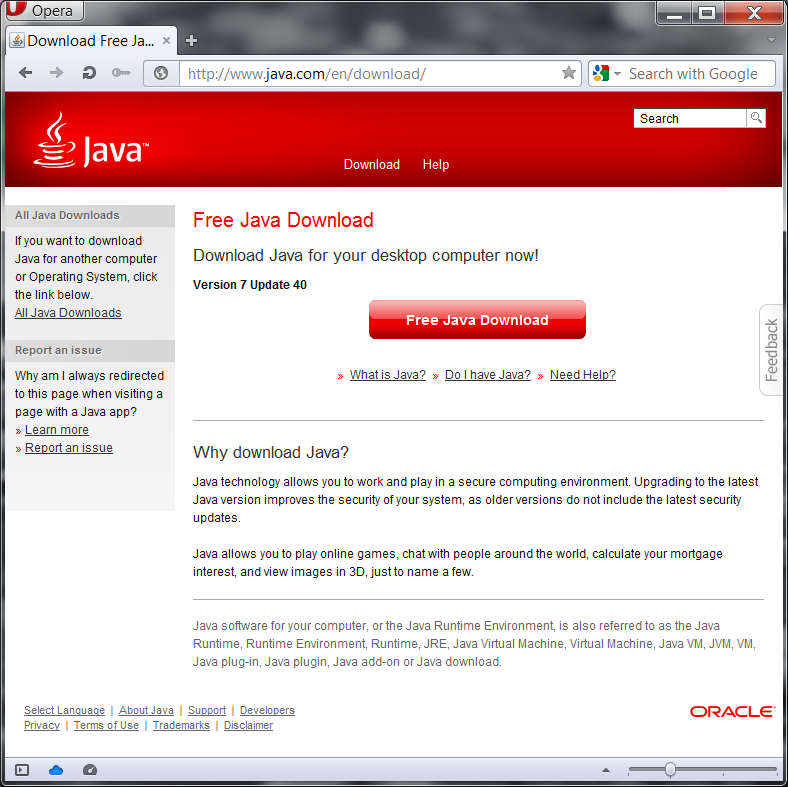
\includegraphics[scale=.4]{imgs/java-homepage-1.png}
%\end{center}

%\begin{center}
%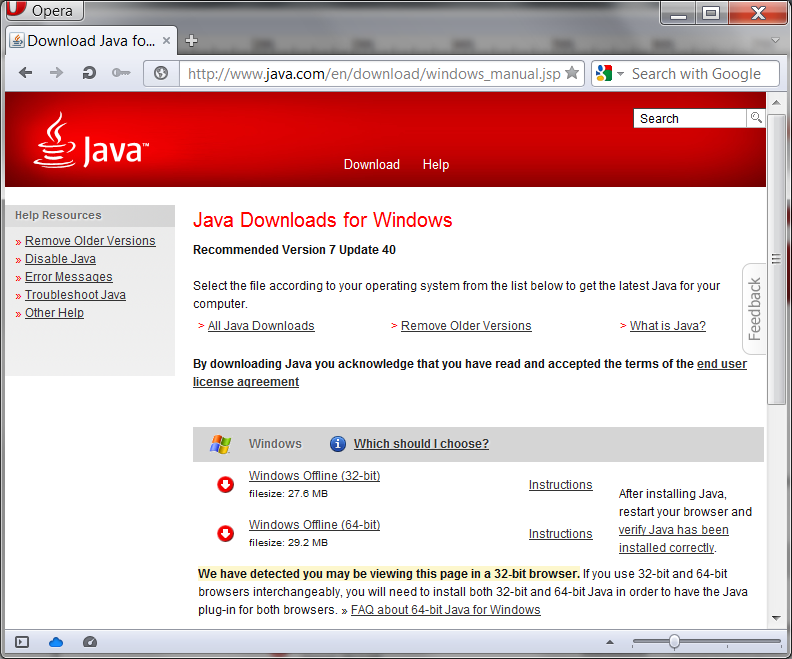
\includegraphics[scale=.4]{imgs/java-homepage-2.png}
%\end{center}

\subsection{Cygwin}

Das Cygwin Setup k�nnt ihr auf \url{http://cygwin.org/} herunterladen.

\begin{center}
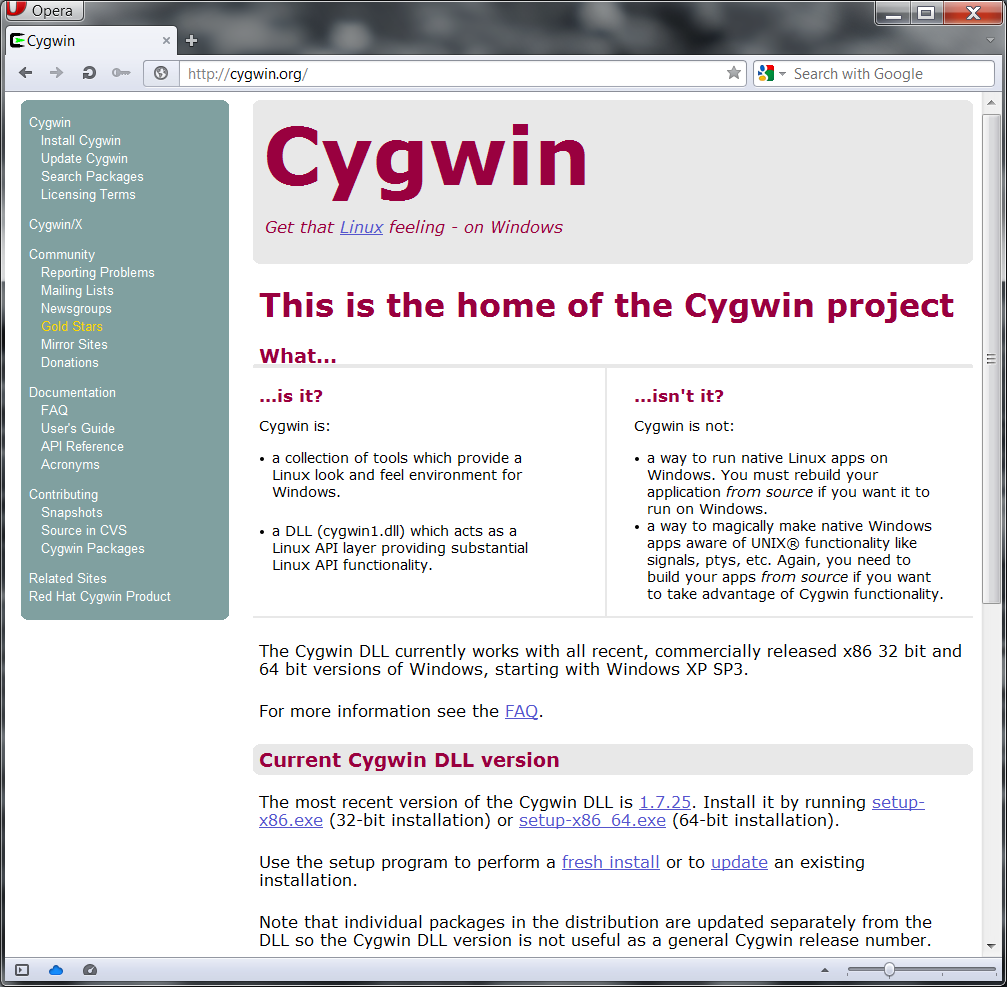
\includegraphics[scale=.4,width=.9\textwidth]{imgs/cygwin-homepage.png}
\end{center}

Es ist wichtig, Cygwin in einen Pfad ohne Leerzeichen o.�.\ zu installieren.
Belasst es also bitte bei dem empfohlenen Installationspfad
\texttt{C:\tbs{}cygwin} bzw.  \texttt{C:\tbs{}cygwin}.  W�hrend der
Installation w�hlt ihr bitte die folgenden Pakete aus:

\begin{itemize}
    \item gcc-core
    \item gdb
    \item make
\end{itemize}

\subsubsection{PATH setzen}

Danach m�sst ihr Cygwin zu der Umgebungsvariable PATH hinzuf�gen, damit eclipse
die ben�tigten Programme findet. Daf�r dr�ckt ihr \texttt{\winkey+R} und gebt
``\texttt{control sysdm.cpl,,3}'' (sic) ein. Es �ffnet sich ein Fenster
\textit{System Properties}.

\begin{center}
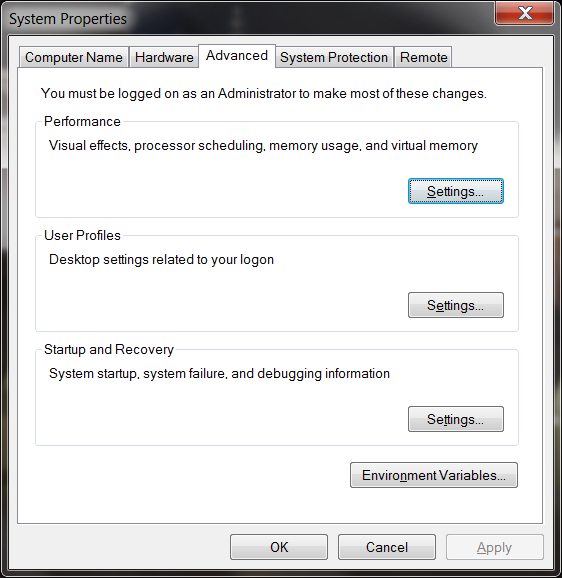
\includegraphics[scale=.4]{imgs/system_properties-advanced.png}
\end{center}

Dort klickt ihr auf \texttt{Environment Variables}.

\begin{center}
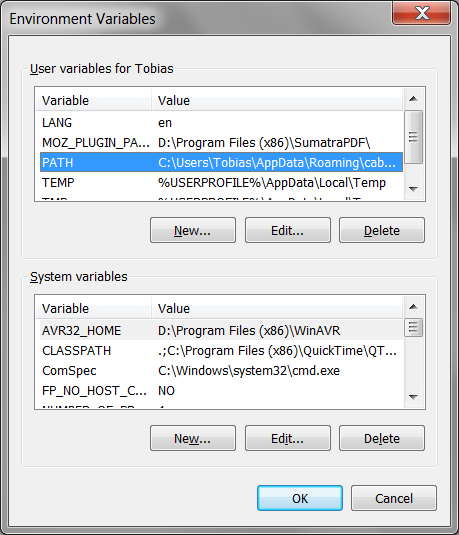
\includegraphics[scale=.4]{imgs/system_properties-advanced-env.png}
\end{center}

Schaut bitte oben unter \textit{User variables} nach, ob dort bereits eine
Variable mit dem Namen PATH existiert. Falls nicht, legt ihr eine neue Variable
mit dem Namen PATH und dem Wert ``\texttt{C:\tbs{}cygwin\tbs{}bin}'' an (falls
ihr Cygwin in \texttt{C:\tbs{}cygwin} installiert habt, sonst passt den Pfad
bitte entsprechend an). Falls die Variable bereits existiert, editiert ihr sie,
bewegt den Cursor ganz ans Ende des Textes (z.B.\ indem ihr auf eure
\texttt{Ende} Taste dr�ckt) und f�gt dort den gleichen Pfad ein, aber
\textit{mit einem Semikolon von dem existierenden getrennt}, also z.B.
``\texttt{;C:\tbs{}cygwin\tbs{}bin}''.

\begin{center}
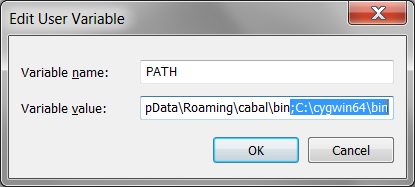
\includegraphics[scale=.4]{imgs/system_properties-advanced-env-set.png}
\end{center}


%\end{document}
}

\subsection{Bedienung von Cygwin}

Cygwin selbst l�sst sich nun vom Startmen� aus aufrufen und pr�sentiert sich als schwarzes Fenster mit einer blinkenden Eingabe, etwa wie folgt:

\begin{verbatim}
rattle@lucy ~
$
\end{verbatim}

Hinter dem Dollarzeichen erwartet Cygwin nun einen Befehl. Es gibt zahlreiche Befehle, einige wichtige haben wir hier f�r euch aufgelistet:

\begin{table}[H] \centering
\begin{tabular}{l|p{22em}} 
\bfseries{Befehl} & \bfseries{Effekt}  \\\hline
�ls� & Listet den Inhalt des derzeitigen Verzeichnisses auf.  \\
�mkdir <name>� & Erstellt einen Ordner mit dem angegebenen Namen \\
�cd <ordner>� & Wechselt in den angegebenen Ordner.   \\
�cp <quelle> <ziel>� & Kopiert die Datei quelle nach ziel. \\
�mv <quelle> <ziel>� & Verschiebt die Datei quelle nach ziel. \\
�rm <datei>� & L�scht eine Datei. \\
\end{tabular}
\label{table:cmd}
\caption{Befehle der Cygwin-Kommandozeile}
\end{table}

Ein einzelner Punkt steht f�r das derzeitige Verzeichnis und zwei Punkte f�r das dar�berliegende. Der Befehl �cd .� hat also keinen Effekt und �cd ..� bewegt sich einen Ordner nach oben.

Dar�ber hinaus ist jedes Programm, dass auf dem Computer (bzw. in Cygwin) installiert ist, ein Befehl. Durch eingabe von �notepad� beispielsweise �ffnet sich der Windows-Texteditor und der Befehl �gcc� ruft den Compiler auf. Nun wollen wir unser Hello World Programm aus \ref{helloworld} kompilieren und ausf�hren:

\begin{figure}[H]
\centering
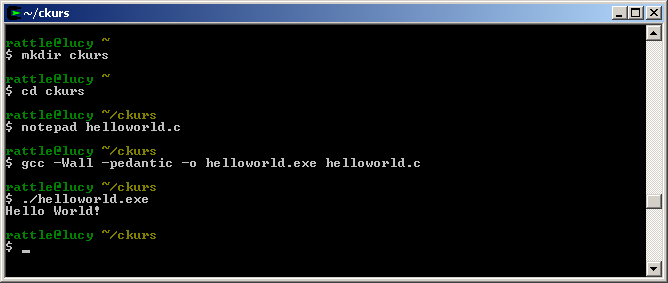
\includegraphics[width=11.9cm]{cygshell}
\caption{Kompilieren von ``Hello World'' unter Cygwin}
\end{figure}

Durch �notepad helloworld.c� erstellen wir die Textdatei �helloworld.c�. Es ist Konvention, dass Dateien, welche C-Quellcode enthalten, die Dateiendung �.c� erhalten. Wir bitten freundlich um Einhaltung dieser Konvention unter Androhung ritueller Enthauptung. Nach Tippen des oben angegebenen Quellcodes speichern wir die Datei und kehren zur Kommandozeile zur�ck. Der Befehl �gcc� hat folgendes Format:

\begin{alltt}
    gcc \opt{-Wall -pedantic} -o \ph{EXECUTABLE} \ph{QUELLDATEI}
\end{alltt}

wobei in diesem Fall unsere Quelldatei den Namen �helloworld.c� tr�gt. Als Name f�r die Executable bietet sich der Name �helloworld.exe� an, doch nat�rlich steht einem die Entscheidung hier frei. Die Option �-Wall� ist eine Abk�rzung f�r "`Warning: All"' und bedeutet, dass der Compiler alle Warnungen ausgibt. Warnungen sind unser wichtigstes Hilfsmittel, um sp�ter Fehler in Programmen zu finden und zu beheben.

Nachdem wir den gcc aufgerufen haben, wurde im gleichen Verzeichnis eine Datei erstellt, die �helloworld.exe� hei�t. Der Befehl �./helloworld.exe� besagt, dass die Datei �helloworld.exe� im derzeitigen Verzeichnis (der einzelne Punkt) ausgef�hrt werden soll. 


\section{Elementare Sprachkonstrukte}
\subsection{Kommentare}
Obgleich Programmiersprachen gedacht sind, um dem Menschen verst�ndlicher zu sein als der kryptische Maschinencode, k�nnen nur die wenigsten von uns C-Quellcode wie ein lustiges Taschenbuch lesen. Daher m�chte man h�ufig an verschiedenen Stellen im Quellcode sogenannte \df{Kommentare} einf�gen, d.h. Erl�uterungen und Erkl�rungen zum Programm, welche nicht vom Compiler als Befehle interpretiert werden sollen. Um einen Kommentar zu beginnen, verwendet man die Zeichenfolge �/*� und beendet ihn durch die Zeichenfolge �*/�. Ein Beispiel:

\begin{codes}[Hallo-Welt-Programm mit Kommentaren,label=hworld_with_comments]
/* HelloWorld v2.1a
   (c) 2008 by Jesko & Lars */
#include <stdio.h>
int main() {
  printf("Hello World\n");
  return 0; /* Programm fehlerfrei beendet */
} 
\end{codes}

\subsection{Variablen}
Ganz abstrakt ist ein Programm eine Maschinerie, die gewisse Daten erh�lt, und daraus neue Daten auf eine bestimmte Art und Weise berechnet. Daten treten in einem Programm stets in Form von sogenannten \df{Variablen} auf. Dabei ist eine Variable der Name f�r eine zusammenh�ngenden Region im Speicher des Computers, die durch ihren Datentyp eine Interpretation der dort gespeicherten Bits zugewiesen bekommt. Durch den Namen l�sst sich im C-Programm die Speicherregion auslesen oder neu beschreiben. Der Programmierer kann sich zu Beginn eines Programmblocks wie folgt Variablen deklarieren (erstellen):

\begin{alltt}
    \ph{DATENTYP} \ph{NAME}\opt{ = \ph{WERT}};
\end{alltt}

Wann immer wir Definitionen wie oben angeben, so bedeutet ein unterstrichenes Wort, dass an dieser Stelle verschiedenes stehen kann. F�r \ph{�NAME�} etwa wird der \df{Name} eingef�gt, welchen die Variable haben soll. Dies ist eine beliebige Zeichenfolge aus Buchstaben, Ziffern und Unterstrichen, welche nicht mit einer Ziffer beginnt. Der Name der Variablen sollte Aufschluss �ber ihren Zweck im Programm liefern. Variablennamen mit nur einem Buchstaben, obgleich in der Mathematik sehr verbreitet, sorgen bei Programmen in den meisten F�llen nur f�r Verwirrung. Ist ein Teil einer Definition grau gef�rbt, so ist dieser Teil optional. Wir bemerken, dass das Semikolon oben nicht mehr optional ist.

Tabelle \ref{table:datentypentabelle} gibt Aufschluss �ber die zur Verf�gung stehenden \df{Datentypen}, welche f�r \ph{�DATENTYP�} eingesetzt werden k�nnen. Ein �int� beansprucht stets weniger oder genauso viel Speicher wie ein �long int� und stets mehr oder genauso viel Speicher wie ein �short int�. Die gew�hnliche Gr��e in Bits, die ein �int� belegt, hat sich im Laufe der Jahrzehnte von $16$ �ber $32$ zu mittlerweile $64$ Bits gesteigert und k�nnte sich in der Zukunft weiter �ndern. 

Wir wollen noch etwas genauer verstehen, wie die verschiedenen ganzzahligen Datentypen zusammenh�ngen. Die Begriffe �signed� und �unsigned� sowie �short� und �long� sind bei der Deklaration einer �int�--Variablen optional. Wird einer der Ausdr�cke nicht angegeben, so wird ein vom Computer und vom Betriebsystem abh�ngiger Standard gew�hlt. Sollte allerdings einer dieser Begriffe angegeben werden, so kann �int� selbst weggelassen werden, etwa so:
\begin{codes}
    unsigned x;
\end{codes}

\begin{table} \centering
\begin{tabular}{|l|l|l|} \hline 
\bfseries{Variablentyp} & \bfseries{Deklaration} & \bfseries{Ausgabebefehl} \\\hline
Ganzzahl & �int v;� & �printf("%i\n", v);� \\\hline
Kleine Ganzzahl & �signed short int v;� & �printf("%hi\n", v);� \\\hline
Gro�e Ganzzahl & �signed long int v;� & �printf("%li\n", v);� \\\hline
Ganzzahl $\ge 0$ & �unsigned int v;� & �printf("%u\n", v);� \\\hline
Kleine Ganzzahl $\ge 0$ & �unsigned short int v;� & �printf("%hu\n", v);� \\\hline
Gro�e Ganzzahl $\ge 0$ & �unsigned long int v;� & �printf("%lu\n", v);� \\\hline
Byte (8 Bit) & �char c;� & �printf("%c\n", c);� \\\hline
Kleine Flie�kommazahl  & �float f;� & �printf("%f\n", f);� \\\hline
Gro�e Flie�kommazahl & �double d;� & �printf("%f\n", d);� \\\hline
\end{tabular}
\label{table:datentypentabelle}
\caption{Die Funktion printf wird sp�ter genau erl�utert werden}
\end{table}

Optional kann einer Variablen bereits bei der Deklaration ein \emph{Wert} zugewiesen werden. Diesen Vorgang bezeichnet man als \df{Initialisierung} der Variablen. Beispiel: 

\begin{codes}
    unsigned long pi = 3;  /* pi wird zu 3 initialisiert */
    unsigned long x;       /* x ist undefiniert */
    unsigned long y = pi;  /* y wird zu pi initialisiert */
\end{codes}

Achtung: Wird eine Variable nicht initialisiert, so ist sie \df{undefiniert}: Es ist unvorhersehbar, welchen Wert sie hat. Will man mehrere Variablen vom gleichen Typ deklarieren, so ist dies auch m�glich, indem man sie nach Angabe des Datentyps lediglich durch Kommata trennt. Damit ist
\begin{codes}
    unsigned long pi = 3, x, y = pi; 
\end{codes}
eine Kurzschreibweise f�r den Quellcode oben.

\subsection{Numerische Konstanten} \label{elementare_sprachkonstrukte:numerische_konstanten}
Ganzzahlige Konstanten sind uns bereits bei der Initialisierung von Variablen oben begegnet. Sie werden einfach als Folge von Ziffern in den Code eingegeben. Dabei k�nnen Zahlen zu unterschiedlichen Basen angegeben werden, nach folgender Regel:
\begin{enumerate}
\item Beginnt die Ziffernfolge \emph{nicht} mit der Ziffer �0�, so wird sie als ``gew�hnliche'' Zahlendarstellung im Dezimalsystem verstanden. 
\item Andernfalls, wenn die Ziffernfolge mit �0x� beginnt, so d�rfen au�er normalen Ziffern auch die Buchstaben �A� bis �F� in der Zahldarstellung verwendet werden. Diese wird dann als \df{Hexadezimalzahl} (Darstellung zur Basis $16$) interpretiert.
\item Andernfalls, wenn die Ziffernfolge mit �0� beginnt, wird sie als \df{Oktalzahl} (Darstellung zur Basis $8$) verstanden. In diesem Fall sind die Ziffern �8� und �9� nicht erlaubt.
\end{enumerate}
Dies ist insbesondere wichtig zu wissen, um Fehler zu vermeiden:
\begin{codes}
int x1 = 210; /*          x1 hat den Wert 210 */
int x2 = 070; /* Achtung: x2 hat den Wert 56  */
\end{codes}
Allerdings haben Konstanten auch einen Datentyp: Dieser Datentyp ist durch die Darstellung der Konstanten im Quellcode gegeben. Damit eine Konstante nicht als Ganzzahl, sondern als Flie�kommazahl interpretiert wird, so muss sie einen Punkt zwischen den Vorkomma- und Nachkommastellen enthalten. Zus�tzlich kann man wissenschaftliche Notation verwenden, was wir lediglich an einem Beispiel verdeutlichen wollen: 
\begin{codes}
  double pi = 3.141592653539793;  /* Kommadarstellung f�r ~Pi */
  double  c = 2.99792458e8;       /* wissenschaftliche Notation f�r ~Lichtgeschwindigkeit */ 
\end{codes}
Man kann Stellen vor und nach dem Punkt auch weglassen, diese werden dann automatisch zu $0$. Beispiel:
\begin{codes}
  double half = .5;
\end{codes}
\emph{Anmerkung}: Flie�kommazahlen k�nnen ausschlie�lich als Darstellung zur Basis $10$ angegeben werden. F�hrende Nullen werden bei der Angabe von Flie�kommakonstanten einfach ignoriert.

\subsection{Operatoren und Expressions} \label{sec:operatoren_und_expressions}
Eine \df{Expression} in C steht f�r einen Teil des Codes, welcher, ganz anschaulich ausgedr�ckt, einen Wert hat. Eine Variable ist beispielsweise bereits eine Expression, genau wie Konstanten.

Alle anderen Expressions in C entstehen aus Konstanten und Variablen durch deren Verkn�pfung mittels \df{Operatoren} und Klammerung. Abstrakt ausgedr�ckt ordnet ein Operator einem oder mehreren Werten einen neuen Wert zu. So sind etwa alle Grundrechenarten

\begin{table}[H] \centering
\begin{tabular}{|l|c|l|} \hline 
\bfseries{Operator} & \bfseries{Expression} & \bfseries{Wert der Expression} \\\hline
Addition & �a + b� & Summe von �a� und �b�  \\\hline
Subtraktion & �a - b� & Differenz von �a� und �b�  \\\hline
Multiplikation & �a * b� & Produkt von �a� und �b�  \\\hline
Division & �a / b� & Quotient von �a� und �b� \\\hline
Modulo & �a % b� & Rest einer Ganzzahldivision von �a� durch �b� \\\hline
\end{tabular}
\label{table:operatorentabelle:arithmetisch}
\caption{Arithmetische Operatoren}
\end{table}
sogenannte \df{bin�re} Operatoren (da sie zwei Werten einen Neuen zuweisen, n�mlich gerade das Rechenergebnis). Beispiele f�r Expressions sind �3+5*9� und �(pi+5)*9�. Dabei gilt wie gewohnt: ``Punkt- vor Strichrechnung''. Der Wert der Expression ist dann nat�rlich das Gesamtergebnis (beim ersten Beispiel also �48� und beim Zweiten �72�). Wir werden im Laufe des Kurses au�er den Grundrechenarten noch viele weitere Operatoren kennen lernen. Der Wert einer Expression kann durch den \df{Zuweisungsoperator} ``�=�'' \label{Op:Zuweisung} in einer Variablen gespeichert werden:

\begin{codes}
    pi = (pi+5)*9;  /* setzt die Variable pi auf (pi+5)*9 */
\end{codes}

Der Zuweisungsoperator entspricht also nicht dem mathematischen Gleichheitszeichen, sondern wird gelesen als ``wird gesetzt auf''. Wer sich nun fragt, warum dies ein Operator sein soll, sei gesagt, dass eine Zuweisung in C auch einen Wert hat, n�mlich gerade den Wert, der zugewiesen wird. Damit ist folgender Code korrekt:

\begin{codes}
    x = pi = x+5*9; /* entspricht x = (pi=x+5*9); */
\end{codes}

Hier wird also zun�chst der Wert von �(x+45)� in der Variablen �pi� gespeichert -- das Ergebnis dieser Zuweisungsoperation ist wiederum �(x+45)�, welches dann nach x geschrieben wird. Man sagt auch, der Zuweisungsoperator hat einen \df{Nebeneffekt}, da er nicht nur einen Wert zur�ckgibt, sondern in Folge seiner Auswertung auch den Inhalt einer Speicherzelle ver�ndert.  
Da jede Expression einen Wert hat, hat sie auch einen Datentyp. Gelegentlich m�chte man durch Operatoren auch Expressions verkn�pfen, die formal unterschiedliche Datentypen haben -- in diesem Fall muss eine der Expressions in eine Expression vom anderen Typ konvertiert werden. Diesen Vorgang nennt man \df{typecasting}. In vielen F�llen, wie etwa der Verkn�pfung zweier Expressions mit Ganzzahltypen, nimmt C diese Konvertierung automatisch und meistens auch so vor, wie man es sich w�nscht. M�chte man dennoch manuell eine Typkonvertierung durchf�hren, so geschieht dies durch folgende Syntax: \label{Op:Typecast}
\begin{alltt}
    (\ph{DATENTYP}) (\ph{EXPRESSION})
\end{alltt}
Als Beispiel k�nne man etwa eine Flie�kommazahlen in eine Ganzzahl konvertieren, indem man schreibt:
\begin{codes}
	double pi = 3.14159;
	unsigned n = (unsigned) pi;
\end{codes}
Die Konvertierung von Flie�kommazahlen in Ganzzahlen geschieht durch Runden in Richtung $0$. All dies wirft ein neues Licht auf die oben vorgestellten Rechenoperationen: Diese haben n�mlich, abh�ngig vom Typ ihrer Argumente, eine unterschiedliche Arbeitsweise.



\begin{itemize}
\item Dividieren wir zwei Ganzzahlen, so wird eine Ganzzahldivision durchgef�hrt und der dabei entstehende Rest verworfen; also ergibt �1/2� den Wert �0� und �7/3� h�tte den Wert �2�. Durch explizites Typecasting l�sst sich hier ein anderes Verhalten erzwingen schaffen:
\begin{codes}
    unsigned x = 1, y = 2;
    double half = (double)x/y; /* nun hat half den Wert 0.5 */
\end{codes}
\item Dividiert man eine Ganzzahl durch eine Flie�kommazahl oder umgekehrt, so wird die Ganzzahl konvertiert und man erh�lt das (mehr oder minder) korrekte Ergebnis der Rechnung als Flie�kommazahl.
\item Generell gilt: Verkn�pfen wir eine Flie�kommazahl mit einer Ganzzahl, so wird diese in eine Flie�kommazahl konvertiert, und das Ergebnis ist ebenfalls eine Flie�kommazahl.
\end{itemize}

Es gibt nun noch einen weiteren n�tzlichen Rechenoperator, der bei einer Ganzzahldivision das Ergebnis verwirft und statt dessen den Rest als Ergebnis liefert: Der sogenannte \df{Modulo}-Operator, �%� (ein Prozentzeichen). So w�re etwa �(6%5)� eine Expression mit dem Wert �1�. Dieser Operator funktioniert nur mit Ganzzahlen.

H�ufig hat man in der Programmierung Zuweisungen der Form �a = a �$\times$� b�, wobei $\times$ einer der bisherigen, bin�ren Rechenoperatoren ist. Daf�r gibt es die Kurzschreibweise �a �$\times$�= b� \label{Op:Kurz}. Ein Beispiel: �a += 1� w�rde den Wert von �a� um �1� erh�hen. Die Situation, eine Variable um  zu de- oder inkrementieren, ergibt sich sehr h�ufig. Daf�r verwendet man folgenden un�ren Operatoren \label{Op:IncDec}.

\begin{table} [H] \centering
\label{table:kurzschreibweisen}
\begin{tabular}{|c|c|l|c|} \hline 
\bfseries{Operator} & \bfseries{Art} & \bfseries{Wirkung} & \bfseries{Wert der Expression} \\\hline
�a++� & postfix & inkrementiere �a� & �a� \\\hline
�++a� & pr�fix & inkrementiere �a� & �a+1� \\\hline
�a--� & postfix & dekrementiere �a� & �a� \\\hline
�--a� & pr�fix & dekrementiere �a� & �a-1� \\\hline
	\end{tabular}
\caption{Kurzschreibweisen}
\end{table}

\emph{Anmerkung:} Es gibt Expressions, welche aufgrund ihrer Nebeneffekte nicht eindeutig sind, etwa �i=i+++i�. Diese Expression ist syntaktisch korrekt, doch es gibt keinen offiziellen Standard f�r ihren Wert. Man bezeichnet solche Expressions als \df{undefiniert}. Jeder Compiler hat bei derartigen Situationen das Recht, �ber die weitere Verfahrensweise zu entscheiden (Er k�nnte etwa die Expression auf eine m�gliche Art und Weise auswerten oder einen Fehler erzeugen). Man sollte solche Expressions tunlichst vermeiden.



\subsection{Formalit�ten: Statements und Expressions}
C-Programme setzen sich aus einer oder mehreren \df{Statements} zusammen. Wir haben bereits ein Statement kennen gelernt: Die Variablendeklaration. Au�erdem kann man eine Expression zu einem Statement machen, indem man sie durch ein Semikolon abschlie�t. Ein Beispiel daf�r ist die Zuweisung, die wir bereits in \ref{sec:operatoren_und_expressions} kennen gelernt haben. Dar�ber hinaus kann man auch eine \df{Expressionliste} als Statement auswerten lassen: Dies ist eine durch Kommata separierte Liste von Expressions, welche durch ein abschlie�endes Semikolon zu einem Statement f�hrt, in dem die Expressions der Reihe nach ausgewertet werden:

\begin{alltt}
    \ph{EXPRESSION 1}, \ph{EXPRESSION 2}, \ldots, \ph{EXPRESSION n};
\end{alltt}
Dies scheint zun�chst nicht besonders n�tzlich zu sein, da wir die einzelnen Expressions durch Semikolons auch einzeln zu Statements machen k�nnen -- im Zusammenspiel mit anderen Statements jedoch kann es sich als n�tzlich erweisen, mehrere Expressions als ein { \itshape einzelnes} Statement zusammenfassen zu k�nnen. In Wahrheit ist eine Expressionliste ebenfalls eine Expression: Das Komma ist ein bin�rer Operator \label{Op:Komma}, welcher seine beiden Argumente auswertet und den zweiten als Ergebnis liefert: Wert und Typ einer Expressionliste sind also immer Wert und Typ der letzten Expression in der Liste.

Ein weiteres, bereits bekanntes Statement ist der \df{Block}, welcher einfach mehrere Statements zu einem Statement zusammenfasst:

\begin{alltt}
    \{ \ph{STATEMENT 1} \ph{STATEMENT 2} \ldots \ph{STATEMENT n} \}
\end{alltt}

Wichtig: Variablendeklarationen sind Statements, die nicht an jeder Stelle des Quellcodes verwendet werden d�rfen. Variablendeklarationen m�ssen immer \emph{die ersten Statements eines Blocks sein}. Die Variablen, die zu Beginn eines Blocks deklariert werden, geh�ren in gewisser Weise zu diesem Block. Nachdem der Block endet, werden die Variablen verworfen. Dar�ber hinaus kann eine Variablendeklarion in einem Block eine Variable des ihn umschlie�enden Blocks {\itshape �berdecken}: Das hei�t, in einem Block k�nnen Variablen deklariert werden, die au�erhalb des Blocks bereits existieren. Diese beiden Variablen repr�sentieren in diesem Fall \emph{zwei unterschiedliche Speicherbereiche}, und innerhalb des Blocks k�nnen wir nur noch diejenige Variable verwenden, welche auch im Block deklariert wurde. Ein Beispiel:


\begin{codes}[Beispiel f�r �berdeckung,label=code:ueberdeckung]
#include <stdio.h>
int main() {             /* Hier beginnt Block 1 */
    int i = 4;
    int j = 6;
    {                      /* Hier beginnt Block 2 */
        int i=3;
        printf("%i\n",i);  /* Gibt 3 aus */
        printf("%i\n",j);  /* Gibt 6 aus */
    }                      /* Hier endet Block 2 */
    printf("%i\n",i);      /* Gibt 4 aus */
}                          /* Hier endet Block 1 */
\end{codes}

\subsection{If-Else-Statement}
Einfache Rechenoperatoren erlauben uns nicht, komplexe Algorithmen zu implementieren -- es fehlt die M�glichkeit, abh�ngig vom  {\itshape Ergebnis} einer Operation {\itshape unterschiedlichen} Code auszuf�hren. Um dies zu erm�glichen, lernen wir nun das erste Programmierstatement kennen: Das If-Else-Konstrukt:

\begin{alltt}
    if ( \ph{BEDINGUNG} ) \ph{BEFEHL 1}
    \opt{else \ph{BEFEHL 2}}
\end{alltt}

wobei die Bedingung eine beliebige Expression und die Befehle jeweils ein beliebiges Statement (meistens ein Block) sein k�nnen. Es wird der erste Befehl ausgef�hrt, sofern die Bedingung einen Wert ungleich $0$ hat. Ansonsten, falls durch �else� angegeben, der zweite.

\subsection{Logische- und Vergleichsoperatoren}
\label{sec:logischeundvergleichsoperatoren}
F�r die Bedingung im If-Else-Statement lernen wir noch einige weitere Operatoren kennen, die sogenannten \df{Vergleichsoperatoren}:

\begin{table} [H] \centering
\label{table:vergleichsoperatoren}
\begin{tabular}{|l|c|} \hline 
\bfseries{Operator} & \bfseries{Syntax} \\\hline
Pr�fen auf Gleichheit&�a == b� \\\hline
Pr�fen auf Ungleichheit&�a != b� \\\hline
Pr�fen, ob �a� echt gr��er als �b� ist&�a > b� \\\hline
Pr�fen, ob �a� echt kleiner als �b� ist&�a < b� \\\hline
Pr�fen, ob �a� gr��er oder gleich �b� ist&�a >= b� \\\hline
Pr�fen, ob �a� kleiner oder gleich �b� ist&�a <= b� \\\hline
\end{tabular}
\caption{Vergleichoperatoren}
\end{table}

Diese Operatoren liefern immer die Werte �1� oder �0�, abh�ngig vom Ergebnis des Vergleiches. Damit wird das If-Else-Statement bereits zu einem m�chtigen Werkzeug. Als Beispiel ein Codesegment, dass die Signumsfunktion f�r einen Eingabewert �x�  implementiert:

\begin{codes}[Signumsfunktion,label=code:signuminline]
if (x < 0)      /* falls x kleiner als 0 ist: */
  y = -1;       /* das Signum ist -1 */
else            /* Ansonsten (falls x gr��ergleich 0): */
  y = (x != 0); /* falls x Null, wird y Null, sonst 1 */
\end{codes}

Um Vergleiche logisch zu verkn�pfen, gibt es dar�ber hinaus auch noch die sogenannten \df{logischen Operatoren} (\ref{table:logischeoperatoren}). Dies sind ebenfalls bin�re Operatoren (bis auf das logische Nicht), welche zwei Expressions die Werte �0� oder �1� zuweisen. 

\begin{table} [H]  \centering
\label{table:logischeoperatoren}
\begin{tabular}{|l|c|} \hline 
\bfseries{Operator} & \bfseries{Syntax} \\\hline
Logisches Und & �A && B� \\\hline
Logisches Oder & �A || B� \\\hline
Logische Verneinung & �!A� \\\hline
\end{tabular}
\caption{Logische Operatoren}
\end{table} 

Die Ergebnisse der Logischen Operatoren lassen sich am einfachsten durch Wertetabellen veranschaulichen. Siehe dazu \ref{table:logischeoperatorenwerte}.

\begin{table} [H]  \centering
\label{table:logischeoperatorenwerte}
\begin{tabular}{|r|r|c|c|c|} \hline 
\bfseries{�A�} & \bfseries{�B�} & \bfseries{�A && B�} & \bfseries{�A || B�} & \bfseries{�!A�} \\\hline
$0$ & $0$ & $0$ & $0$ & $1$ \\\hline
$0$ & $\neq 0$ & $0$ & $1$ & $1$ \\\hline
$\neq 0$ & $0$ & $0$ & $1$ & $0$ \\\hline
$\neq 0$ & $\neq 0$ & $1$ & $1$ & $0$ \\\hline
\end{tabular}
\caption{Logische Operatoren}
\end{table}

Es gibt jedoch noch eine wichtige Eigenart dieser Operatoren zu erw�hnen: Die logischen Operatoren werten nur so viele ihrer Argumente aus, bis das Ergebnis der Verkn�pfung bereits feststeht. So w�rde etwa bei der Auswertung von �(1 || x--)� die Variable �x� {\itshape nicht} dekrementiert, da das Ergebnis der Operation bereits bei der Auswertung von �1� feststeht. Dies ist selbstverst�ndlich nur von Bedeutung, sofern eine der auszuwertenden Expressions einen Nebeneffekt hat.

\subsection{Der Schleifen erster Teil: while}
Wollen wir einen bestimmten Codeblock mehrfach ausf�hren, so verwenden wir ein Statement, was als \df{Schleife} bezeichnet wird. Eine Schleife wiederholt die Befehle so lange, wie eine bestimmte Expression ungleich �0� ist. Die Syntax

\begin{alltt}
    while (\ph{BEDINGUNG}) \ph{BEFEHL}
\end{alltt}

weist den Computer an, zu pr�fen, ob die Expression \ph{�BEDINGUNG�} ungleich �0� ist. Ist dies der Fall, so wird das Statement \ph{�BEFEHL�} ausgef�hrt und wir fangen wieder von vorne mit dem Pr�fen der Bedingung an. Andernfalls wird die Schleife beendet. Meistens sollten die Befehle daf�r sorgen, dass \ph{�BEDINGUNG�} irgendwann zu �0� auswertet, indem etwa Variablen ver�ndert werden. Man kann jedoch ebensogut eine Endlosschleife programmieren:

\begin{codes}[Endlosschleife,label=code:endlosschleife]
while(1); /* leeres statement: tue nichts, und das f�r immer */
\end{codes}

Wir wollen ein Beispiel angeben, welches die Geometrische Reihe $\sum_{n=0}^\infty q^n = \frac{1}{1-q}$ ausrechnet:

\begin{codes}[Geometrische Reihe,label=code:geometrischereihe]
double q = 0.2;
double x = 1.0, y = 0.0;  /* Hilfsvariablen */
while (x > 1e-10) {       /* Solange x nicht zu klein ist */
  y = y+x;                /* y speichert die Partialsummen */
  x = x*q;                /* Berechne den n�chsten Summanden */
}
/* Ergebnis steht jetzt in y */
\end{codes}

Dieses Beispiel zeigt anschaulich, dass Programme deutlich aufw�ndiger sein k�nnen, als sie m�ssen. Wir h�tten ebenso gut �y=1./(1.-q);� schreiben k�nnen, was der Computer in einem Bruchteil der Zeit berechnen k�nnte. Man sollte sich immer bem�hen, nicht unn�tig Rechenzeit zu vergeuden. 
 
Wenn man das Statement \ph{�BEFEHL�} gerne Ausf�hren m�chte, bevor das erste Mal gepr�ft wird, ob \ph{�BEDINGUNG�} zu �0� auswertet, so kann man eine do-while-Schleife verwenden:

\begin{alltt}
    do \ph{BEFEHL} while(\ph{BEDINGUNG});
\end{alltt}

Man bemerke hier das zwingend erforderliche Semikolon am Ende.


\subsection{Der Schleifen zweiter Teil: for}
Die while-Schleife l�sst sich verallgemeinern zur �for�-Schleife, dem folgenden Konstrukt:

\begin{alltt}
    for( \ph{\opt{INITIALISIERUNG}}; \ph{\opt{BEDINGUNG}}; \ph{\opt{STEP}} )
      \ph{BEFEHL}
\end{alltt}

wobei wir dies wie folgt durch eine while-Schleife modellieren k�nnten, sofern die Bedingung angegeben ist:

\begin{alltt}
    \ph{INITALISIERUNG};
    while ( \ph{BEDINGUNG} ) \{
      \ph{BEFEHL}
      \ph{STEP};
    \}
\end{alltt}

Damit sind also die Initialisierung, der Step und die Bedingung jeweils eine Expression. Der Befehl ist, wie immer, ein einzelnes Statement (meistens ein Code-Block). Das Beispiel aus dem letzten Abschnitt kann man also so umschreiben:

\begin{codes}[Geometrische Reihe mit einer For-Schleife,label=code:geometrischreihefor]
double x,y,q = 0.2; 
for (x=1.,y=0.; x>1e-10; x = x*q)
 y = y+x;
\end{codes}

L�sst man bei der �for�-Schleife die Bedingung weg, bricht die Schleife nicht ab. Genauer: Die Schleife verh�lt sich so, als w�re die Bedingung die konstante Expression �1�. Step oder Initialisierung sind ebenfalls optional und k�nnen weggelassen werden -- also ist folgende Schleife eine Endlosschleife: �for(;;);�

Es gibt zwei besondere Statements, welche innerhalb von Schleifen verwendet werden k�nnen:

\begin{table} [H] 
\label{table:schleifenbefehle} \centering
\begin{tabularx}{\textwidth}{|l|X|} \hline 
\bfseries{Statement} & \bfseries{Effekt} \\\hline
�break;� & Schleife abbrechen bzw. zum n�chsten Statement nach der Schleife springen. In einer �for�-Schleife wird der Step noch einmal ausgef�hrt. \\\hline
�continue;� & Nur diesen Schleifendurchlauf abbrechen (zum Step springen). \\\hline
\end{tabularx}
\caption{Spezielle Schleifenbefehle}
\end{table}

Bei einer �for�-Schleife sorgt ein �continue�-Statement also daf�r, dass der Step noch ausgef�hrt wird, bevor die Bedingung abgefragt wird und dann evtl. der n�chste Schleifendurchlauf beginnt.

\section{Funktionen}
Funktionen sind ein grundlegendes und wichtiges Konzept der Programmierung. Sie erm�glichen es, h�ufig ben�tigte Programmzeilen als ``Unterprogramm'' zusammenzufassen. An anderen Stellen im gleichen Programm kann man dann durch einen sogenannten \df{Aufruf} der Funktion dorthin verzweigen. In der Funktion selbst kann man durch das �return� - Statement daf�r sorgen, dass die Ausf�hrung an der Stelle fortgesetzt wird, an der die Funktion aufgerufen wurde.
Wie ihre mathematischen �quivalente k�nnen Funktionen Argumente erhalten und einen R�ckgabewert besitzen. 

\subsection{Funktionsdefinitionen}
Eine \df{Funktionsdefinition} hat folgende Form:

\begin{alltt}
    \ph{R�CKGABETYP} \ph{FUNKTIONSNAME}(
        \ph{PARAMETERTYP 1} \ph{PARAMETERNAME 1},
        \ph{PARAMETERTYP 2} \ph{PARAMETERNAME 2}, 
        \ldots,
        \ph{PARAMETERTYP n} \ph{PARAMETERNAME n} ) \{
      \ph{BEFEHLE}
    \}
\end{alltt}
Der R�ckgabetyp ist hierbei ein beliebiger Datentyp - dieser bestimmt, welchen Datentyp der Ausdruck des Funktionsaufrufes hat. Ein \df{Funktionsaufruf} \label{Op:Funktionsaufruf} hat die Syntax:

\begin{alltt}
    \ph{FUNKTIONSNAME} ( \ph{PARAMETER 1}, \ldots, \ph{PARAMETER n} )
\end{alltt}

Dies bedeutet, dass eine Funktion ein vom Programmierer neu definierter Operator ist: Sie weist einem oder mehreren Werten einen neuen Wert (den R�ckgabewert) zu. 

Bei jedem Funktionsaufruf werden zun�chst neue Variablen \ph{�PARAMETERNAME 1�} bis \ph{�PARAMETERNAME n�} erstellt, welche vom in der Funktionsdefinition angegebenen Datentyp sind. Dann werden die Expressions \ph{�PARAMETER 1�} bis \ph{�PARAMETER n�} ausgewertet und den Variablen in der entsprechenden Reihenfolge zugewiesen. Anschlie�end werden die Befehle in der Funktionsdefinition ausgef�hrt, bis der Wert berechnet wurde, den der Funktionsaufruf haben soll. Durch das folgende Statement beendet die Funktion sich selbst augenblicklich und legt ihren sogenannten \df{R�ckgabewert} fest: Der Wert des Funktionsaufrufes.

\begin{alltt}
    return \ph{R�CKGABEWERT};
\end{alltt}

Die Parameter in der Funktionsdefinition sind Variablendeklarationen, deren Initialisierung durch den Funktionsaufruf statt findet. Sie geh�ren zum Block der Funktionsdefinition und k�nnen (sollten) dort zur Berechnung des R�ckgabewerts verwendet werden -- Dennoch kann eine Funktion selbstverst�ndlich zu Beginn weitere, interne Variablen erstellen.

Innerhalb der Funktion sind dies aber insgesamt die \emph{einzigen} Variablen, auf die direkt (mit Namen) zugegriffen werden kann. Wir wollen nun Code f�r eine Funktionsdefinition vorstellen, welche das Signum einer Ganzzahl ausrechnet (siehe auch \ref{sec:logischeundvergleichsoperatoren}) und diese Funktion dann aufrufen:

\begin{codes}[Funktionsdefinition und -aufruf,label=code:funktionsbeispiel]
#include <stdio.h>

int sign( int x ) {
  if (x < 0) return -1;
  else return (x != 0);
}

int main() {
  printf("%i\n", sign(-5));  /* Wird -1 ausgeben. */
  return 0;
}
\end{codes}

Noch ein Beispiel: 

\begin{codes}[Funktion zum Berchnen ganzer Potenzen von Flie�kommazahlen]
#include <stdio.h>

/* berechnet zahl hoch exponent */
double potenz(double zahl, unsigned int exponent) { 
  double ergebnis;
  for (ergebnis = 1.0; exponent; exponent--) 
    ergebnis *= zahl;
  return ergebnis;
}

int main() {
  printf("%f\n", potenz(0.5, 4) );  /* Wird 0.0625 ausgeben. */
  return 0;
}
\end{codes}

Wir k�nnen nun zum ersten mal feststellen, welche genaue Form ausf�hrbarer C-Quellcode hat: Dieser setzt sich n�mlich aus Funktionsdefinitionen zusammen, welche wiederum aus Statements bestehen, die bei Aufruf der Funktion in angegebener Reihenfolge ausgef�hrt werden. Es muss eine Funktion mit dem Namen �main� geben, welche zu Beginn des Programms gestartet wird.

\label{bisschenvoid} Wir lernen an dieser Stelle noch einen neuen Datentyp kennen, den Datentyp �void�. Man kann keine �void�-Variablen deklarieren, denn eine Expression mit Datentyp �void� hat \emph{keinen} Wert. Allerdings gibt es Funktionen mit \emph{R�ckgabetyp} �void�, welche man auch als Prozeduren bezeichnet. Eine Prozedur muss kein return-Statement enthalten, kann jedoch das leere return-Statement �return;� verwenden, um sich selbst zu beenden. 

\begin{codes}[Beispiel f�r eine Prozedur,label=code:prozedurbeispiel]
#include <stdio.h>

void printInt(int x) { 
  printf("%i\n",x); 
}

int main() {
  printInt(42); /* gebe 42 auf der Kommandozeile aus */
  return 0;
}
\end{codes}

\subsection{Funktionsdeklaration vs. Funktionsdefinition}

M�chte man eine Funktion aufrufen, so muss die Definition dieser Funktion im Quellcode vor dem Funktionsaufruf liegen, da der Compiler die aufzurufende Funktion bereits ``kennen'' muss, damit er einen Aufruf korrekt in Maschinencode �bersetzen kann: Dazu muss er wenigstens wissen, wie genau die Funktionsargumente und der R�ckgabetyp aussehen. Man kann diese Informationen jedoch angeben, bevor man die Funktion tats�chlich definiert, indem man lediglich eine \df{Funktionsdeklaration} verwendet. Dieses Statement sieht wie folgt aus:

\begin{alltt}
    \ph{R�CKGABETYP} \ph{FUNKTIONSNAME}(
        \ph{PARAMETERTYP 1} \ph{\opt{PARAMETERNAME 1}},
        \ldots,
        \ph{PARAMETERTYP n} \ph{\opt{PARAMETERNAME n}} );
\end{alltt}

Die Deklaration enth�lt also nur den sogenannten \df{Funktionskopf}, in dem alle f�r den Compiler wichtigen Informationen enthalten sind. Nachdem die Funktion deklariert ist, kann man sie im nachfolgenden Quellcode verwenden. An irgendeiner Stelle muss allerdings dann die tats�chliche Definition stehen. Hier ein Beispiel, welches ohne dieses Sprachkonstrukt gar nicht m�glich w�re:

\newpage
\begin{codes}[Funktionsdeklarationen sind notwendig,label=code:funktionsdeklaration]
#include <stdio.h>

/* Funktionsdeklarationen */
int ungerade(int);  /* diese Deklaration ist notwendig. */
int   gerade(int);  /* diese Deklaration nicht, ist aber huebsch. */

/* Funktionsdefinitionen */
int gerade(int n) {
/* testet, ob n gerade ist */
  if (n == 0) return 1;
  else return ungerade(n-1); /* wir m�ssen "ungerade" kennen */
}
int ungerade(int n) { /* testet, ob n ungerade ist */
  if (n == 0) return 0;
  else return gerade(n-1);
}

int main() {
  if ( gerade(5) ) {
    printf("Verkehrte Welt\n");
    return 1;
  } else return 0;
}
\end{codes}

Die Umsetzung dieser Funktionen ist nat�rlich haarstr�ubend ineffizient, umst�ndlich und unverst�ndlich. Wir konnten jedoch kein Besseres Beispiel f�r Funktionen finden, die sich auf diese Art und weise gegenseitig aufrufen: Man bezeichnet dies auch als \df{indirekte Rekursion}.

\subsection{Modulares Programmieren und Linken}
Die Kompilierung von gro�en Programmen zu schnellem und effizientem Maschinencode bedarf eines deutlich merkbaren Rechenaufwands. W�hrend der Weiterentwicklung oder Fehleranalyse solcher Programme m�ssen allerdings st�ndig Teile des Programmcodes ver�ndert werden und es w�re zu zeitaufw�ndig, das gesamte Programm st�ndig neu zu kompilieren - insbesondere, da sich ja nur gewisse Teilbereiche des Programms �ndern - etwa nur eine bestimmte Funktion. Man geht deswegen dazu �ber, einzelne Teile eines Programms so voneinander zu trennen, dass der Compiler sie unabh�ngig voneinander in Maschinencode �bersetzen kann. Diese Teile nennt man auch \df{Module}.

Nachdem ein solches Modul kompiliert wurde, ist es nat�rlich kein lauff�higes Programm - insbesondere verwendet das Modul unter Umst�nden Funktionen, deren Programmcode sich in anderen Modulen befindet. Um diese Abh�ngigkeiten aufzul�sen, wird in der Schlussphase der Codegenerierung ein Programm (der \df{Linker}) gestartet, um die kompilierten Module zu einem lauff�higen Programm zusammenzuf�gen. Diesen Vorgang bezeichnet man dementsprechend als \df{Linken}. Ein Modul in C ist zun�chst eine Datei mit Dateiendung ``c''. Jede solche �.c�-Datei wird von dem Compiler zu einer sogenannten \df{Objektdatei} kompiliert, welche das kompilierte Modul darstellt. Diese Objektdatei enth�lt Informationen dar�ber, welche Funktionen das Modul enth�lt und welche Funktionen von dem Modul aus anderen Modulen ben�tigt werden. Sind einmal alle Objektdateien erstellt, l�st der Linker die Abh�ngigkeiten zwischen ihnen auf und f�gt die Objektdateien zu einem lauff�higen Programmcode zusammen. Dieser Vorgang ist unabh�ngig von der Kompilierung.

Bei der Kompilierung ist es jedoch erforderlich, dass Funktionen definiert werden, bevor sie im Quellcode danach verwendet werden. Existiert etwa eine Quellcodedatei �moremath.c�, welche unter anderem eine Funktion
\begin{codes}
    unsigned fibonacci(unsigned n)
\end{codes}
beinhaltet, so k�nnte man die folgende �main.c� nat�rlich trotzdem nicht erfolgreich kompilieren, da zumindest eine Deklaration der Funktion fehlt:

\begin{codes}[Fehlende Deklaration,label=code:fehlendedeklaration]
#include <stdio.h>
/* Hier fehlt eine Deklaration oder �hnliches */
int main() {
  unsigned j;
  for (j=1; j<10; j++) 
    printf("%u\n", fibonacci(j));
  return 0;
}
\end{codes}

Man mache sich klar, dass dies ein Problem des Compilers und v�llig unabh�ngig vom Linker ist.  Um dieses Problem zu l�sen, geh�rt zu jedem Modul auch eine \df{Headerdatei} mit der Dateiendung ``h'', welche den gleichen Namen wie die Quellcodedatei des Moduls erh�lt. Diese enth�lt nur   Funktionsdeklarationen. Im Sinne des obigen Beispiels s�he die Headerdatei �moremath.h� etwa so aus:

\begin{codes}[Header-Datei f�r das moremath-Modul,label=code:moremathheader]
unsigned faculty(unsigned n);   /* berechnet n! */
unsigned fibonacci(unsigned n); /* berechnet die n-te Fibonaccizahl */
\end{codes}

Also enth�lt die Headerdatei lediglich Informationen �ber die Verwendung der Funktionen, die sich im zugeh�rigen Modul befinden, damit eine Kompilierung mit voneinander getrenntem Code �berhaupt erst m�glich wird. Mit dieser Datei ist �main.c� in folgender Variante nun kompilierbar:

\newpage
\begin{codes}[Deklaration fehlt nun nicht mehr,label=code:mitdeklaration]
#include <stdio.h>
#include "moremath.h"
int main() {
  unsigned j;
  for (j=1; j<10; j++)
    printf("%u\n", fibonacci(j));
  return 0;
}
\end{codes}

Die Headerdateien von selbstgeschriebenen Modulen werden durch die �#include� - Anweisung direkt in den Quellcode eingef�gt (kopiert) . Die Headerdateien eigener Module werden mit Anf�hrungszeichen angegeben, Headerdateien von Systemmodulen mit spitzen Klammern. In der Tat gibt es bereits im System vorhandene Modul wie etwa �stdio� und �math�, welche sich in ihrer Funktionsweise nicht von selbst erstellten Modulen unterscheiden. Das Modul �moremath.c� k�nnte nun wie folgt aussehen:

\begin{codes}[Das moremath-Modul,label=code:moremathmodul]
#include "moremath.h"

unsigned faculty(unsigned n) {
  unsigned f = 1;
  for (;n;n--) f *= n;
  return f;
}

unsigned fibonacci(unsigned n) {
  if (n < 2) return 1;
  else return fibonacci(n-1) + fibonacci(n-2);
}
\end{codes}

Die Quellcodedatei bindet f�r Gew�hnlich ihre zugeh�rige Headerdatei ein. Dies hat viele Vorteile, die in Zukunft noch klarer werden, doch einen Grund kenne wir bereits: Sollten die Funktionen eines Moduls sich gegenseitig verwenden, so vermeiden wir durch Einf�gen aller Deklarationen zu Anfang Compilerfehler.

Zusammenfassung: Der Compiler ist w�hrend der Kompilierung lediglich auf vollst�ndige Deklarationen aller verwendeten Funktionen angewiesen. Diese befinden sich in den jeweiligen Headerdateien. Ist die Kompilierung abgeschlossen, muss der Linker aus einer Menge von kompilierten Modulen ein Programm erstellen. Dazu sucht er zun�chst das Modul, welches die �main� Funktion enth�lt, da an dieser Stelle die Ausf�hrung des Programms beginnen soll. Von diesem Modul ausgehend sucht der Linker nun zu jedem noch nicht verkn�pften Funktionsnamen in allen Modulen (auch den Systemmodulen) nach einer Funktion mit dem gleichen Namen und bindet jenes Modul ein, sobald er es gefunden hat. Dies wird fortgef�hrt, bis alle Namen aufgel�st sind und ein lauff�higes Programm erstellt werden kann.

Es sei an dieser Stelle noch einmal betont, dass das Konzept von Headerdateien (�.h�) ein Modul auf Compilerebene beschreibt, w�hrend die Aufteilung von Funktionen auf verschiedene Quellcodedateien (�.c�) ein Modul auf Linkerebene beschreibt. Diese beiden Konzepte funktionieren unabh�ngig voneinander. Eine Headerdatei k�nnte etwa Deklarationen von Funktionen enthalten, die auf zwei Quellcodedateien verteilt sind, oder man k�nnte Deklarationen von Funktionen einer Quellcodedatei auf mehrere Headerdateien verteilen. Auch die Namen von Header- und Quellcodedatei eines Moduls \emph{m�ssen} streng genommen nicht �bereinstimmen - all dies gebietet nur der gute Stil und die �bersichtlichkeit des gesamten Projekts.

\subsection{Der Pr�prozessor} \label{praeprozessor}
Bevor der Compiler tats�chlich mit der Kompilierung eines C-Programms beginnt, wird ein Programm aufgerufen, dass als Pr�prozessor bezeichnet wird. Er f�hrt ausschlie�lich Textersetzungen im Quellcode durch. Er kann durch spezielle Befehle im Quellcode gesteuert werden, welche durch eine f�hrende Raute (�#�) gekennzeichnet werden. Einige dieser Befehle kennen wir bereits, etwa geschieht das Einbinden von Headerdateien durch den Pr�prozessorbefehl:

\begin{codes}[Einbinden von Header-Dateien sind Pr�prozessoranweisungen,label=code:headerdateienmitpraeprozessor]
#include <stdlib.h>
#include "myheader.h"
\end{codes}

Hier erfolgt eine reine Textersetzung - der Inhalt der Datei �myheader.h� wird vollst�ndig an die Stelle des �include� - Befehls kopiert. Die spitzen Klammern sind notwendig, um eine Standardheader einzuf�gen, w�hrend Anf�hrungszeichen verwendet werden, um selbst erstellte Header-Dateien einzuf�gen. Es gibt jedoch noch einige weitere n�tzliche Pr�prozessorbefehle.

\subsubsection{Makrodefinition}
\begin{alltt}
#define \ph{MAKRO} \ph{\opt{REPLACE}}
\end{alltt}

ist eine sogenannte Makrodefinition. Sie weist den Pr�prozessor an, die Zeichenkette �MAKRO� im Folgenden immer durch �REPLACE� zu ersetzen. Dabei kann �REPLACE� auch der leere String sein bzw. weggelassen werden. Dies kann etwa dazu genutzt werden, Konstanten zu definieren:

\begin{codes}
#define PI 3.1415926535897931
\end{codes}

Es gibt weiterhin die M�glichkeit, einem Makro Parameter zu �bergeben, die in �REPLACE� verwendet werden k�nnen:

\begin{codes}
#define SQUARE(_x) ((_x)*(_x))
\end{codes}

Ein Auftreten von �SQUARE(3)� im Quellcode w�rde an dieser Stelle den String �((3)*(3))� einf�gen. Diese Makros sollten mit Vorsicht genossen werden, da lediglich Textersetzungen durchgef�hrt werden. Ist etwa funct eine langsame Funktion, so f�hrt die Verwendung von �SQUARE(funct(x))� zu  �((funct(A))*(funct(A)))�. Dies bedeutet, dass die Funktion unn�tigerweise zwei mal aufgerufen wird. �hnlich f�hrt �SQUARE(x--)� dazu, dass die Variable �x� zwei mal dekrementiert wird. Man mag sich weiterhin wundern, warum bei der Definition von �SQUARE� so viele Klammern verwendet wurden, doch man f�hre sich einfach vor Augen, dass �SQUARE(2+2)� ohne die inneren Klammern durch �(2+2*2+2)� ersetzt w�rde. Es ist sinnvoll, die Parameter bei Makrodefinitionen mit einem Unterstrich zu beginnen, damit keine Konflikte mit tats�chlich vorhandenen Variablen entstehen k�nnen.

\subsubsection{Bedingte Texte}
\begin{alltt}
    #if \ph{AUSDRUCK}
        \ph{TEXT A}
\opt{    #else
        \ph{TEXT B}}
    #endif
\end{alltt}

Dieser Befehl erlaubt es uns, mit dem Pr�prozessor kleinere Fallunterscheidungen durchzuf�hren. Wenn die Bedingung der if - Anweisung erf�llt ist, so wird Text A eingef�gt, andernfalls Text B. Der else - Zweig der Anweisung ist optional. Auf die verschiedenen M�glichkeiten f�r Ausdr�cke lohnt es sich kaum, hier einzugehen - der wichtigste Ausdruck ist vermutlich

\begin{alltt}
#if defined(\ph{MAKRONAME})
\end{alltt}

welcher pr�ft, ob ein Makro mit Namen �MAKRONAME� bereits definiert ist. Damit lassen sich insbesondere Inklusionskreise bei Headerdateien vermeiden: 

\begin{codes}[Zirkul�re Inclusion verhindern,label=code:zirkulaereinklusion]
#if !defined(MYMATH_H)
#define MYMATH_H
/* Inhalt */
#endif
\end{codes}

Beim ersten Einf�gen dieser Datei mittels �#include� wird das Makro �MYMATH_H� noch unbekannt sein, daher wird der Pr�prozessor den Text nach �#if� einf�gen und insbesondere das Makro �MYMATH_H� definieren. Sollte die Datei ein zweites mal per �#include� eingef�gt werden, ist das Makro �MYMATH_H� nun definiert und der Pr�prozessor �berspringt alles zwischen �#if� und �#endif�. Damit ist also sichergestellt, dass der Inhalt einer Headerdatei nur ein einziges Mal in einem Projekt eingef�gt wird. Man nennt dieses Konstrukt auch \df{Include Guards} (Include--W�chter). Es sollte nach M�glichkeit bei allen Headerdateien verwendet werden, da der Pr�prozessor sonst in eine Endlosschleife ger�t, sobald zwei Headerdateien sich gegenseitig per �#include� einbinden.

Da dieser Befehl �beraus n�tzlich und weit verbreitet ist, gibt es eine Kurzschreibweise:

\[ \begin{array}{rcl}
�#ifndef MYMATH_H� &\Rightarrow& �#if !defined(MYMATH_H)� \\
�#ifdef  MYMATH_H� &\Rightarrow& �#if  defined(MYMATH_H)�
\end{array} \]

\subsubsection{Makrodefinition l�schen}

\begin{alltt}
#undef \ph{MAKRONAME}
\end{alltt}

Wird verwendet, um ein bereits definiertes Makro zu l�schen. Ist das angegebene Makro noch nicht definiert, hat der Befehl keine Auswirkung.

\subsection{Pr�prozessor - Compiler - Linker: Ein Beispiel}
Wir wollen anhand eines bereits bekannten Beispiels (mit Bildern) den Werdegang eines Projekts aus Quellcodedateien zur fertigen, ausf�hrbaren Datei illustrieren. Angenommen also, wir h�tten das folgende Projekt:

\begin{codes}[main.c]
#include <stdio.h>
#include "gmodul.h"

int main() {
  if (gerade(5)) {
    printf("Verkehrte Welt\n");
    return 1;
  } else return 0;
}
\end{codes}

\begin{codes}[umodul.h]
#ifndef _UMODUL_H
#define _UMODUL_H
#include "gmodul.h"
int ungerade(unsigned n);
#endif
\end{codes}

\begin{codes}[umodul.c]
#include "umodul.h"
int ungerade(unsigned n) {
  if (n==0) return 0;
  else return gerade(n-1);
}
\end{codes}

\begin{codes}[gmodul.h]
#ifndef _GMODUL_H
#define _GMODUL_H
#include "umodul.h"
int gerade(unsigned n);
#endif
\end{codes}

\begin{codes}[gmodul.c]
#include "gmodul.h"
int gerade(unsigned n) {
 if (n==0) return 1;
  else return ungerade(n-1);
}
\end{codes}

Durch Aufruf von 

\begin{alltt}
    gcc -Wall -o project5.exe main.c gmodul.c umodul.c
\end{alltt}

wollen wir das Projekt in eine ausf�hrbare Datei �bersetzen. Was geschieht in den einzelnen Phasen? W�ren die Pr�prozessorbefehle in den ersten beiden und der letzten Zeile von �gmodul.h� bzw. �umodul.h� nicht vorhanden, so w�rde der Pr�prozessor beim Einf�gen von �umodul.h� zun�chst �gmodul.h� einf�gen und dabei auf Anweisung treffen, �umodul.h� einzuf�gen - eine Endlosschleife. So aber erzeugt der Pr�prozessor folgende, �berarbeitete Quellcodedateien:

\begin{codes}[main\textasciitilde.c]
/* inhalt von stdio.h */
int ungerade(unsigned n);
int gerade(unsigned n);

int main() {
  if (gerade(5)) {
    printf("Verkehrte Welt\n");
    return 1;
  } else return 0;
}
\end{codes}

\begin{codes}[umodul\textasciitilde.c]
int gerade(unsigned n);
int ungerade(unsigned n);

int ungerade(unsigned n) {
 if (n==0) return 0;
 else return gerade(n-1);
}
\end{codes}

\begin{codes}[gmodul\textasciitilde.c]
int ungerade(unsigned n);
int gerade(unsigned n);

int gerade(unsigned n) {
 if (n==0) return 0;
 else return ungerade(n-1);
}
\end{codes}

Der Compiler kompiliert diese drei Dateien nun unabh�ngig voneinander in Objektdateien. Dieser Vorgang kann erfolgreich durchgef�hrt werden, da der Compiler jede aufgerufene Funktion bereits aus einer Deklaration kennt. Wir erhalten drei Module (und haben eine Systembibliothek):

\vspace{0.5cm}
\xymatrix{
&\fbox{\txt<6cm>{
	\underline{�main.o�} \\
	\emph{Brauche:} �gerade�, �printf�\\
	\emph{Habe:} �main�
}} & 
\fbox{\txt<6cm>{
	\underline{�stdio.lib�} \\
	\emph{Habe:} \ldots, �printf�, \ldots
}} \\
&\fbox{\txt<6cm>{
	\underline{�gmodul.o�} \\
	\emph{Brauche:} �ungerade�\\
	\emph{Habe:} �gerade�
}} & 
\fbox{\txt<6cm>{
	\underline{�umodul.o�} \\
	\emph{Brauche:} �gerade�\\
	\emph{Habe:} �ungerade�
}} \\
}
\vspace{0.5cm}
\newpage

Der Linker hat nun diese Objektdateien vor sich liegen und die Aufgabe, sie miteinander zu verkn�pfen. Er erstellt eine gro�e Bin�rdatei und verkn�pft die Funktionsaufrufe angemessen:

\vspace{0.5cm}
\xymatrix{
 \ar@{<=}[r] & \fbox{\txt<6cm>{
	\underline{�main.o�} \\
	\emph{Brauche:} �gerade�, �printf�\\
	\emph{Habe:} �main�
}} \ar@{<=}[d] \ar@{<=}[r] & 
\fbox{\txt<6cm>{
	\underline{�stdio.lib�} \\
	\emph{Habe:} \ldots, �printf�, \ldots
}} \\
& \fbox{\txt<6cm>{
	\underline{�gmodul.o�} \\
	\emph{Brauche:} �ungerade�\\
	\emph{Habe:} �gerade�
}} \ar@{<=}@<5pt>[r] & 
\fbox{\txt<6cm>{
	\underline{�umodul.o�} \\
	\emph{Brauche:} �gerade�\\
	\emph{Habe:} �ungerade�
}} \ar@{<=}@<5pt>[l] \\
}
\vspace{0.5cm}

Der Linker muss eine Funktion mit Namen main finden. Diese wird vom fertig verlinkten Programm als Einstiegspunkt verwendet. 


\section{Adressierung und Arrays}
\subsection{Adressen und Pointer}
Wie bereits bekannt, lassen sich eine oder mehrere Speicherzellen zu Variablen zusammenfassen, in denen verschiedene Datentypen gespeichert werden k�nnen. Bereits bekannt ist auch, dass die Speicherzellen sequentiell durchnummeriert sind - die Nummer der ersten Speicherzelle einer Variablen nennt man auch ihre \df{Adresse}. Um die Adresse einer Variablen (als Zahl) zu erhalten, verwendet man in C den sogenannten \df{Adressoperator} �&� \label{Op:Adresse}:

\begin{codes}[Der Adressoperator,label=code:adressoperator]
int main () {
  double euler = 2.7;
  printf("%lu\n", (unsigned long) &euler); /* Gibt die Adresse von euler aus */
  return 0; 
}
\end{codes}

Eine Variable, welche die Adresse einer anderen Variablen speichert, nennt man einen \df{Pointer}. Ein Pointer hat selbst die Gr��e eines CPU - Registers, damit die CPU Speicheradressen in Registern halten und gleichzeitig m�glichst viel Speicher auf einmal verwalten kann. Um die Variable selbst aus einem Pointer zur�ckzugewinnen, verwendet man den \df{Dereferenzierungsoperator} �*� \label{Op:Deref}:

\begin{codes}[Der Dereferenzierungsoperator,label=code:dereferenzierungsoperator]
int main () {
  double euler = 2.7;
  printf("%f\n", *(&euler)); /* Gibt euler selbst aus */
  return 0; 
}
\end{codes}
Um mit Pointern als tats�chlichen Variablen in C arbeiten zu k�nnen, m�ssen zwei Mehrdeutigkeiten aufgel�st werden:
\begin{itemize}
	\item Aus der Nummer einer Speicherzelle ist nicht ersichtlich, was f�r eine Variable an dieser Adresse im Speicher liegt - verschiedene Variablentypen unterscheiden sich durch ihre Interpretation oder belegen sogar unterschiedlich viele Speicherzellen.
	\item Es ist m�glich, die Adresse eines Pointers abzuspeichern, also die Adresse einer Variable, die die Adresse einer anderen Variable enth�lt. Es ist nicht klar, ob eine Adresse auf einen weiteren Pointer oder eine nichtpointer - Variable verweist.
\end{itemize}
Diese Probleme werden in C syntaktisch so gel�st, dass jeder Expression ein sogenanntes \df{Derefernzierungslevel} zugeordnet wird. Dieses bezeichnet die Anzahl der Dereferenzierungen, die mit dem Wert durchgef�hrt werden m�ssen, damit das Ergebnis kein Pointer mehr ist. Eine Variable im herk�mmlichen Sinne hat somit Dereferenzierungslevel $0$. Ein gew�hnlicher Pointer hat Dereferenzierungslevel $1$, ein Pointer-Pointer hat Level $2$, und so weiter.

Damit erweitert sich die Variablendeklaration um folgendes Detail: Wenn eine Variable Dereferenzierungslevel $n > 0$ haben soll, so schreibt man bei der Deklaration $n$ Sternchen vor den Variablennamen. Auch Funktionen erhalten $n$ Sternchen vor ihrem Namen, wenn sie Variablen zur�ckgeben, die ein Dereferenzierungslevel $n > 0$ haben. Wir haben jedoch bisher keine Verwendung f�r Funktionen, die Pointer zur�ckgeben: W�rden sie die Adresse einer ihrer lokalen Variablen zur�ckgeben, so w�re diese R�ckgabe buchst�blich wertlos, da diese Variablen nach Ausf�hrung der Funktion gel�scht werden. Wir wollen uns ein sinnvolles Anwendungsbeispiel f�r Pointer ansehen:

\begin{codes}[Variableninhalt vertauschen,label=code:swap]
/* swap() : Zwei int-Variablen vertauschen
   Input : Die Adressen zweier Variablen a und b
   Ergebnis : b enth�lt den Wert von a und umgekehrt */

void swap(int *address1, int *address2) {
  int temporary = *address1; 
  *address1 = *address2;
  *address2 = temporary;
}

int main() {
  int a = 10, b = 7;
  swap(&a, &b);
  printf("%i\n",a);
  printf("%i\n",b);
  return 0;
}
\end{codes}


\subsection{Statische Arrays}

Ein Array sind mehrere, im Speicher direkt aufeinanderfolgende Variablen vom gleichen Typ, welche durch ihren Abstand (engl.: Offset) vom ersten Element indiziert werden. Einen Array mit \ph{�ANZAHL�} Elementen deklariert man durch 

\begin{alltt}
\ph{DATENTYP} \ph{ARRAYNAME}[\ph{ANZAHL}]\opt{ = \{ \ph{INITIALISIERUNG} \}} ; 
\end{alltt}

wobei die Anzahl der Elemente immer eine Konstante sein muss -  daher bezeichnet man solche Arrays auch als \df{statisch}. Die Initialisierung ist eine Expressionliste, welche maximal so viele Eintr�ge haben darf, wie der Array Elemente aufnehmen kann. Hat die Expressionliste weniger Eintr�ge, so werden alle nachfolgenden Elemente des Arrays zu $0$ initialisiert:

\begin{codes}[,label=code:statische_array_initialisierung]
double point[2] = { 1, 5 }; /* point wird {1.0,5.0} */ 
int a[10] = { 1, 2, 3, 4 }; /* a wird {1,2,3,4,0,0,0,0,0,0} */
\end{codes}

Um auf die einzelnen Variablen zuzugreifen, verwendet man eckige Klammern \label{Op:Index}, um den Index anzugeben: 

\begin{alltt}
\ph{ARRAYNAME}[\ph{INDEX}]
\end{alltt}

Dabei kann der Index eine beliebige ganzzahlige Expression sein. Das erste Element eines Arrays hat den Index $0$. In obigem Beispiel w�re etwa �a[2]� eine Variable, welche nach Initialisierung den Wert $3$ hat. An dieser Stelle sei angemerkt, dass Zugriff �ber die Grenzen eines Arrays hinaus in C durchaus m�glich ist - es bedeutet einen Zugriff auf den Speicherbereich hinter dem Array. Dies f�hrt jedoch zu unvorhersehbarem Verhalten und meist zum Absturz des Programms.

Um auf Elemente des Arrays zuzugreifen, gen�gt es, dessen Anfangsadresse zu kennen: Daher verhalten sich statische Arrays in C \emph{fast} wie ein Pointer auf das erste Element des Arrays. Dieser Pointer ist jedoch nicht ver�nderbar -- er zeigt \emph{statisch} auf das erste Element des Arrays. In eine Arrayvariable �a� selbst darf daher nicht mit ``�=�'' direkt geschrieben werden, sondern nur in die Variablen �a[i]� f�r ganzzahliges �i�. Insbesondere kann man das Gleichheitszeichen \emph{nicht} benutzen, um ein Array in ein anderes zu kopieren. Um es zu ver�ndern, muss ein Array elementweise modifiziert werden. Zusammenfassend: Jedes Element des Arrays muss einzeln, durch indizierten Zugriff ver�ndert werden.

Man kann nun den Wert einer Arrayvariable (die Adresse des ersten Elements) einem Pointer mit gleichem Datentyp zuweisen: Dieser zeigt dann auf das erste Element des Arrays. Wir werden im n�chsten Abschnitt erfahren, welchen Zweck dies erf�llt.


\subsection{Pointerarithmetik}
C erm�glicht es, auf Pointern arithmetische Operationen durchzuf�hren. Dazu definieren wir zun�chst die \df{Gr��e} eines Datentyps als die Anzahl der Bytes, die eine Variable diesen Typs im Speicher belegt. Die Gr��e eines Datentyps l�sst sich durch den Compilerbefehl �sizeof� \label{Op:Sizeof} bestimmen:

\begin{alltt}
sizeof(\ph{DATENTYP})
sizeof(\ph{VARIABLENNAME})
\end{alltt}

An der Stelle eines �sizeof�-Befehls schreibt der Compiler eine Ganzzahlkonstante, welche der Anzahl Speicherzellen entspricht, die eine Variable des angegebenen Typs bzw. die angegebene Variable beansprucht. So wird etwa �sizeof(double)� zur Konstante $8$. Die Gr��e einer Pointervariable entspricht der Gr��e eines CPU-Registers (in Bytes). In C ist die Addition einer ganzen Zahl $n$ zu einem Pointer $p$ so definiert, dass zu der Adresse $p$ das $n$-fache von $d$ addiert wird, wobei $d$ die Gr��e des durch $p$ referenzierten Datentyps ist. Das additive Verkn�pfen von Pointern mit ganzen Zahlen wird als \df{Pointerarithmetik} bezeichnet. In diesem Zusammenhang sind alle g�ngigen Operator-Kurzschreibweisen (�++�, �--�, �+=�, �-=�) weiterhin verwendbar. Ist nun �ptr� ein Pointer oder ein statisches Array und �i� eine Ganzzahlexpression, so werden die eckigen Klammern eines Indexzugriffs wie folgt vom Compiler �bersetzt:
\[ \begin{array}{rcl}
�ptr[i]�& \triangleq & �*(ptr + i)�
\end{array} \]
Diese �bersetzung findet jedes Mal statt, wenn eckige Klammern verwendet werden. Damit sind also eckige Klammern eine Kurzschreibweise f�r Pointerarithmetik, kombiniert mit einer Dereferenzierung.

Wenn wir, wie im vorangegangenen Abschnitt besprochen, einem Pointer die Adresse des ersten Elements eines statischen Arrays zuweisen, so k�nnen wir den Pointer danach wie das Array selbst verwenden. Dies ist n�tzlich, wenn Funktionen mit dem Inhalt eines Arrays arbeiten sollen. In diesem Fall �bergeben wir f�r gew�hnlich einen Pointer auf das erste Element des Arrays, wie im folgenden Beispiel:
\begin{codes}
#include <stdio.h>

/* bestimme das maximum eines arrays */
double array_max(unsigned *array, unsigned length) {
  unsigned i, max = 0;
  for (i=0; i<length; i++)
    if (array[i] > max) max = array[i];
  return max;
}

int main() {
  unsigned a[5] = { 12, 9, 1, 3, 7 };
  printf("%f\n", array_max(a,5));
}
\end{codes}

Die �bergabe eines Arrays als Pointer an Funktionen bietet Vorteile. Eine Funktion kann ein uninitialisiertes Array als Argument erhalten, um es mit Inhalt zu f�llen und so eine vektorwertige R�ckgabe zu liefern. Weiterhin muss nicht jedes mal das komplette Array kopiert werden, um es einer Funktion zu �bergeben (lediglich der Pointer wird �bergeben). 

\newpage
\subsection{Zeichenketten}
Eine �char�-Variable speichert kleine, ganzzahlige Werte, welche als Buchstaben interpretiert werden. Mit einfachen Anf�hrungszeichen eingefasste, einzelne Buchstaben, sind in C daher Ganzzahlkonstanten und k�nnen einer �char�-Variable zugewiesen werden: 
\begin{codes}[Deklaration und Initialisierung einer Variable vom Typ char,label=code:char_dekleration]
char l = 'B'; 
\end{codes}

Allerdings entspricht dieser Buchstabe lediglich einer Zahl. Die folgende Variablendeklaration w�rde l ebenfalls auf den Buchstaben B setzen: 
\begin{codes}[Initialisieren mit einer Zahl,label=code:char_initialisierung_zahl]
char l = 66;
\end{codes}

Auch besondere Zeichen wie etwa Zeilenumbruch oder Tabulatoren haben eine Kodierung als �char�. Die Konstanten f�r solche sogenannten \df{Steuerzeichen} werden durch einen Backslash eingeleitet:

\begin{table} [H] \centering
\label{table:sonderzeichen}
\begin{tabular}{|c|l|} \hline 
\bfseries{Konstante} & \bfseries{Beschreibung des Zeichens} \\\hline
�'\n'� & Zeilenumbruch  \\\hline
�'\r'� & Wagenr�cklauf \\\hline
�'\t'� & Tabulator \\\hline
�'\a'� & Klingel (erzeugt ein Piepen) \\\hline
�'\0'� & Nullcharakter (siehe unten) \\\hline
�'\\'� & Backslash ausgeben \\\hline
�'\''� & Hochkomma ausgeben \\\hline
\end{tabular}
\caption{Steuerzeichen}
\end{table}

Eine \df{Zeichenkette} (oder \df{String}) ist ein Array von �char�-Variablen. Man verwendet sie, um Text zu speichern und zu verarbeiten. Allerdings kann sich die tats�chliche L�nge eines Textes bei der Verarbeitung h�ufig �ndern, unter Umst�nden ist der Text k�rzer als der Array, den man zum Abspeichern des Textes verwenden m�chte. Daher verwendet man einen besonderen Wert, um das Ende eines Strings zu markieren: Die char-Variable, die nach dem letzten Buchstaben des Textes im Array kommt, erh�lt den Wert �'\0'�. Man bezeichnet dies auch als den \df{Nullcharakter} und spricht in diesem Zusammenhang von \df{nullterminierten Strings}. Sobald man bei der Verarbeitung von Strings auf den Nullcharakter trifft, so markiert dies das Ende des Strings, selbst wenn das Array mehr Speicherzellen enth�lt.

Man kann auch ganze Zeichen\emph{ketten} als Konstante angeben. Zu diesem Zweck verwendet man doppelte Anf�hrungszeichen - Konstante Strings sind uns bereits bei zahlreichen printf() Aufrufen �ber den Weg gelaufen. Mit einem konstanten String kann man ein �char�-Array initialisieren: 
\begin{codes}[Initialisierung eines char-Arrays durch einen String,label=code:init_char_array_string]
char L[100] = "Cola"; 
\end{codes}
Dies ist lediglich eine einfachere Schreibweise f�r 

\begin{codes}[Initialisierung eines char-Arrays durch viele chars,label=code:init_char_array_chars]
char L[100];
L[0] = 'C'; 
L[1] = 'o';
L[2] = 'l'; 
L[3] = 'a';
L[4] = '\0';
\end{codes}

\emph{Achtung:} Der Array muss also mindestens Platz f�r alle Zeichen des Strings und den Nullcharakter als Abschlussmarkierung bieten, sofern man diese Initialisierung verwenden m�chte. Es ist jedoch \emph{nicht} m�glich, einer Arrayvariable eine Stringkonstante sp�ter zuzuweisen, da man das Array nur elementweise ver�ndern kann.

Als die \df{L�nge} einer Zeichenkette bezeichnet man die Anzahl der Eintr�ge eines �char�-Arrays vor dem abschlie�enden Nullcharakter. Wir werden sp�ter mehr �ber die Arbeit mit Zeichenketten lernen.

\section{Dynamische Speicherverwaltung}
\subsection{Einleitung: Speicherverwaltung}
Wenn ein Programm Speicher verwendet, so muss es diesen als ``belegt'' markieren, damit der Speicher nicht anderweitig vergeben wird: Auf einem Computer laufen noch weitere Programme, und es muss Klarheit dar�ber herrschen, welches davon auf welche Speicherbereiche zugreift. Wenn wir bisher Speicher verwendet haben, dann immer in Form einzelner Variablen oder statischer Arrays: Dies sind Regionen im Speicher, von denen schon zur Zeit der {\itshape Kompilierung} fest steht, wie gro� sie sein werden. Daher kann der Compiler den notwendigen Code erzeugen, um sich diesen Speicher zu reservieren (und ihn anschlie�end auch wieder freizugeben). Es gibt jedoch Situationen, in denen wir zur Laufzeit des Programms erst berechnen, wie viel Speicher ben�tigt wird. In diesem Fall m�ssen wir Speicher manuell reservieren und wieder freigeben. 

\subsection{Allokierung von Speicher} \label{dynamische_speicherverwaltung:allokierung}
Wenn die L�nge eines im Programm ben�tigten Arrays nicht von vornherein bekannt ist, sondern erst w�hrend der Laufzeit berechnet werden muss, so kann man kein statisches Array verwenden. Zu diesem Zweck gibt es in \headerfile{stdlib.h} eine Funktion zum Erstellen von Arrays dynamischer Gr��e. Die Anzahl der ben�tigten Speicherzellen wird an diese Funktion als Parameter �bergeben und muss somit nicht konstant sein. Die Funktion findet dann eine unbelegte, ausreichend gro�e und zusammenh�ngende Region im Speicher, markiert diese als ``belegt'' und liefert einen Pointer auf das erste Byte der Region als R�ckgabewert. Diesen Vorgang bezeichnet man auch als \df{Allokierung} von Speicher. Die Deklaration dieser Funktion lautet:

\begin{codes}[Funktionsdeklaration malloc]
    void *malloc(unsigned int length);
\end{codes}

Aber Vorsicht - um genug Speicherzellen f�r einen Array von $n$ �double� - Variablen zu erhalten, muss man nat�rlich

\begin{codes}
double *array = malloc(n * sizeof(double));
\end{codes}

aufrufen, da jede Variable gerade �sizeof(double)� Speicherzellen beansprucht. Das Analoge gilt nat�rlich auch f�r alle anderen Datentypen. 

Um nun noch den R�ckgabewert von �malloc� zu verstehen, wollen wir die Erkl�rung des Datentyps �void� aus \ref{bisschenvoid} vervollst�ndigen: Man kann zwar keine void-Variablen (mit Dereferenzierungslevel $0$) erstellen, doch es ist m�glich, Pointer auf �void� zu deklarieren. Eine solche Variable nennt man  \df{Voidpointer}. Dieser speichert zwar eine Adresse, kann aber nicht dereferenziert werden - man kann seinen Wert jedoch einer Pointervariable mit gleichem Dereferenzierungslevel und unterschiedlichem Typ zuweisen. Dies soll symbolisieren, dass man den R�ckgabewert von �malloc� einer Pointervariable beliebigen Typs zuweisen kann, solange sie ein Dereferenzierungslevel von \emph{mindestens} 1 hat. 

\subsection{Speichermangel} \label{sec:speichermangel}
Es kann passieren, dass malloc nicht die angeforderte Menge Speicher allokieren kann. In diesem Fall gibt �malloc� den Wert �NULL� zur�ck. Dies ist ein Pointer, der eine spezielle Speicheradresse (meistens die Adresse $0$) enth�lt. Man bezeichnet solche Pointer auch als \df{Nullpointer}. Damit dies nicht zu Konflikten f�hrt, wird die Speicherzelle mit der Adresse �NULL�  niemals verwendet. Jeder Pointer mit Wert �NULL� zeigt somit auf ``illegalen'' Speicher und kann nicht dereferenziert werden. Man sollte sich stest nach einem Aufruf von �malloc� �berzeugen, keinen Nullpointer zur�ck bekommen zu haben. In unserem obigen Beispiel etwa so:

\begin{codes}[R�ckgabewert von malloc pr�fen]
double *array;
if ( (array = malloc(n * sizeof(double))) != NULL ) {
  /* Weiterer code: Verwende array normal */
} else {
  /* Fehlerbehandlung: Kein Speicher */
}
\end{codes}

\subsection{Speicher freigeben} \label{dynamische_speicherverwaltung:free}
Ein ``Nachteil'' von dynamischen Arrays besteht darin, dass derartiger, als belegt markierter Speicher, auch vom Programmierer manuell wieder \df{freigegeben}, also als ``nicht belegt'' markiert werden muss, sobald der Array nicht mehr gebraucht wird. Dazu verwendet man die Funktion

\begin{codes}[Funktionsdeklaration free,label=code:funcdefvoid]
void free(void *array);
\end{codes}

Analog zur R�ckgabe von malloc erh�lt �free� einen Voidpointer als Argument, so dass man beliebige Pointervariablen �bergeben kann. Dieser muss die Adresse des ersten Bytes der allokierten Speicherregion enthalten. Es ist nicht n�tig, die L�nge des allokierten Speichers mit anzugeben - diese Information werden durch die Funktionen aus dem �malloc� Modul an anderer Stelle gespeichert. Ungl�cklicherweise ist im C-Standard keine Funktion vorgesehen, die diese Informationen ausliest: Man muss sich die L�nge des allokierten Arrays also selbst in einer weiteren Variable merken.

Die Freigabe von Speicher ist unabl�ssig: Wird in einem Programm immer und immer wieder Speicher allokiert, ohne ihn freizugeben, tritt auf kurz oder lang der Fall \ref{sec:speichermangel} ein. Allerdings muss man den Speicher nicht unbedingt in der Funktion wieder freigeben, in der man ihn allokiert - man gibt den Speicher frei, sobald man ihn nicht mehr braucht. 

Um noch ein Beispiel zu liefern: So k�nnte eine Funktion zum erstellen von dynamischen �double�-Arrays aussehen:

\begin{codes}[Funktion zur Allokierung eines Arrays vom Typ double]
double *double_malloc( unsigned long count ) {
  return malloc( count * sizeof(double) );
}
\end{codes}

\subsection{Speicherbereiche ver�ndern} \label{dynamische_speicherverwaltung:realloc}
Es ist m�glich, die Gr��e eines durch �malloc� allokierten Speicherbereiches zu ver�ndern. Dazu verwendet man die Funktion

\begin{codes}
void *realloc(void *array, unsigned int new_length);
\end{codes}

Sofern �array� der Nullpointer ist, verh�lt sich �realloc� genau wie ein Aufruf von �malloc� mit Argument �new_length�. Ist �array� allerdings die Adresse eines bereits allokierten Arrays, so versucht die Funktion, die Gr��e des allokierten Speichers auf die Gr��e �new_length� zu bringen. Bei Erfolg bleibt der bisherige Inhalt unver�ndert -- es sei denn, der Speicherbereich wurde verkleinert. In den folgenden zwei F�llen gibt �realloc� den Nullpointer zur�ck:

\begin{itemize}
\item �new_length� hatte den Wert $0$. Dann wurde �array� erfolgreich freigegeben.
\item �new_length� war gr��er als die urspr�ngliche Gr��e von �array� und es ist nicht genug Speicher verf�gbar. In diesem Fall bleibt der Speicher an der Stelle �array� unver�ndert. 
\end{itemize}

Wenn nicht der Nullpointer zur�ckgegeben wird, so ist der R�ckgabewert von �realloc� ein Pointer auf das vergr��erte Array. Dieser wird nicht unbedingt der gleiche sein, der an �realloc� �bergeben wurde: Wenn hinter dem bereits allokierten Speicher nicht genug Platz ist, wird �realloc� an einer anderen Stelle genug Speicher allokieren, den Inhalt von �array� dorthin kopieren und den alten Speicher freigeben. Achtung also: Man sollte �realloc� immer wie folgt verwenden:

\newpage

\begin{codes}
double *array, *tmp; 
unsigned int n; /* Anzahl Elemente des Arrays */
/* ... */
if (tmp = realloc(array, n*2*sizeof(*array) )) {
  array = tmp;
  n *= 2;
  /* Speicher verwenden */
} else {
  /* Fehlerbehandlung */
}
\end{codes}


\subsection{Funktionen zum Speichermanagement}
Neben den Allokierungsfunktionen ben�tigt man meistens noch einige zus�tzliche Funktionen, um den Inhalt von Speicherbereichen zu manipulieren. Alle nachfolgenden Funktionen sind nicht in \headerfile{stdlib.h} deklariert, sondern in \headerfile{string.h}. Um den Inhalt von Speicherregionen zu kopieren, kann man die Funktion �memmove� verwenden:

\begin{codes}
void *memmove(void *dest, void *src, unsigned int count);
\end{codes}

Sie kopiert die ersten �count� Bytes von �src� auf die ersten �count� Bytes bei �dest�. 

Gelegentlich ist es noch n�tzlich, alle Speicherzellen eines Speicherblocks auf einen bestimmten Wert �b� (meistens �0�) setzen zu k�nnen. Dazu verwendet man die Funktion

\begin{codes}[,label=code:defmemset]
void *memset(void *dest, int b, unsigned int count);
\end{codes}

Irref�hrenderweise ist das zweite Argument als �int� deklariert, obwohl nat�rlich nur Werte im Bereich von $0$ bis $255$ zul�ssig sind: Von dem �bergebenen �int� betrachtet �memset� nur das unterste Byte. Die Funktion setzt dann die ersten �count� Bytes an der Adresse �dest� auf �b�. Als letztes beschreiben wir noch eine Funktion, um den Inhalt zweier Speicherregionen zu vergleichen:

\begin{codes}[,label=code:defmemcp]
int memcmp(void *a, void *b, unsigned int count);
\end{codes}

Die Funktion liefert den Wert �0�, wenn der Inhalt des Speichers bei �a� (die �count� aufeinanderfolgenden Bytes bei �a�) und bei �b� der gleiche ist. Wenn sich die Speicherinhalte unterscheiden, so vergleicht �memcmp� sie lexikographisch\footnote{Nach lexikographischer Ordnung ist ein Array von Bytes �a� kleiner als ein ebenso langes Array von Bytes �b�, wenn der erste Eintrag von �a�, in dem sich beide Arrays unterscheiden, kleiner ist als der entsprechende Eintrag von �b�.} und gibt genau dann einen Wert kleiner/gr��er �0� zur�ck, wenn �a� kleiner/gr��er ist als �b�.

\newpage
\subsection{Stringmanipulation}
Speicher f�r Strings l�sst sich freilich �ber �malloc� allokieren. Da Strings aber eine spezielle Art von Array sind, gibt es in \headerfile{string.h} noch einige Funktionen speziell f�r das Arbeiten mit Zeichenketten. Etwa sollte man statt �memmove� f�r Strings eher die Funktion 

\begin{codes}
char *strcpy(char *dest, char *src);
\end{codes}

verwenden. Diese �berschreibt den String bei �dest� mit dem bei �src�, inklusive des abschlie�enden Nullzeichens. Da Strings nullterminiert sind, muss auch kein L�ngenargument �bergeben werden. Es ist nat�rlich Vorsicht bei der Verwendung geboten, da die Funktion �strcpy� immer davon ausgeht, dass bei dest gen�gend Speicherplatz verf�gbar ist f�r die Zeichen aus �src� (inklusive abschlie�endem Nullzeichen.) 

M�chte man die L�nge eines Strings bestimmen, so verwendet man die Funktion

\begin{codes}
int strlen(char *str);
\end{codes}

Besonders h�ufig m�chte man zwei Strings ``verketten'' - also hinter das Ende eines Strings die Zeichen eines anderen Strings kopieren. Die Verkettung von �"Coca\0"� mit �"Cola\0"� w�re dann �"CocaCola\0"� - die abschlie�ende Null des ersten Strings wird also bei diesem Vorgang �berschrieben. Um zwei Strings zu verketten, verwendet man die Funktion

\begin{codes}
char *strcat(char *s1, char *s2);
\end{codes}

Auch hier wird davon ausgegangen, dass hinter �s1� ausreichend Speicherplatz verf�gbar ist, um alle Zeichen aus �s2� zu beherbergen. Um die Funktionsweite weiter zu verdeutlichen hier eine M�glichkeit, wie �strcat� mit den bereits bekannten Funktionen �strlen� und �strcpy� implementiert sein k�nnte:

\begin{codes}
char *strcat(char *s1, char *s2) {
  strcpy(s1+strlen(s1),s2);
  return s1;
}
\end{codes}

Um schlussendlich die Kopie eines Strings zu erstellen, verwendet man die Funktion

\begin{codes}
char *strdup(char *str);
\end{codes}

Sie allokiert ausreichend Speicher um den gesamten String bei �str� inklusive abschlie�endem Nullzeichen zu beherbergen, kopiert den String an diese Stelle und gibt einen Pointer auf den neuen String zur�ck. 

Eine Implementierung k�nnte etwa wie folgt aussehen:

\begin{codes}
char *strdup(char *str) {
  char *copy;
  unsigned length = (strlen(str)+1) * sizeof(char);
  /* allokiere Platz f�r String und Terminierungszeichen */
  if (copy = malloc(length)) {
    return memmove(copy, str, length);
  } else return NULL;
}
\end{codes}

Der von �strdup� zur�ckgegebene Pointer \emph{muss} also im weiteren Verlauf des Programms irgendwann durch �bergabe an �free� wieder freigegeben werden!

Um zwei Strings zu vergleichen, verwendet man

\begin{codes}
int strcmp(char *a, char *b);
\end{codes}

Die R�ckgabe von �strcmp� ist �0� genau dann, wenn die Strings gleich sind (also gleiche L�nge haben und gleiche Zeichen enthalten). Andernfalls ist die R�ckgabe gr��er (bzw. kleiner) als �0�, wenn �a� lexikographisch gr��er (bzw. kleiner) als �b� ist. Es gibt noch einige weitere Funktionen in der \headerfile{string.h}, doch lassen sich diese auch in einer geeigneten C-Referenz nachschlagen.

\section{Eingabe und Ausgabe}

\subsection{Einschub: Kommandozeilenargumente}
Ein Programm, kann bei seinem Aufruf in der Kommandozeile zus�tzliche Parameter als Zeichenfolgen �bergeben bekommen. Um auf diese Parameter zugreifen zu k�nnen, �ndern wir die Definition der �main�--Funktion zu
\begin{codes}
int main( int count, char **args );
\end{codes}
Das Betriebssystem �bergibt dann bei Ausf�hrung des Programms einen Array von Strings in �args� und dessen L�nge in �count�. Die Strings �args[0]� bis �args[count-1]� enthalten dann die Kommandozeilenargumente. Betrachte etwa folgendes Programm �arg_print.c�:

\begin{codes}
#include <stdio.h>

int main( int count, char **args ) {
  int i;
  for (i = 0; i < count; i++)
    printf("Argument %i: %s\n",i,args[i]);
  return 0;
}
\end{codes}

Auf der Kommandozeile w�rde diese Code das folgende Ergebnis haben:

\begin{alltt}
\$ gcc -Wall -Wpedantic -o arg_print arg_print.c
\$ ./arg_print Dies ist ein Test
Argument 0: ./arg_print
Argument 1: Dies
Argument 2: ist
Argument 3: ein
Argument 4: Test
\$ ./arg_print "Dies ist ein Test"
Argument 0: ./arg_print
Argument 1: Dies ist ein Test
\end{alltt}

Es f�llt auf, dass �arg[0]� stets den Dateinamen des aufgerufenen Programms enth�lt. Auf diese Art und Weise kann einem Programm etwa der Dateiname einer Datei �bergeben werden, mit der es arbeiten soll -- was uns zum eigentlichen Thema bringt.

\newpage

\subsection{Dateien �ffnen}
Um Dateien auszulesen oder zu beschreiben, muss man sie zun�chst ``�ffnen''. Damit teilt man dem Betriebssystem mit, dass von diesem Zeitpunkt an keine �nderungen an der Datei vorgenommen werden sollen (etwa durch andere Programme.) Dazu ben�tigt man aus dem Modul \headerfile{stdio.h} die Funktion �fopen� (f�r ``file open''):

\begin{codes}
FILE *fopen(char *pfad, char *modus);
\end{codes}

Der Pfad gibt an, wo auf der Festplatte die Datei liegt. Ein Pfad unter Windows w�re beispielsweise 

\begin{verbatim}
C:\Eigene Dateien\Dokumente\foo.txt
\end{verbatim}

und unter Linux etwa 

\begin{verbatim}
/home/rattle/dokumente/foo.txt
\end{verbatim}

Pfadangaben k�nnen auch ``relativ'' sein: Wenn sich in dem Ordner, in dem das Programm liegt, auch eine Datei \filename{foo.txt} befindet, so w�rde die Angabe des Strings �"foo.txt"� bei einem Aufruf von fopen gen�gen.

Der Modus gibt zus�tzliche Informationen dar�ber an, wie die Datei ge�ffnet werden soll. Der Modus kann eine der folgenden Zeichenketten sein:

\vspace{0.5cm}

\begin{tabular}{|c|p{12.5cm}|} \hline
�"w"� & Erstellt die Datei und �ffnet sie zum Schreiben. Vorsicht: Sollte sie bereits existieren, wird sie gel�scht und eine neue mit dem gleichen Namen erstellt. \\\hline
�"r"� & �ffnet eine bereits existierende Datei zum Lesen. Sollte die Datei nicht existieren, wird �fopen� einen Nullpointer zur�ckgeben. \\\hline
�"a"� & Sofern die Datei existiert, wird sie zum Schreiben ans Dateiende ge�ffnet. Andernfalls wird sie erstellt und zum Schreiben ge�ffnet. \\\hline
�"w+"� & Verf�hrt wie �"w"� mit dem Unterschied, dass nach dem �ffnen auch aus der Datei gelesen werden kann. \\\hline
�"r+"� & Verf�hrt wie �"r"� mit dem Unterschied, dass nach dem �ffnen auch in die Datei geschrieben werden kann. \\\hline
�"a+"� & Verf�hrt wie �"a"� mit dem Unterschied, dass nach dem �ffnen auch aus der Datei gelesen werden kann. \\\hline
\end{tabular}
\vspace{0.5cm}

Der R�ckgabewert der Funktion ist ein sogenannter \df{Filepointer}. Dies ist ein Pointer auf eine sogenannte ``Struktur'' mit Namen �FILE�, in der das Betriebssystem Informationen �ber die derzeit ge�ffnete Datei speichert. Eine Struktur ist eine Zusammenfassung mehrerer Variablen unter einem Namen - dazu sp�ter mehr. Eine dieser Variablen ist der sogenannte \emph{Dateicursor}. Er gibt an, wo man sich gerade beim Arbeiten in der Datei befindet. Alle nun folgenden Lese- und Schreiboperationen beginnen an dieser Stelle in der Datei und ver�ndern diesen Wert um die Anzahl der Zeichen, die gelesen bzw. geschrieben wurden: Daher erhalten alle Lese- und Schreibfunktionen einen Pointer auf die �FILE�-Struktur. Beim �ffnen einer Datei zum Lesen oder Schreiben ist der Dateicursor anfangs gleich $0$. Wird die Datei zum Schreiben ans Dateiende ge�ffnet, so verweist der Cursor direkt auf das Dateiende.

Sollte das �ffnen der Datei fehlschlagen, so gibt �fopen� den Nullpointer zur�ck. Nachdem man eine Datei erfolgreich ge�ffnet und aus ihr gelesen oder sie beschrieben hat, muss man sie wieder schlie�en, damit von nun an andere Programme wieder frei �ber die Datei verf�gen k�nnen. Dazu verwendet man die Funktion  

\begin{codes}
int fclose(FILE *fp);
\end{codes}

Die Verwendung der Funktion ist intuitiv klar. Der R�ckgabewert gibt an, ob die Datei geschlossen werden konnte und ist bei Erfolg gleich $0$. Es treten in der Praxis jedoch beruhigender Weise so gut wie niemals Fehler beim Schlie�en von Dateien auf.



\subsection{In Dateien schreiben}
Um in eine zum Schreiben ge�ffnete Datei zu schreiben, stehen viele Funktionen zur Verf�gung. Jede solche Funktion erh�lt unter anderem den Filepointer als Argument und ver�ndert die dadurch referenzierte Struktur nach Beschreiben der Datei dahingehend, dass der Schreibvorgang beim n�chsten Aufruf hinter den bereits geschriebenen Daten fortgesetzt wird. Die rudiment�rste Funktion zum Schreiben in eine Datei ist

\begin{codes}
unsigned fwrite(
  void     *buffer,
  unsigned  size,
  unsigned  count,
  FILE     *fp
);
\end{codes}

Sie liest �count� Speicherbl�cke der Gr��e �size� von der Adresse �buffer� und schreibt diese in die durch �fp� ge�ffnete Datei. Die R�ckgabe der Funktion gibt an, wie viele Speicherbl�cke erfolgreich in die Datei geschrieben worden sind. Ist diese Zahl kleiner als �count�, so ist ein Fehler aufgetreten. Dies kommt selten vor.

Da diese Funktion jedoch relativ unspezifisch ist, und das Schreiben formatierter Dateien ausgesprochen aufwendig macht, verwendet man zum Erstellen von Textdateien mit gewissem Format h�ufig die Funktion

\begin{codes}[,label=code:deffprintf]
int fprintf(FILE *fp, char *format, ...);
\end{codes}

Diese etwas seltsam anmutende Syntax wird nun im Detail erl�utert. Die Funktion erh�lt als erstes Argument den Filepointer und als Zweites einen String, den sogenannten \df{Formatstring}. Dieser soll in die Datei geschrieben werden. Als weitere Argumente erh�lt die Funktion einige (beliebig viele) Expressions beliebigen Typs, welche als Zeichenketten formatiert und an bestimmten Stellen in den Formatstring eingef�gt werden sollen.

Zu diesem Zweck m�ssen im Formatstring an eben diesen Stellen Platzhalter der Form 
\begin{alltt}
    %\ph{FORMAT}
\end{alltt}
stehen. Diese werden durch die Textdarstellung der Expressions ersetzt, welche an �fprintf� �bergeben wurde. Die Reihenfolge der Platzhalter im String muss nat�rlich der Reihenfolge der �bergebenen Expressions entsprechen. Das \emph{Format} eines solchen Platzhalters h�ngt vom Datentyp der Variable ab, welche dort eingef�gt werden soll, und von der gew�nschten Art der Darstellung. Das letzte Zeichen des Formats ist ausschlaggebend f�r die Art der Darstellung und hei�t daher \df{Formatzeichen}. Ein einfaches Beispiel:

\begin{codes}
fprintf(fp, "exp(%i) = %f.", 3, exp(3));
\end{codes}

Hier ist �i� das Formatzeichen zum Einf�gen einer vorzeichenbehafteten Ganzzahl und �f� dasjenige zum Einf�gen einer Flie�kommazahl. F�r die am h�ufigsten ben�tigten Formatzeichen konsultiere man die nun nachfolgende Tabelle:

\vspace{0.5cm}
\begin{tabular}{|l|p{21em}|l|} \hline
\bfseries{Datentyp} & \bfseries{Darstellungsform} & \bfseries{Zeichen} \\\hline
�signed int� & Ausgabe als vorzeichenbehaftete Ganzzahl (Verh�lt sich wie �d�). & �i� \\\hline
�signed int� & Ausgabe als vorzeichenbehaftete Dezimalzahl. & �d� \\\hline
�unsigned int� & Ausgabe als nat�rliche Ganzzahl & �u� \\\hline
�unsigned int� & Ausgabe als Darstellung zur Basis $16$ & �X� \\\hline
�unsigned int� & Ausgabe als Darstellung zur Basis $8$ & �o� \\\hline
�float� & Ausgabe als Kommazahl & �f� \\\hline
�float� & Ausgabe in wissenschaftlicher Notation &
�e� \\\hline
�char� & Ausgabe des kodierten Zeichens & �c� \\\hline
�char*� & Einf�gen des referenzierten Strings & �s� \\\hline
�void*� & Ausgabe der Adresse, zur Basis 16 & �p� \\\hline
\end{tabular}
\vspace{0.5cm}

Verwendet man die ``gro�e'' Variante eines ganzzahligen Datentyps (also ein �long�), so sollte der L�ngenmodifikator �l� direkt vor das Formatzeichen gesetzt werden. Bei der ``kurzen'' Variante eines ganzzahligen Datentyps (also bei Verwendung des Ausdrucks �short�) sollte vor dem Formatzeichen ein �h� stehen. Ist die Gr��e des ganzzahligen Datentyps nicht explizit angegeben, so kann der L�ngenmodifikator weggelassen werden.
Die exakte Form eines Formatausdrucks ist:

\[\mathtt{
�\%�\opt{\ �+�\ �-�\ �0� 
\ \ph{WEITE}\ .\ph{PR�ZISION}
\ \begin{array}{c}�l�\\�h�\end{array}}
\ \ph{FORMATZEICHEN}}
\]

wobei �bereinander geschriebene Elemente nicht gleichzeitig angegeben werden k�nnen. Wir wollen nun das Format im Detail und anhand von Beispielen erl�utern. F�r die Beispiele merken wir noch an, dass die Funktion

\begin{codes}
int printf(char *format, ...);
\end{codes}

exakt nach dem selben Schema arbeitet, wobei die formatierte Ausgabe hier nicht in eine Datei geschrieben wird, sondern auf der Konsole ausgegeben wird.

\begin{description}
\item[Weite] Dies muss eine ganze Zahl sein, welche die minimale Anzahl Zeichen angibt, welche f�r die Textdarstellung der entsprechenden Expression verwendet werden sollen. Einige Beispiele:

\begin{codes}
printf("Test: %3i",4);       /* Ausgabe: Test:   4   */
printf("Test: %3i",10050);   /* Ausgabe: Test: 10050 */
\end{codes}

\item[Flags] Nach dem Prozentzeichen k�nnen beliebig viele der Flagzeichen geschrieben werden. 

\begin{tabular}{|c|p{28.6em}|} \hline
\bfseries{Flag} & \bfseries{Effekt}  \\\hline
�-� & Innerhalb der angegebenen Weite \emph{links} ausrichten. F�r gew�hnlich wird rechts ausgerichtet (siehe oben). \\\hline
�+� & Bei vorzeichenbehafteten Zahlen \emph{immer} das Vorzeichen mit ausgeben. F�r gew�hnlich w�rde das Vorzeichen nur bei negativen Zahlen angezeigt. \\\hline
�0� & Mit Nullen anstatt mit Leerzeichen auff�llen, wenn die Ausgabe zu klein f�r die angegebene Weite ist. Wenn �0� und �-� zusammen angegeben werden, wird �0� ignoriert. \\\hline
\end{tabular}

\item[Pr�zision] Dies muss ebenfalls eine Ganzzahl sein (man beachte den f�hrenden Punkt), welche nur f�r Ausgabe von Flie�kommazahlen einen Effekt hat: Sie definiert die Anzahl der Nachkommastellen, die ausgegeben werden sollen. Beispiele:

\begin{codes}
#include <math.h>
/*	... */
printf("Test: %.3f.", sqrt(2));   /* Ausgabe: Test: 1.414.  */
printf("Test: %.0f.", sqrt(2));   /* Ausgabe: Test: 1.      */
\end{codes}

\emph{Achtung:} Die Weite bezieht sich auf alle Zeichen der Stringdarstellung, inklusive Punkt!

\begin{codes}
printf("[%6.3f]", sqrt(2));  /* Ausgabe: [ 1.414]      */
printf("[%7.3f]", sqrt(2));  /* Ausgabe: [  1.414]     */
printf("[%7.3f]", 2.3);      /* Ausgabe: [  2.300]     */
printf("[%7.9f]", 2.3);      /* Ausgabe: [2.300000000] */
\end{codes}

\item[L�ngenmodifikator] Der L�ngenmodifikator ist nur f�r ganzzahlige Argumente relevant, wie oben erl�utert. Wenn man ein �double� ausgibt, so verwendet man das Formatzeichen �f� ohne L�ngenmodifikator. Die �double�--Expression wird dann in ein �float� gecasted und als ein solches ausgegeben.
\end{description}

Bei Angabe der Modifikatoren wird vorne mit Leerzeichen und hinten mit Nullen aufgef�llt, sofern n�tig. Wenn man gerne vorne ebenfalls mit Nullen auff�llen m�chte, kann man das Flag �0� verwenden (die Null ist das Flag, die �5� gibt die Weite an):
 
\begin{codes}
printf("[%05i]",100)  /* Ausgabe wird sein: [00100] */
\end{codes}

Die Funktionen �printf� und �fprintf� geben die Anzahl der Zeichen zur�ck, die erfolgreich ausgegeben bzw. in die Datei geschrieben worden sind. Dies sind je nach Formatierung der Variablen mehr (oder sogar weniger) Zeichen als die L�nge des Formatstrings.

\subsection{Dateien lesen}
Um aus einer zum Lesen ge�ffneten Datei zu lesen, stehen auch viele Funktionen zur Verf�gung. Jede solche Funktion erh�lt unter anderem den Filepointer als Argument. Wenn eine Anzahl $n$ an Bytes aus der Datei gelesen wurde, so ver�ndert die Lesefunktion die Struktur, auf die der Filepointer verweist, dahingehend, dass der n�chste Lesevorgang $n$ Bytes sp�ter durchgef�hrt wird. Die rudiment�rste solche Funktion ist
\begin{codes}
unsigned fread(
  void     *buffer,
  unsigned  size,
  unsigned  count,
  FILE     *fp
);
\end{codes}

Sie liest �count� Speicherbl�cke der Gr��e �size� aus der Datei �fp� aus und speichert diese an die Stelle im Speicher, auf die �buffer� zeigt. Die R�ckgabe der Funktion gibt an, wie viele Speicherbl�cke erfolgreich aus der Datei gelesen und in den Speicher kopiert worden sind. Ist diese Zahl kleiner als �count�, so wurde das Dateiende fr�hzeitig erreicht. Man kann auf diese Weise �berpr�fen, wann man den gesamten Inhalt einer Datei ausgelesen hat, indem man den R�ckgabewert der Funktion mit dem �bergebenen Wert �count� vergleicht. Da diese Funktion jedoch relativ unspezifisch ist, und das Auslesen formatierter Dateien ausgesprochen aufwendig macht, verwendet man im Fall von Textdateien mit gewissem Format h�ufig die Funktion

\begin{codes}
int fscanf(FILE *fp, char *format, ...);
\end{codes}

Diese Funktion verh�lt sich nahezu analog zu �fprintf�(siehe \ref{code:deffprintf}): Aus der Datei werden Zeichen gelesen, die exakt dem durch Formatstring �format� angegebenen Format entsprechen m�ssen. Auch in diesem Formatstring tauchen Formatausdr�cke der Form �%FORMAT�
auf. Zeichen des Formatstrings, die kein Formatausdruck sind, werden von �fscanf� einfach �berlesen. Wenn im Formatstring ein Zeichen angegeben ist, welches an dieser Stelle nicht in der Datei steht, so bricht �fscanf� an dieser Stelle den Vorgang ab. An den Stellen, an denen im Formatstring Formatausdr�cke auftauchen, erwartet �fscanf� in der Datei entsprechend formatierte Zeichenketten, welche dann in C-Expressions �bersetzt werden. Die weiteren Argumente von �fscanf� sind Pointer auf Variablen, welchen diese Expressions in entsprechender Reihenfolge zugewiesen werden. Der R�ckgabewert von �fscanf� gibt die Anzahl der \emph{erfolgreich} zugewiesenen Werte zur�ck -- oder die Konstante �EOF�, falls ein Fehler auftritt. Dies ist der Fall, wenn etwa das Ende der Datei zu fr�h erreicht wurde oder ein Zeichen im Formatstring vorkommt, welches in der Datei nicht an der entsprechenden Stelle steht. Noch einige Bemerkungen zum Umgang von �fscanf� mit Whitespace\footnote{Whitespace sind Leerzeichen, Tabulatoren und Zeilenumbr�che.}:
\begin{itemize}
\item Falls ein Whitespace-Zeichen im Formatstring vorkommt, so darf an der entsprechenden Stelle in der Datei eine beliebige Anzahl beliebiger, aufeinanderfolgender Whitespace-Zeichen stehen -- insbesondere auch gar keines.
\item Falls in der Datei ein Whitespace-Zeichen vorkommt, ohne dass im Formatstring an der entsprechenden Stelle ein Formatausdruck oder Whitespace angegeben ist, so bricht die Funktion fr�hzeitig ab.
\item Beim Einlesen eines Formatausdrucks werden f�hrende Whitespace-Zeichen von �fscanf� einfach �berlesen.
\end{itemize}

Wir wollen nun das Format noch vollst�ndig erkl�ren. Die Formatausdr�cke im Formatstring sind bei �fscanf� von der Form:

\[\mathtt{
�\%�\ \opt{�*� 
\ \ph{WEITE}
\ \begin{array}{c}�l�\\�h�\end{array}}\ \ph{FORMATZEICHEN}}
\]

\begin{description}
\item[Weite] Dies gibt die maximale Anzahl Zeichen an, die �fscanf� zum Einlesen dieses Feldes verwendet:

\begin{codes}
int year;
printf("Bitte Jahreszahl (vierstellig) eingeben: ");
scanf("%4i", &year); /* lies die n�chsten 4 Ziffern */
\end{codes}

Zum Einlesen von Variablen ist es nicht erforderlich, die Weite anzugeben. F�r gew�hnlich liest �fscanf� so viele Zeichen ein, wie f�r einen Ausdruck des angegebenen Typs sinnvoll m�glich sind. 

\item[Flags] Es gibt nur das Sternchen �*� als Flag f�r �fscanf�--Formate. Es bedeutet, dass an dieser Stelle zwar ein Ausdruck im angegebenen Format ausgelesen werden soll, dieser jedoch nirgendwo gespeichert wird. Zu einem so markierten Formatausdruck darf selbstverst�ndlich kein Pointer als weiteres Argument an �fscanf� �bergeben werden.

\item[L�ngenmodifikator] Der L�ngenmodifikator muss f�r ganzzahlige \emph{und} Flie�kommadatentypen angegeben werden: Die Typen �long� und �double� erfordern den Modifikator �l�, der Typ �short� erfordert den Modifikator �h�.

\item[Formatzeichen] Die Formatzeichen sind die gleichen wie bei �fprintf�. Dar�ber hinaus erm�glicht �fscanf� noch einige weitere Optionen zum Einlesen von Strings, auf welche wir hier nicht eingehen k�nnen.
\end{description}

\emph{Achtung}: Beim Einlesen von Ganzzahlen mittels �%i� ermittelt �fscanf� die Art der Zahldarstellung nach den gleichen Regeln wie in \ref{elementare_sprachkonstrukte:numerische_konstanten}. Insbesondere wird eine f�hrende �0� so interpretiert, dass eine Zahl im Oktalsystem vorliegt. Verwendet man das Format �%d�, so wird �fscanf� angewiesen, die Zahl auf jeden Fall im Dezimalsystem einzulesen.

Wir wollen nun ein Beispiel f�r die Verwendung von �fscanf� und �printf� geben. Sei eine Datei mit folgendem Inhalt gegeben:

\begin{codes}
    exp(-5) = 0.01
    exp(-4) = 0.0183156
    exp(-3) = 0.0497
    exp(-2) = 0.135335
    exp(-1) = 0.3678794412
    exp(0) = 1
    exp(1) = 2.7182818285
    exp(2) = 7.389
    exp(3) = 20.08
    exp(4) = 54.5
    exp(5) = 148.41315
    exp(6) = 400.0
\end{codes}

Dann k�nnte man mit folgendem Programm den Fehler in jedem Funktionswert ermitteln (nat�rlich nur im Rahmen der Maschinengenauigkeit):

\begin{codes}
#include <stdio.h>
#include <math.h>

int main ( int count, char **args ) {
  double d;
  signed i;
  FILE *f;
  if ( count < 1 ) {
    printf("Bitte Dateinamen angeben.\n");
    return 1;
  }
  if ( (f = fopen(args[1],"r")) != NULL ) {
    while (fscanf(f,"exp(%i) =%lf\n",&i,&d) == 2)
      printf("Fehler bei exp(%2i) ist %le\n",i,d-exp(i));
    fclose(f);
    return 0;
  } else {
    printf("Konnte Datei nicht �ffnen\n");
    return 1;
  }
}
\end{codes}

Das Programm erwartet als ersten Kommandozeilenparameter den Namen der oben angegebenen Datei. Es f�llt auf, das sich die Funktionswerte nach dem Gleichheitszeichen auch einlesen lassen, obwohl im Formatstring danach kein Leerzeichen steht. Das liegt daran, das f�hrende Leerzeichen mit zur formatierten Darstellung einer Zahl geh�ren k�nnen und somit von �fscanf� gefressen werden, bis tats�chlich Ziffern folgen. 

Um zu �berpr�fen, ob die letzte Leseoperation das Ende der Datei erreicht hat, kann man die folgende Funktion verwenden: 

\begin{codes}
int feof(FILE *fp);
\end{codes}

Sie gibt einen Wert ungleich $0$ zur�ck, falls beim letzten Lesen das Ende der Datei erreicht wurde und $0$, falls noch weitere Daten aus der Datei gelesen werden k�nnen.

\subsection{Byteweiser Dateizugriff}
Manchmal m�chte man nur ein einzelnes Byte in eine Datei schreiben oder ein einzelnes Byte aus einer Datei auslesen. Dazu gibt es die Funktionen

\begin{codes}
int fgetc(FILE *fp);
\end{codes}

und 

\begin{codes}
int fputc(int c, FILE *fp);
\end{codes}

wobei die Namen jeweils f�r ``file get char'' und ``file put char'' stehen. 
Von dem an �fputc� �bergebene �int� wird wie bei �memset� (siehe \ref{code:defmemset}) nat�rlich nur das unterste Byte verwendet. Als R�ckgabe liefert �fputc� die Anzahl der geschriebenen Bytes - also  $1$ bei Erfolg und $0$ bei einem Fehler. Die Funktion �fgetc� gibt entweder das ausgelesene Byte zur�ck (als �int�) oder den Fehlerwert �EOF�. 
Um die Funktionsweise der bereits vorgestellten Funktionen zu Verdeutlichen zeigen wir an dieser Stelle, wie diese beiden Funktionen implementiert sein k�nnten:

\begin{codes}
int fgetc(FILE *fp) {
  char c;
  if (fscanf(fp, "%c", &c) == 1) return c;
  else return EOF;
}
\end{codes}
\begin{codes}
int fputc(int c, FILE *fp) {
  return fprintf(fp, "%c", c);
}
\end{codes}

Hier ist eine weitere, dazu �quivalente Implementierung unter Verwendung von �fread� bzw. �fwrite�:

\begin{codes}
int fgetc(FILE *fp) {
  char c;
  if (fread(&c, 1, 1, fp) == 1) return c;
  else return EOF;
}
\end{codes}

\begin{codes}
int fputc(int c, FILE *fp) {
  return fwrite(&c, 1, 1, fp);
}
\end{codes}

\subsection{Den Dateicursor ver�ndern}
Der Dateicursor ist ein Zahlenwert, der in der �FILE� Struktur einer ge�ffneten Datei gespeichert wird. Er gibt an, wie weit man sich vom Anfang der Datei befindet - F�hrt man eine Schreib- oder Leseoperation auf der ge�ffneten Datei aus, so werden die Bytes immer von dieser Stelle an gelesen bzw. geschrieben. Wie bereits angedeutet ver�ndern Schreib- und Leseoperationen gleicherma�en den Dateicursor. Man kann den Dateicursor jedoch auch durch folgende Funktion ver�ndern:

\begin{codes}
int fseek(FILE *fp, int k, int origin);
\end{codes}

Die Funktion setzt den Dateicursor auf �k�, wenn man f�r �origin� die Konstante �SEEK_SET� verwendet. In diesem Fall darf �k� nat�rlich keine negativen Werte annehmen. Verwendet man f�r �origin� die Konstante �SEEK_CUR�, so wird �k� zum Dateicursor addiert. In diesem Fall kann �k� auch negativ sein, wir verschieben den Cursor bildlich gesprochen in der Datei zur�ck. Schlussendlich kann f�r �origin� auch die Konstante �SEEK_END� angegeben werden, um den Cursor relativ zum Ende der Datei zu setzen. Daf�r sind selbstverst�ndlich nur negative Werte von �k� zul�ssig. Wenn der Dateicursor erfolgreich ver�ndert wurde, gibt die Funktion $0$ zur�ck, andernfalls nicht. 

\newpage

M�chte man den Wert des Dateicursors auslesen, so kann man die Funktion

\begin{codes}
int ftell(FILE *fp);
\end{codes}

verwenden, welche den Wert des Dateicursors zur�ckliefert. Damit l�sst sich nun unter anderem die L�nge einer Datei wie folgt bestimmen:

\begin{codes}
int flength(FILE *fp) {
  int temp,length;
  temp = ftell(fp);
  if (!fseek(fp, 0, SEEK_END)) {
    length = ftell(fp);
    fseek(fp, temp, SEEK_SET);
  } 
  else length = -1; /* Fehlerwert */
  return length;
}
\end{codes}

\section{Datenstrukturen}
\subsection{Strukturdefinitionen}
Strukturen werden verwendet, um mehrere, im Speicher hintereinander angeordnete Variablen zusammenzufassen. Mit folgender Syntax definiert man eine Strukturtyp und damit einen ganz \emph{neuen Datentyp}:

\begin{alltt}
    struct \ph{STRUKTURNAME} \{
      \ph{DATENTYP 1} \ph{FELDNAME 1};
      \ph{DATENTYP 2} \ph{FELDNAME 2};
        \ldots
      \ph{DATENTYP n} \ph{FELDNAME n};
    \};
\end{alltt}

Eine solche Strukturdefinition steht au�erhalb von Funktionscode meist am Anfang des Quellcodes (bzw. in der Headerdatei eines Moduls). Man kann im folgenden Code nun �struct �\ph{�STRUKTURNAME�} als Datentyp verwenden -- Variablen dieses Typs hei�en \df{Strukturen} und enthalten mehrere ``Untervariablen'', welche auch als \df{Felder} bezeichnet werden. Um auf die Felder einer Struktur zuzugreifen, verwendet man den \df{Punktoperator} \label{Op:FeldZugriff}:
\begin{codes}
	struct STURKTURNAME VARIABLENNAME; /*Deklaration Variablenname*/
    VARIABLENNAME.FELDNAME;		/*Zugriff auf Feld Feldname*/
\end{codes}

Enth�lt eine Struktur �X� ein Feld von Typ �T� mit Namen �y�, so ist �X.y� die in �X� enthaltene Variable vom Typ �T�. Ein Beispiel:

\begin{codes}
#include <stdio.h>

/* Wir definieren eine Struktur: */
struct DRESULT {
  unsigned Q;
  unsigned R; 
};

/* Nun ist struct DRESULT ein neuer Datentyp und als
   R�ckgabewert der folgenden Funktion zul�ssig: */
struct DRESULT divmod( unsigned a, unsigned b ) {
  struct DRESULT division;
  division.Q = a / b;
  division.R = a % b;
  return division;
}

sint main() {
  struct DRESULT D = divmod(53,11);
  printf("53 / 11 = %u Rest %u\n", D.Q, D.R );
  return 0;
}
\end{codes}

Wir geben noch ein weiteres Beispiel:

\begin{codes}
#include <math.h>
#include <stdio.h>

struct PUNKT {
  double x;
  double y; 	
};

double length(struct PUNKT p) {
  return sqrt( p.x*p.x + p.y*p.y ); 
}

int main() {
  struct PUNKT p;
  p.x = 6;
  p.y = 7;
  printf("Abstand des Punktes zu 0: %.5f", length(p));
  return 0;
}
\end{codes}

Es sei noch einmal darauf hingewiesen, dass durch die Strukturdefinition ein neuer Datentyp ensteht. Wir k�nnten in unserem Beispiel ebenso gut ein statisches Array mit Eintr�gen vom Typ �struct PUNKT� erstellen, oder Funktionen mit R�ckgabewert �struct PUNKT� definieren. Strukturvariablen lassen sich auch initialisieren. Die komplette Syntax einer Strukturvariablen-Deklaration hat die Form

\begin{alltt}
    struct \ph{STRUKTURNAME} \ph{VARIABLENNAME}\opt{ = \{ \ph{INITIALISIERUNG} \}};
\end{alltt}

hierbei ist die Initialisierung eine Expressionliste, welche h�chstens so viele Eintr�ge haben darf, wie die Struktur Felder aufweist. In der Reihenfolge, in der die Felder in der Strukturdefinition auftreten, werden sie dann durch die Eintr�ge der Expressionliste initialisiert. Der Rest wird, wie bei Arrays, zu $0$ initialisiert. In unserem Beispiel k�nnten wir also ebenso gut einfach schreiben:

\begin{codes}
struct PUNKT p = { 6, 7 };
\end{codes}

\emph{Anmerkung:} Namen f�r Strukturen k�nnen nach den gleichen Regeln gew�hlt werden wie alle anderen Namen in C. Wir schreiben Strukturnamen konventionsm��ig in Gro�buchstaben, um sie noch deutlicher von den primitiven Datentypen (�int�, �double�, �char�, \ldots) abzugrenzen.

\newpage

\subsection{Datenstrukturen}

Der Begriff ``Datenstruktur'' bezieht sich nicht allein auf die Definition einer  Struktur im obigen Sinne. Um neue Datentypen zu erstellen, braucht man auch Operatoren, um auf diesen Datentypen zu arbeiten. Ein Beispiel hier:

\begin{codes}[Die komplexen Zahlen mit Rechengesetzen (complex.h),label=code:komplexezahlenheader]
#ifndef _COMPLEX_H
#define _COMPLEX_H

/* Der neue Datentyp struct COMPLEX repr�sentiert eine komplexe  Zahl, indem wir Real- und Imagin�rteil separat abspeichern. */
struct COMPLEX {
  double real; 
  double imag;
};

/* multipliziere zwei komplexe Zahlen: */
struct COMPLEX mul( struct COMPLEX alpha, struct COMPLEX beta );

/* addiere zwei komplexe Zahlen: */
struct COMPLEX add( struct COMPLEX alpha, struct COMPLEX beta );

/* dividiere zwei komplexe Zahlen durcheinander: */
struct COMPLEX div( struct COMPLEX alpha, struct COMPLEX beta );

/* bilde das negative einer komplexen Zahl: */
struct COMPLEX neg( struct COMPLEX alpha );

/* potenziere eine komplexe Zahl mit einer ganzen Zahl: */
struct COMPLEX pot( struct COMPLEX alpha, int n );

#endif
\end{codes}
\begin{codes}[Die komplexen Zahlen mit Rechengesetzen (complex.c)]
#include "complex.h"

/* wir ben�tigen die Strukturdefinition von struct COMPLEX. Dies ist ein weiterer Grund, warum die Quellcodedatei ihre zugeh�rige Headerdatei f�r gew�hnlich einbindet. */

struct COMPLEX mul ( struct COMPLEX alpha, struct COMPLEX beta ) {
  struct COMPLEX gamma;
  gamma.real = alpha.real * beta.real - alpha.imag * beta.imag;
  gamma.imag = alpha.real * beta.imag + alpha.imag * beta.real;
  return gamma;
}

/* ... weitere Definitionen */
\end{codes}

Man implementiert solche Datenstrukturen mit ihren Operatoren nun zusammen in ein Modul, damit die Verwendung des neuen Datentyps in vielen verschiedenen Programmen m�glich wird. Ein Programm k�nnte das Modul nun in etwa so verwenden:

\begin{codes}[Anwendung komplexer Zahlen]
#include <stdio.h>
#include "complex.h"

int main() {
  struct COMPLEX c = {0.6,-0.8}, d = c;
    /* Berechne das Quadrat des Betrags von c: */
  d.imag = -d.imag;
  d = multiply(d,c);
  printf("%5.3lf%+5.3lfi\n",d.real, d.imag);
  return 0;
}
\end{codes}

Man sollte sich zum Zeitpunkt der Programmierung einer Datenstruktur vollkommen klar dar�ber sein, wie ein Programm sp�ter mit dieser Datenstruktur arbeiten soll. Manchmal ist es sogar am g�nstigste zuerst ein kleines Programm zu schreiben, dass die Datenstruktur verwendet (welches man ohnehin braucht, um sie zu testen) und dann erst mit Programmierung der Datenstruktur selbst zu beginnen.

\subsection{Pointer auf Strukturen}
Genau wie Arrays k�nnen Strukturen unter Umst�nden sehr viel Speicherplatz beanspruchen. H�ufig kann man sich dann darauf beschr�nken, nur einen Pointer zu �bergeben. M�chte man nun auf ein Feld �y� einer Struktur zugreifen, die durch einen Pointer �p� gegeben ist, so muss man einfach den Pointer dereferenzieren und auf die dadurch zur�ckgewonnene Strukturvariable durch den Punktoperator zugreifen:

\begin{alltt}
    (*p).y
\end{alltt}

Der Punktoperator bindet allerdings st�rker als der Dereferenzierungsoperator (man sagt auch, der Punktoperator hat eine h�here \df{Operatorpr�zedenz}, genau wie man auch sagt ``Punkt- vor Strichrechnung''). Das bedeutet, dass die gerade  gesetzten Klammern notwendig sind. Die Schreibweise �*p.y� entspr�che �*(p.y)�, was, da der Punktoperator nicht auf Pointer definiert ist, syntaktisch falsch w�re. Da dies etwas umst�ndlich ist, wurde in C daf�r die abk�rzende Schreibweise \label{Op:Pfeil} �p->y� eingef�hrt. Um unser Beispiel zu erweitern:

\begin{codes}[Real- bzw. Imangin�rteil einer komplexen Zahl zur�ck zu geben]
double Im(struct COMPLEX *c) { return c->imag; }
double Re(struct COMPLEX *c) { return c->real; }
\end{codes}

Man bezeichnet diesen Operator auch als den \df{Pfeiloperator}.

\subsection{Intermezzo: Typdefinitionen} \label{typdefinitionen}
In C ist es nicht nur m�glich, sich neue Datentypen auf die oben genannte Weise zu definieren, man kann auch jedem bestehenden Datentyp einen weiteren Namen zuweisen. Dies ist m�glich durch die Verwendung von �typedef�:

\begin{alltt}
    typedef \ph{SCHABLONE};
\end{alltt}

Die �SCHABLONE� hat die Syntax einer Variablendeklaration (ohne Initialisierung). Der Name der Variablen, den wir bei dieser ``Deklaration'' angeben ist der so entstandene Datentyp. Wird er vom Compiler in einer Variablendeklaration gefunden  so wird er in der �SCHABLONE� durch den deklarierten Variablennamen ersetzt und an dieser Stelle eingef�gt. Hier ein Beispiel:

\begin{codes}
typedef double POINT[2];
POINT p = { 2, 4 };
\end{codes}

Der definierte Datentyp hei�t �POINT�. Bei der Variablendeklaration wird der Name des Typs in der Schablone durch den Namen der deklarierten Variable (hier �p�) ersetzt. Damit ist obiger Code �quivalent zu 

\begin{codes}
double p[2] = { 2, 4 };
\end{codes}

Es ist gegebenenfalls wichtig, sich klarzumachen, dass �typedef� sich bei Deklaration mehrerer Variablen in einem Statement freundlich verh�lt:

\begin{codes}
POINT p = { 2, 4 }, q = { 1, 7 };
\end{codes}

wird zu 

\begin{codes}
double q[2] = { 1, 7 };
double p[2] = { 2, 4 };
\end{codes}

Zun�chst werden also alle Kommata expandiert und einzelne Variablendeklarationen aus dem Statement gemacht und \emph{danach} die Schablone angewandt. Beachte:

 \begin{table}[H] \centering
 \begin{tabular}{lcl}
�typedef char *STRING;� & $\quad\xrightarrow{\textnormal{wird zu}}\quad$ & �char *s1;� \\
�STRING s1, s2;� &  &
�char *s2;�
\end{tabular}
\end{table}

W�hrend andererseits:

 \begin{table}[H] \centering
 \begin{tabular}{lcl}
�char *s1,s2;� & $\quad\xrightarrow{\textnormal{wird zu}}\quad$ & �char *s1;� \\
& & �char  s2;�
\end{tabular}
\end{table}

Besonders im Zusammenhang mit Strukturdefinitionen stellen Typdefinitionen eine ernsthafte Erleichterung dar. Man betrachte etwa das wie folgt modifizierte Beispiel \ref{code:komplexezahlenheader}:

\begin{codes}
#ifndef _COMPLEX_H
#define _COMPLEX_H

struct COMPLEX {
  double real;
  double imag;
};

typedef struct COMPLEX COMPLEX;

COMPLEX mul(COMPLEX alpha, COMPLEX beta);
COMPLEX add(COMPLEX alpha, COMPLEX beta);
COMPLEX div(COMPLEX alpha, COMPLEX beta);
COMPLEX neg(COMPLEX alpha );
COMPLEX pot(COMPLEX alpha, int n );

#endif
\end{codes}

Man kann Typdefinitionen mit Strukturdefinitionen direkt verbinden, indem man schreibt 

\begin{alltt} 
typedef struct \{
  \ph{DATENTYP 1} \ph{FELDNAME 1}
  \ph{DATENTYP 2} \ph{FELDNAME 2}
  \ldots
  \ph{DATENTYP n} \ph{FELDNAME n}
\} \ph{NAME};
\end{alltt}

Danach kann man dann neue Variablen vom Typ \ph{�NAME�} deklarieren, welche der Struktur entsprechen. Beispiel:
\begin{codes}
typedef struct {
  double real;
  double imag;
} COMPLEX;
\end{codes}

\subsection{Anwendung: Verkettete Listen}
Wir wollen nun das Erlernte verwenden, um eine bekannte und wichtige Datenstruktur in C zu implementieren. Als Datenstruktur bezeichnen wir ein Schema, nach dem Daten einer gewissen Form im Computer gespeichert werden. Dazu geh�ren auch eine Reihe von Operationen auf der Datenstruktur, um diese zu modifizieren. Ein nahe liegendes Schema, um Daten im Computer zu Speichern, ist uns bereits bekannt: Arrays. Auch werden alle notwendigen Operationen auf Arrays von der Sprache C bereits in Form von elementarer Pointerarithmetik zur Verf�gung gestellt.

Es gibt jedoch eine weiteres Schema, um einen sortierten Satz von mehreren Variablen zu speichern. Dieses Schema wird als (doppelt) verkettete Liste bezeichnet. In einer verketteten Liste wird jede Variable $x_i$ in einen sogenannten Knote (engl. ``node'') eingebettet, der neben $x_i$ auch einen R�ckw�rtspointer $p_i$ (previous) auf $x_{i-1}$ und einen Nachfolgerpointer $\texttt{next}_i$ (next) auf $x_{i+1}$ enth�lt. Der erste R�ckw�rtspointer und der letzte Nachfolgerpointer sollen der Nullpointer sein. Diese Knoten modellieren wir als Strukturen:

\begin{codes}
typedef struct NODE {
  struct NODE  *next;
  struct NODE  *prev;
  double        data;
} NODE;
\end{codes}

Wir k�nnen also in der Definition der Struktur bereits Pointer auf die Struktur verwenden, die gerade im Begriff ist, definiert zu werden\footnote{Dies liegt daran, dass Pointer ohnehin immer die gleiche Gr��e haben und lediglich Adressen speichern.}. Jeder Knoten ist nun eine Struktur, die einen Pointer auf den n�chsten Knoten und die gespeicherte Variable enth�lt. Die Liste selbst repr�sentieren wir auch durch eine Struktur, welche Pointer auf das erste und letzte Element speichert:

\begin{codes}
typedef struct {
  NODE *first;
  NODE *last;
} LIST;
\end{codes}

Eine Liste soll (graphisch dargestellt) immer folgenden Aufbau haben:

\begin{figure}[H]
\[ 
\SelectTips{cm}{}
\xymatrix@C=4em{
 && *++[F-,]{\texttt{LIST}} 
\ar`l[lld]_-{\texttt{first}}[lld]
\ar`r[rrd]^-{\texttt{last}}[rrd]
&& \\
  *++[F-,]{\texttt{NODE}_0} \ar@<+.7ex>[r]^-{\texttt{next}_0} \ar`d[dr][drr]^-{\texttt{prev}_0}
 & *++[F-,]{\texttt{NODE}_1} \ar@<+.7ex>[r]^-{\texttt{next}_1} \ar@<+.7ex>[l]^-{\texttt{prev}_1}
 & *++[F-,]{\texttt{NODE}_2} \ar@<+.7ex>[r]^-{\texttt{next}_2} \ar@<+.7ex>[l]^-{\texttt{prev}_2}
 & *++[F-,]{\cdots} \ar@<+.7ex>[r]^-{\texttt{next}_l} \ar@<+.7ex>[l]^-{\texttt{prev}_3}
 & *++[F-,]{\texttt{NODE}_l} \ar@<+.7ex>[l]^-{\texttt{prev}_l} \ar`d[dl][dll]_-{\texttt{next}_l} \\
 && *++{\texttt{NULL}}  &&
}\]
\caption{Darstellung einer doppelt verketteten Liste}
\end{figure}

Wir erlauben weiterhin, dass sowohl �first� als auch �last� der Nullpointer sind und wollen in diesem Falle sagen, die Liste sei leer: 

\[ 
\SelectTips{cm}{}
\xymatrix@C=4em{
 *++[F-,]{\texttt{LIST}}
 \ar@<-.7ex>[r]_-{\texttt{first}}
 \ar@<+.7ex>[r]^-{\texttt{last}} &
 *++{\texttt{NULL}}
}\]

Nun haben wir die Datentypen definiert, doch wir ben�tigen noch Funktionen, um mit ihnen sinnvoll arbeiten zu k�nnen. Die gesamte Headerdatei f�r das Modul, dass eine Listenstruktur bereitstellt, k�nnte etwa wie folgt aussehen:

\begin{codes}
#ifndef LIST_H
#define LIST_H

typedef struct NODE {
  struct NODE  *next;
  struct NODE  *prev;
  double        data;
} NODE;

typedef struct {
  NODE *first;
  NODE *last;
} LIST;

LIST *list_create();       /* Liste erstellen */
void  list_free(LIST *L);  /* Speicher freigeben */

/* F�ge hinter cursor einen neuen Knoten in die Liste ein. Falls
   cursor gleich NULL ist, f�ge am Anfang der Liste ein. Gibt 
   einen Pointer auf  das neu eingef�gte Element zur�ck, oder NULL
   im Fehlerfall. */
NODE *list_insert(LIST *L, NODE *cursor, double data);

/* L�sche einen Knoten aus der Liste. */
void list_delete(LIST *L, NODE *del);

#endif
\end{codes}

Es ist eine hilfreiche �bung, dieses Modul selbst zu implementieren. Wir wollen zum Schluss noch zeigen, wie man alle Elemente einer Liste fachgerecht mit einer Schleife durchl�uft:

\begin{codes}
LIST *L;
NODE *p;
/* Liste initialisieren, Eintr�ge erzeugen, etc. */

for (p=L->first; p; p = p->next) {
  /* arbeite mit Knoten p */
}
\end{codes}

Der Pointer �p� zeigt zu Beginn der �for�--Schleife auf das erste Element der Liste und springt in jedem Schritt zum n�chsten. Sobald man am Ende angekommen ist, wird �p� der Wert �NULL� zugewiesen, da der �next�--Pointer des letzten Elements dorthin verweist: Die Schleife bricht ab.

\section{Weitere Sprachkonstrukte}

\subsection{Bedingte Auswertung}
Es gibt in C einen einzigen eingebauten \emph{tern�ren} Operator, also einen Operator mit drei Argumenten: Die bedingte Auswertung. Er hat die Syntax \label{Op:Bedingt}

\begin{alltt}
    \ph{BEDINGUNG} ? \ph{EXPRESSION1} : \ph{EXPRESSION2}
\end{alltt}

Der Wert dieser Expression ist gleich dem Wert von \ph{�EXPRESSION1�}, falls \ph{�BEDINGUNG�} nicht zu �0� auswertet und andernfalls gleich dem Wert von \ph{�EXPRESSION2�}. Als Beispiel eine recht un�bersichtlich kurze Signumsfunktion:

\begin{codes}
int sgn(int a) { /* Signumsfunktion */ 
    return (a<0) ? -1 : (a?1:0); 
}
\end{codes}

\subsection{Konstante Variablen}

Es gibt in C die M�glichkeit, manche Variablen als ``konstant'' zu markieren. Dies hei�t, dass der Wert dieser Variablen nicht ver�ndert werden \emph{soll}. Dazu schreibt man den Modifikator �const� vor den Variablennamen:
\begin{codes}
double const pi = 3.141592;
\end{codes} 
Genauer: Wenn eine konstante Variable durch eine Zuweisung ver�ndert wird, so gibt der Compiler eine Warnung aus -- aber keinen Fehler. Wenn man also unh�flicherweise die Warnung des Compilers ignoriert, so ist es trotzdem m�glich, eine konstante Variable zu ver�ndern. Der Modifikator �const� ist demnach eine Programmierhilfe, um sicherzustellen, dass eine Variable ihren Wert nicht �ndert. 

\vspace{1ex}
Wir wollen �const� nun etwas allgemeiner verstehen: Wenn eine Variable �v� vom Dereferenzierungslevel $n$ erstellt wird, so k�nnen wir hinter das $k$-te Sternchen bei der Variablendeklaration ein �const� schreiben, damit die $(n-k)$-fache Dereferenzierung von �v� eine konstante Variable ist. Betrachten wir die folgenden Deklarationen:
\begin{codes}
	int                   e =  23;
	int   const           f =  42;
	int         *const   pe =  &e;
	int   const *const   pf =  &f; 
	int         *const *ppe = &pe; 
	int   const *const *ppf = &pf;
\end{codes}
\pagebreak[2] Hier werden deklariert:
\begin{enumerate}
\item Eine nicht-konstante Variable �e�.
\item Eine konstante Variable �f�.
\item Ein konstanter Pointer �pe� auf eine nicht-konstante Variable.
\item Ein konstanter Pointer �pf� auf eine konstante Variable.
\item Ein nicht-konstanter Pointer �ppe� auf einen konstanten Pointer auf eine nicht-konstante Variable.
\item Ein nicht-konstanter Pointer �ppf� auf einen konstanten Pointer auf eine konstante Variable.
\end{enumerate}
Ohne Warnung kompilieren also die folgenden Statements:
\begin{codes}
ppf++;
(**ppe)++;
e++;
(*pe)++;
\end{codes}
W�hrend die folgenden eine Warnung erzeugen:
\begin{codes}
pf++;
(**ppf)++;
f++;
\end{codes}

\subsection{Funktionenpointer} 

Funktionen werden vom Compiler in Maschinencode �bersetzt, der letzten Endes bei der Ausf�hrung auch im Speicher liegt, und dort von der CPU als Befehle interpretiert wird. Daher haben auch Funktionen bei der Ausf�hrung eine Adresse im Speicher. In C ist es m�glich, die Adresse einer Funktion zu ermitteln und diese in einer Variablen zu speichern -- in einem sogenannten \emph{Funktionenpointer}. Einen Funktionenpointer deklariert man wie folgt:
\begin{alltt}
    \ph{R�CKGABETYP} (*\ph{NAME})(\ph{PARAMETERTYP1}, ..., \ph{PARAMETERTYPn});
\end{alltt}
Als Beispiel w�rde die variable �function� im folgenden Programmcode eine Variable sein, die Pointer auf Funktionen speichert, welche zwei �double�-Variablen als Argumente erwarten und ein �double� als R�ckgabewert liefern. Der Hit: Wir k�nnen diesen Pointer danach wieder dereferenzieren und die referenzierte Funktion aufrufen!
\begin{codes}
#include <stdio.h>
#include <math.h>

int main() {
	/* Deklaration des Funktionenpointers: */
	double (*function)(double,double);
	/* Wir weisen function die Adresse von pow zu: */
	function = &pow;
	/* Nun dereferenzieren wir function, erhalten
	   damit pow zur�ck und rufen es auf: */
	printf("%f\n", (*function)(2.0,3.0));
	return 0;
}
\end{codes}
Damit nicht genug, wir wollen Funktionenpointer an andere Funktionen �bergeben. Im folgenden Beispiel beschreiben wir eine Funktion, welche die Trapezsumme einer Funktion $f:\mathbb{R}\to\mathbb{R}$ im Intervall $[a,b]$ berechnet:
\begin{codes}
#include <stdio.h>
#include <math.h>

/* Der Einfachheit halber definieren wir einen neuen
   Typ fuer Funktionen, die ein double erwarten und
   ein double liefern: */
typedef double (*REALFUNCTION)(double);
  
double Trapez(REALFUNCTION f, double a, double b) {
	if (a > b) return Trapez(f,b,a);
	return (b-a) * ( (*f)(b) + (*f)(a) ) / 2;
}

int main() {
	printf("%f\n", Trapez(&exp,1,3) );
	printf("%f\n", Trapez(&log,1,3) );
	printf("%f\n", Trapez(&sin,1,3) );
	return 0;
}
\end{codes}

Mit Hilfe von Funktionenpointern k�nnen wir die  �qsort�-Funktion aus �<stdlib.h>� verwenden:

\begin{codes}
void qsort(
	void          *array,
	unsigned long  count,
	unsigned long  size,
	int (*compare) (const void *a, const void *b)
);
\end{codes}

Diese Funktion erwartet an der Adresse �array� genau �count� Elemente, die jeweils �size� viele Speicherzellen in Anspruch nehmen. Der Funktionenpointer �compare� verweist auf eine Funktion, mit der zwei solche Elemente verglichen werden k�nnen. Dabei wird die R�ckgabe von �compare� wie folgt interpretiert:

\begin{center}
\begin{tabular}{|c|p{20em}|} \hline
\bfseries{R�ckgabe} & \bfseries{Bedeutung}  \\\hline
� 0� & Die Elemente gelten als ``gleich''. \\\hline
� 1� & Das Element bei �a� ist ``gr��er'' als das bei �b�. \\\hline
�-1� & Das Element bei �a� ist ``kleiner'' als das bei �b�. \\\hline
\end{tabular}
\end{center}

Mit Hilfe dieser Informationen sortiert �qsort� das Array bei �array� aufsteigend. Ein einfaches Beispiel, um ein �int�-array absteigend zu sortieren:

\begin{codes}
#include <stdlib.h>
#include <stdio.h>

int absteigen(const void *a, const void *b) {
	int da = *((int const *)a);
	int db = *((int const *)b);
	if (da < db) return 1;
	else if (db < da) return -1;
	else return 0;
}

int main() {
	int i;
	int a[10] = { 23, 1, 23, 576, 3, 97, 7, 743, 2, 98 };
	qsort( a, 10, sizeof(*a), &absteigen );
	for (i=0; i<10; i++) printf("%i ", a[i]);
	return 0;
}
\end{codes}

\section{Multithreading mit OpenMP}
Diese Kapitel soll den Einstieg in Thread-Programmierung erleichtern, kann dabei nat�rlich weder die Vollst�ndigkeit einer Dokumentation bieten noch die Erfahrung ersetzen, die man f�r Thread-Programmierung ben�tigt. 

In diesem Kapitel m�chten wir eine Bibliothek vorstellen mit der in C sogenanntes ``Threads'' realisiert sind. Threads erm�glichen es, mehrere Dinge gleichzeitig zu berechnen. In alten Heimcomputern ist dies nicht m�glich -- das h�chste der Gef�hle ist hier, zwei Berechnungen sehr schnell abwechselnd durchzuf�hren. In modernen Computern oder sogar in Computersystemen, die f�r paralleles Rechnen ausgelegt sind, stehen mehrere CPUs (oder CPUs mit mehreren Kernen) zur Verf�gung. Alle C-Programme, die wir bisher geschrieben haben, nutzen maximal eine CPU bzw. maximal einen CPU-Kern. Die Idee beim Threading ist, neben dem Hauptprogramm (ab jetzt \emph{Masterthread} genannt) weitere Nebenprogramme zu starten (ab jetzt \emph{Workerthreads} genannt). Den Masterthread und die Workerthreads zusammen nennt man das \emph{Threadteam}. 

% TODO: BILD

Um die technische Realisierung wird sich die Bibliothek ``OpenMP'' k�mmern, wir wollen anhand des folgenden Beispiels zeigen, wie sie verwendet werden kann:

\begin{codes}[,label=code:openmp:bsp]
int main() {
    int i;
    double a[10000];
    for(i=0; i<10000; i++) {
        a[i] = i*i / 2.0;
    }
    return 0;
}
\end{codes}

In diesem einfachen Programm wird ein Array mit den halben Quadratzahlen gef�llt. Zu beachten ist, dass die Berechnung der n�chsten Quadratzahl nicht von der vorhergehenden abh�ngt, also k�nnen wir durch das Hinzuf�gen von nur zwei Zeilen die Berechnung parallelisieren:

\begin{codes}[,label=code:openmp:parallelbsp]
#include <omp.h>
int main() {
    int i;
    double a[10000];
    #pragma omp parallel for
    for(i=0; i<10000; i++) {
        a[i] = i*i / 2.0;
    }
    return 0;
}
\end{codes}

Verwendet man gcc, muss beim  Kompilieren das Compiler-Flag \texttt{-fopenmp} angegeben werden. Es wei�t den gcc dazu an, das ``Compiler-Plugin'' \texttt{openmp} zu verwenden. F�hrt man das Programm danach aus, erzeugt der Masterthread in Zeile $5$ einige Workerthreads und die Berechnung in der \texttt{for}-Schleife wird auf sie aufgeteilt -- diesen Vorgang nennt man \emph{Fork}. In Zeile 8 ist die Schleife zuwende und die Workerthreads verschwinden wieder -- dies nennt man \emph{Join}.

Die Anweisung \texttt{\#pragma omp parallel for} ist eine Kurzschreibweise f�r eine andere Anweisung, diese werden wir zun�chst kennen lernen. Solche Anweisungen von OpenMP haben die folgende Form: 

\begin{alltt}
    #pragma opm \ph{DIRECTIVE} \opt{CLAUSES}
\end{alltt}

Das weitere Ziel ist nun, Worte zu lernen, die als \ph{DIRECTIVE} und \opt{CLAUSES} angegeben werden k�nnen (mehrer Klauseln werden durch Leerzeichen oder Kommata getrennt).

\subsection{Forking und Joining}
Um an irgendeiner Stelle zu Forken -- also den Masterthread anzuweisen Workerthreads zu erzeugen -- verwendet man die Direktive \texttt{parallel}. Danach kann ein C-Block angegeben werden, der dann von allen Threads gleicherma�en ausgef�hrt wird: 

\begin{codes}[,label=code:openmp:parallel]
#pragma omp parallel
{
    do_work();
}
\end{codes}

In diesem Beispiel wird die Funktion \texttt{do\_work} von allen Threads gleicherma�en aufgerufen. Innerhalb des \texttt{parallel}-Block k�nnen nun verschiedene weitere Direktiven angegeben werden um daf�r zu sorgen, dass nicht alle Threads exakt das gleiche. Ein naiver Ansatz w�re etwa die Verwendung der \emph{Laufzeitfunktion} \texttt{omp\_get\_thread\_num}, die in \texttt{<omp.h>} deklariert ist und die eindeutige Nummer des gerade aktiven Threads zur�ck gibt.

\begin{codes}[Verwendung der Parallel-Direktive,label=code:openmp:parallelthreadnum]
#pragma omp parallel thread_num(2)
{
    if (omp_get_thread_num() == 0) do_work();
    else do_other_work();
}
\end{codes}

In diesem Beispiel wurde ausserdem die Klausel \texttt{thread\_num(}\ph{ANZAHL}\texttt{)} verwendet mit der man die Anzahl der Threads steuern kann. Alternativ kann man auch die Umgebungsvariable  \texttt{OMP\_NUM\_THREADS} setzen um die Anzahl der Threads fest zu legen. Wird beides nicht gemacht, entscheided OpenMP �ber die beste Anzahl von Threads (liegt nur eine CPU mit nur einem Kern vor, betr�gt diese wahrscheinlich $1$). 

Eine weitere Klausel ist \texttt{if}, sie nimmt eine Expression als Argument entgegen. Wenn die Expression zu wahr auswertet, wird der Fork tats�chlich ausgef�hrt, sonst wird einfach mit einem einzigen Thread, dem Masterthread fortgefahren. Dies ist z.B. dann n�tzlich, wenn sich herausgestellt hat, dass sich Parallelisierung erst ab einer bestimmten Datengr��e lohnt und das Programm vorher, wegen des Verwaltungsaufwand, der durch Threads versacht wird, sogar langsamer wird.

\subsection{Sektionen} \label{sec:openmp:sektionen}
M�chte man, wie im Listing \ref{code:openmp:parallelthreadnum} aus dem letzten Kapitel, zwei Aufgaben an zwei Threads verteilen, kann die Direktive \texttt{sections} verwendet werden. Im darauffolgenden Block, kann mehrmals die Direktive \texttt{section} angegeben werden. Erreicht das Programm den \texttt{sections} Block, werden die eingeschlossenen \texttt{section}s unter den bestehenden Threads aufgeteilt. Gibt es mehr \texttt{section}s als Threads, wird ein Thread mehrere \texttt{section}s nacheinander ausf�hren, gibt es mehr Threads als \texttt{section}s, haben einige Threads nichts zu tun.
\begin{codes}[,label=code:openmp:sections]
#pragma omp sections
{
#pragma omp section
    {
        do_work();
    }
#pragma omp section
    {
        do_other_work();
    }
}
\end{codes}

Die Direktive \texttt{sections} sollte nat�rlich nur innerhalb eines \texttt{parallel}-Blocks angegeben werden, sonst werden die \texttt{section}s nur unter dem Masterthread ``aufgeteilt'', der dann einfach die gesamte Arbeit macht.

\subsection{Schleifen}
Zum paralellisieren einer For-Schleife, verwendet man die Direktive \texttt{for}

\begin{codes}[,label=code:openmp:for]
#pragma omp for
for(i=0; i<10000; i++) {
    a[i] = i*i / 2.0;
}
\end{codes}

Wir m�chten an dieser Stell erneut darauf hinweisen, dass eine wichtige Eigenschaft des Codes innerhalb der For-Schleife darin besteht, dass kein Durchlauf von einem vorhergehenden abh�ngt: Erreicht das Threadteam n�mlich die \texttt{for}-Direktive, steht nicht fest, mit welchem Schleifendurchlauf begonnen wird. Es k�nnte sehr gut sein, dass der Durchlauf f�r \texttt{i=1} \emph{vor} dem Durchlauf von \texttt{i=0} ausgef�hrt wird. Folgender Code w�rde ohne Paralellisierung korrekt funktionieren, \emph{mit} aber nicht:

\begin{codes}[,label=code:openmp:wrongfor]
a[0]=1
#pragma omp for
for(i=1; i<n; i++) {
    a[i] = a[i-1] * 2.0; /* DO NOT TRY THIS AT HOME */
}
\end{codes}

Ein gro�es Problem an solchem Code ist ausserdem, dass er sehr wohl wie erwartet funktionieren \emph{kann} (z.B. wenn man ihn Zuhause testet, nur eine CPU mit nur einem Kern hat und die Sterne richtig stehen). Es kann aber ganz pl�tzlich dazu kommen, dass er unerwartete Resultate liefert, weil beispielsweise der Durchlauf von \texttt{i=2} vor dem Durchlauf von \texttt{i=1} ausgef�hrt wird und \texttt{a[1]} darum noch undefiniert ist. Die oben stehende Schleife l��t sich also einfach \emph{nicht prallelisieren}. 

Es sind auch nicht alle Formen von For-Schleifen erlaubt, beispielsweise muss zu Beginn der Schleife bereits feststehen, wie oft sie ausgef�hrt wird, damit es �berhaupt m�glich ist, die verschiedenen Schleifendurchlaufe auf die Threads aufzuteilen.

\subsection{Barrieren}
Erreicht ein Thread des Teams eine mit der \texttt{barrier}-Direktive definierte Barriere, wartet er darauf, bis alle anderen Threads auch diese Stelle erreicht haben:

\begin{codes}[Barriere,label=code:openmp:barrier]
#pragma omp parallel
{
    do_work1();
#pragma omp barrier
    do_work_that_depends_on_work1();
}
\end{codes}

Sowohl hinter der \texttt{sections}-Direktive als auch hinter der \texttt{for}-Direktive befindet sich eine sogenannte \emph{impliziete Barriere}, das bedeutet, dass nach Beenden des entsprechenden Blockes mit der weiteren Ausf�hrung auf das gesamte Threadteam gewartet wird. Mit der Klausel \texttt{nowait} kann dieses Verhalten ge�ndert und die impliziete Barriere entfernt werden:

\begin{codes}[Expliziete Barriere,label=code:openmp:nowait]
#pragma omp parallel
    f = 2.0;
#pragma omp for nowait
    for(i=0; i<n; i++) {
        z[i] = x[i] + y[i] * f;
    }
#pragma omp for nowait
    for(i=0; i<n; i++) {
        a[i] = b[i] + c[i];
    }
#pragma omp barrier
    sum = 0;
    for(i=0; i<n; i++) {
        sum += z[i] * a[i];
    }
    do_something_with(sum);
}

\end{codes}

In diesem Beispiel wurde in Zeile $11$ eine expliziete Barriere eingef�gt, da sonst nicht sichergestellt ist, dass die Arrays \texttt{z} und \texttt{a} schon vollst�ndig berechnet wurden. Hier sei darauf hingewiesen, dass die Berechnung von \texttt{sum} von jedem Thread einzeln ausgef�hrt wird. Es w�re nun naheliegend diese Berechnung auch zu parallelisieren, dabei ist allerdings Vorsicht geboten! Mehr dazu in \ref{sec:openmp:sharedmemory}.

\subsection{Shared Memory} \label{sec:openmp:sharedmemory}
Bisher haben wir noch kein Wort dazu verloren, was beim Erreichen eines \texttt{parallel}-Blocks mit den bis dahin deklarierten Variablen geschieht. Es gibt zwei naheliegende Verhaltensweisen:

\begin{description}
\item[private Variable]  Man �bergibt der Klausel \texttt{private} eine Komma-getrennte Liste von Variablen, die als ``privat'' ausgewiesen werden sollen. Jeder Thread erh�lt dann eine Variable von gleichem Namen und Typ. �ndert der Thread sie, sind diese �nderung nur f�r ihn selbst g�ltig. Standardm��ig sind private Variablen f�r jeden Thread uninitialisiert. 

M�chte man sie mit dem Wert der Variablen vor dem fork initialisieren, muss man sie an die Klausel \texttt{firstprivate} �bergeben (man kann sie dann auch aus der Liste von \texttt{private} weg lassen). 

Bei der \texttt{for}- bzw. \texttt{sections}-Direktive gibt es eine klar definierte ``letzte Aufgabe'', n�mlich den sequentiell letzten Schleifendurchlauf bzw. die lexikographisch letzte \texttt{section}. M�chte man den Wert einer privaten Variable dieser letzten Aufgabe beim Join �bernehmen, muss man sie in der Variablenliste, die man an \texttt{lastprivate} �bergibt, auff�hren (auch hier kann die Variable aus der Liste von \texttt{private} weg gelassen werden). 

\item[geteilte Variable / shared Variable] alle Threads teilen sich die gleiche Variable. Auch \texttt{shared} nimmt eine Liste von Variablen entgegen, die danach von allen Threads des Teams geteilt werden. Das Schreiben in geteilte Variablen verursacht sehr viele Probleme bei Programmierung der mit Threads und sollte so oft wie m�glich vermieden werden. Details dazu siehe in \ref{sec:openmp:sharedmemoryprobleme}. 
\end{description}

Die \texttt{default}-Klausel der \texttt{parallel}-Direktive nimmt ein Argument entgegen, es ist entweder \texttt{none} oder \texttt{shared} (ist die Klausel nicht angegeben ist dies der Standard). Die Angabe von \texttt{default(shared)} bedeutet, dass Variablen, die weder expliziet als private oder geteilt ausgewiesen werden als shared Variables betrachtet werden. Gibt man hingegen \texttt{default(none)} an, so m�ssen Variablen die innerhalb des \texttt{parallel}-Blocks verwendet werden expliziet als ``privat'' oder ``geteilt'' ausgewiesen werden. Um versehentliches Schreiben in eine geteilte Variable zu vermeiden empfehlen wir darum immer die Angabe von \texttt{default(none)}. 

Um nun die Berechnung der Summe aus Listing \ref{code:openmp:nowait} zu parallelisieren, k�nnte man folgenden naiven Ansatz verfolgen:

\begin{codes}[Falsche Art eine Summenberechnung zu parallelisieren,label=code:openmp:wrongsum]
sum = 0;
#pragma omp parallel shared(sum)
    #pragma omp for
    for(i=0; i<n; i++) {
        sum += z[i] * a[i]; /* BAAAD! */
    }
}
\end{codes}

Das Problem tritt beim Schreiben in die geteilte Variable \texttt{sum} auf: Es kann sein, dass Thread A den Wert von \texttt{sum} aus dem Speicher lie�t, dann Thread B das gleiche macht. Jetzt erst addiert Thread A den Wert \texttt{z[i] * a[i]} zu \texttt{sum} und speichert ihn wieder im Speicher. Danach macht Thread B das gleiche und �berschreibt den Wert, den Thread A gespeichert hat, wir haben also einen Summanden verloren. Solche Probleme l��t man im Allgemeinen mit Locks (siehe \ref{sec:openmp:locks}) oder der \texttt{ciritcal}-Direktive (siehe \ref{sec:openmp:singlemastercritical}), in diesem speziellen Fall stellt OpenMP aber eine sehr ellegante Methode zur Verf�gung: die \texttt{reduction}-Klausel. Sie nimmt einen Operatoren und, mit einem Doppelpunkt davon getrennt, eine Liste von Variablen entgegen. Alle �bergebenen Variablen werden als privat ausgewiesen und, je nach Operator, initialisiert. 

\begin{table}[H] \centering
\begin{tabular}{|l|l|} \hline 
\bfseries{Operator} & \bfseries{Wert} \\\hline
\texttt{+} & $0$ \\\hline
\texttt{*} & $1$ \\\hline
\texttt{-} & $0$ \\\hline
\texttt{\&} & $\tilde\ 0$ \\\hline
\texttt{|} & $0$ \\\hline
\texttt{\^} & $0$ \\\hline
\texttt{\&\&} & $1$ \\\hline
\texttt{||} & $0$ \\\hline
\end{tabular}
\label{table:openmp:reductionoperatoren}
\caption{Erlaubte Operatoren und ihre Initialisierungswerte}
\end{table}

Jeder Thread kann nun auf seine eigene Version der Variablen zugreifen und problemlos beschreiben. Nach Beendigung des entsprechenden Blockes werden dann die privaten Variablen aller Threads mit dem angegebenen Operator kombiniert. Eine notwendige Voraussetzung an den Operator muss es also sein, dass er kommutativ und assoziativ ist.

\begin{codes}[Parallelisierung einer Summenberechnung,label=code:openmp:rightsum]
sum = 0;
#pragma omp parallel reduction(+:sum)
    #pragma omp for
    for(i=0; i<n; i++) {
        sum += z[i] * a[i];
    }
}
\end{codes}

\subsection{single, master und critical} \label{sec:openmp:singlemastercritical}
Ein hinter der \texttt{single}-Direktive angegebener Block wird nur von einem Thread ausgef�hrt. Wird die \texttt{nowait}-Klausel nicht angegeben, gibt es danach eine impliziete Barriere. 

\begin{codes}[Ausf�hrung von nur einem Thread,label=code:openmp:single]
do_work1(); /* wird von jedem Thread ausgef�hr */
#pragma omp single
{
    do_work2(); /* wird nur ein einziges Mal ausgef�hrt */
}
do_work3(); /* wird wieder von jedem Thread ausgef�hr */
\end{codes}

Die Direktive \texttt{master} verh�lt sich wie die \texttt{single}-Direktive mit folgenden Unterschieden:
\begin{itemize}
\item Der Thread, der die Aufgabe ausf�hren soll, ist immer der Master-Thread. Dies erm�glicht es beispielsweise auf den Wert einer privaten Variable �ber mehrere \texttt{master}-Bl�cke hinweg zuzgreifen.
\item Nach dem \texttt{master}-Block gibt es keine impliziete Barriere.
\end{itemize}

Schlussendlich erm�glicht es die \texttt{critical}-Direktive einen Block nur von exakt einem Thread \emph{gleichzeitig} auszuf�hren. Im Gegensatz zu \texttt{single} und \texttt{master} wird er allerdings von jedem Thread ausgef�hrt. Die \texttt{ciritcal}-Direktive erh�lt ein optionale Argument -- ihren Namen. Gibt es an unterschiedlichen Stellen \texttt{critical}-Bl�cke mit dem gleichen Namen, kann immer nur eine gleichzeitig ausgef�hrt werden. Erreicht ein Thread den Beginn eines \texttt{critical}-Blocks, w�hrend ein Block mit dem gleichen Namen bereits ausgef�hrt wird, wartet er.

\begin{codes}[Ausf�hrung von nur einem Thread,label=code:openmp:critical]
#pragma omp critical(writeinfile)
{
    write_data_to_file();
}
do_something();
#pragma omp critical(writeinfile)
{
    write_data_to_file();
}
\end{codes}

Das Argument f�r den Namen kann weg gelassen werden, der Block erh�lt dann einen Standard-Namen. Es darf also auch nur ein \texttt{critical}-Block mit dem Standard-Namen ausgef�hrt werden. 

Code-Bereiche, die immer nur von einem Thread ausgef�hrt werden d�rfen (wie das Schreiben in eine Datei beispielweise) nennt man \emph{kritische Bereiche}, daher auch der Name der \texttt{critical}-Direktive. Manchmal ist die Definition von kritischen Bereichen �ber diese Direktive allerdings nicht flexibel genug: Immerhin darf �ber das gesamte Programm hinweg immer nur ein einziger \texttt{critical}-Block mit dem gleichen Namen ausgef�hrt werden. Es ist aber auch denkbar, dass zwei Threadteams, die die gleiche Funktion aufrufen sich gegenseitig nicht behindern sollen. In solchen Situation verwendet man \emph{Locks}.

\subsection{Locks} \label{sec:openmp:locks}
Ein Lock ist eine Variable vom Typ \texttt{omp\_lock\_t}, welcher in \texttt{omp.h} definiert ist. Ein Lock hat zwei Zust�nde: entweder ``offen'' oder ``geschlossen'', was daf�r verwendet werden kann, sehr flexible kritische Sektionen zu definieren. in \texttt{omp.h} werden dazu noch folgende Funktionen definiert:
\begin{description}
\item[\texttt{omp\_init\_lock(*omp\_lock\_t)}] Initialisiert eine Lock-Variable, muss vor Benutzung eines Locks aufgerufen werden. Nach Initialisierung ist eine Lock-Variable offen.
\item[\texttt{omp\_destroy\_lock(*omp\_lock\_t)}] Zerst�rt eine Lock-Variable wieder, diese Funktion muss mit jeder Lock-Variablen aufgerufen werden. Vor der Zerst�rung muss die Variable offen sein.
\item[\texttt{omp\_set\_lock(*omp\_lock\_t)}] versucht eine Lock-Variable zu schlie�en, ist sie bereits geschlossen, so wartet der aktuelle Thread mit der Ausf�hrung (diese Verhalten nennt man auch \emph{blocking}) bis die Variable wieder offen ist und wiederholt den Vorgang.
\item[\texttt{omp\_unset\_lock(*omp\_lock\_t)}] �ffnet die Lock-Variable. Die Lock-Variable sollte vom gleichen Thread wieder ge�ffnet werden, der sie auch geschlossen hat.
\item[\texttt{omp\_test\_lock(*omp\_lock\_t)}] versucht eine Lock-Variable zu schlie�en. Ist sie bereits geschlossen, gibt die Funktion $0$ zur�ck. Ansonsten schlie�t sie das Lock und gibt $1$ zur�ck. (Diese Verhalten nennt man auch \emph{non-blocking}).
\end{description}

Eine kritische Sektion l��t sich nun beispielsweise so realisieren:

\begin{codes}[Kritische Sektion mit Locks,label=code:openmp:criticalwithlocks]
omp_lock_t write_to_file_lock;
omp_init_lock(&write_to_file_lock);

#pragma omp parallel
{
    do_something1();

    omp_set_lock(&write_to_file_lock);
    write_to_file();
    omp_unset_lock(&write_to_file_lock);

    do_something2();

    while(!omp_test_lock(&write_to_file_lock)) {
        do_something_else();
    }
    write_to_file();
    omp_unset_lock(&write_to_file_lock);

    do_something3();
}
omp_destroy_lock(&write_to_file_lock);
\end{codes}

%Mit \emph{Mutual exlcusions} (kurz ``Mutex'' zu deutsch ``gegenseitiges Ausschlie�en'') lassen sich ebenfalls kritische Bereiche realisieren.

%TODO \subsection{Problem: Deadlocks}
%TODO \subsection{Problem: Shared Memory} \label{sec:openmp:sharedmemoryprobleme}

% EOF


\begin{appendix}
\renewcommand{\arraystretch}{1.2} 
\section{Referenzen}
Es folgen Referenzen f�r einige wichtige Systemmodule, welche C bereits zur Verf�gung stellt.

\subsection{Referenz \texttt{<math.h>}}
Durch einbinden der Systemheaderdatei �<math.h>� stehen die folgenden mathematischen Funktionen zur Verf�gung:

\begin{table}[H] \centering
\begin{tabular}{ll} \hline 
\bfseries{Deklaration} & \bfseries{R�ckgabewert} \\\hline
\ic{double acos(double x);} 
& Arcuscosinus von �x� \\
\ic{double asin(double x);} 
& Arcussinus von �x� \\
\ic{double atan(double x);}
& Arcustangenz von �x� \\
\ic{double atan2(double y, double x);} 
& Arcustangenz von �x/y� \\
\ic{double ceil(double x);} 
& Kleinste ganze Zahl, welche $\ge$ �x� ist \\
\ic{double cos(double x);}
& Cosinus von �x� \\
\ic{double cosh(double x);} 
& Cosinus hyperbolicus von �x� \\
\ic{double exp(double x);}
& $e^x$, wobei $e = 2.718281\ldots$ \\
\ic{double fabs(double x);}
& $|x|$ (Betrag von �x�) \\
\ic{double floor(double x);} 
& Gr��te ganze Zahl, welche $\le$ �x� ist \\
\ic{double ldexp(double x, double y)} 
& $x \cdot 2^y$ \\
\ic{double log(double x);} 
& Nat�rlicher Logarithmus von �x� \\
\ic{double log10(double x);}
& Zehnerlogarithmus von �x� \\
\ic{double pow(double x, double y);}
& $x^y$ \\
\ic{double sin(double x);}
& Sinus von �x� \\
\ic{double sinh(double x);}
& Sinus hyperbolicus von �x� \\
\ic{double sqrt(double x);}
& $\sqrt{x}$ (Quadratwurzel aus �x�) \\
\ic{double tan(double x);} 
& Tangens von �x� \\
\ic{double tanh(double x);}
& Tangens hyperbolicus von �x� \\
\hline
\end{tabular}
\caption{Von math.h exportierte Funktionen}
\label{table:math.h}
\end{table}

Au�erdem ist in �<math.h>� eine Konstante �HUGE_VAL� definiert: Dies ist der gr��te Wert, den eine Variable vom Typ �double� annehmen kann. Fast immer entspricht dies einem symbolischen Wert ``$\infty$''.

\subsection{Referenz \texttt{<time.h>}} \label{time.h}

Zun�chst sind in der �<time.h>� einige neue Datentypen definiert, welche in der Regel nur Umbenennungen (siehe \ref{typdefinitionen}) von gew�hnlichen, ganzzahligen Datentypen sind:

\begin{table}[H] \centering \begin{tabular}{lp{28em}} \hline 
\bfseries{Datentyp} & \bfseries{Bedeutung} \\\hline
�clock_t� 
& Speichert \df{CPU-Zeiten} (siehe unten) \\
�size_t� 
& Speichert ganzzahlige Gr��enangaben \\
�time_t� 
& Datentyp f�r Zeitangaben (meistens eine Anzahl von Sekunden) \\
\hline
\end{tabular}
\caption{Einfache Datentypen aus time.h}
\label{table:time.h:typen}
\end{table}
Eine CPU braucht f�r jeden Maschinenbefehl die gleiche Zeit. Dieses Zeitintervall wird auch als \df{Takt} bezeichnet, und eine CPU-Zeit entspricht einer gewissen Anzahl Takte. 

Weiterhin definiert ist die Struktur �struct tm�, welche alle Komponenten einer Kalenderzeit im Gregorianischen Kalender enth�lt. Ihre Definition muss mindestens die folgenden Felder enthalten:

\begin{codes}
struct tm {     /* Feldbeschreibung         Intervall */
                /* ---------------------------------- */
  int tm_sec;   /* Sekunden nach der Minute    [0,59] */
  int tm_min;   /* Minuten nach der Stunde     [0,59] */
  int tm_hour;  /* Stunden seit Mitternacht    [0,23] */
  int tm_mday;  /* Tag des Monats              [1,31] */
  int tm_mon;   /* Monat seit Januar           [0,11] */
  int tm_year;  /* Jahreszahl                 [1900,[ */
  int tm_wday;  /* Tag seit Sonntag             [0,6] */
  int tm_yday;  /* Tag seit dem 1. Januar     [0,365] */
                /* ---------------------------------- */
  int tm_isdst; /* Zeigt an, ob es sich um Sommerzeit */
                /* (daylight saving time) handelt.    */
                /* 0 steht hierbei f�r "Nein", -1 f�r */
                /* "unbekannt", alles andere f�r "Ja" */
};
\end{codes}

Tabelle \ref{table:time.h} gibt Aufschluss �ber die Funktionen zum Berechnen der Zeit, welche in �<time.h>� definiert sind:

\begin{table}[H] \centering
\begin{tabular}{lp{20.5em}} \hline 
\bfseries{Deklaration} & \bfseries{Effekt} \\\hline
\ic{time\_t time(time\_t *p);}
& Gibt bei Misserfolg �-1� zur�ck, andernfalls die momentane Zeit. Ist �p� $\ne$ �NULL�, so wird dieses Ergebnis in �*p� zus�tzlich noch abgespeichert. \\ 
\ic{clock\_t clock();} 
& Gibt bei Misserfolg �-1� zur�ck, andernfalls die seit Programmstart vergangene CPU-Zeit. \\
\hline
\end{tabular}
\caption{Funktionen zum Ermitteln der Zeit}
\label{table:time.h}
\end{table}

Die folgenden Umrechnungsfunktionen geben stets den gleichen Pointer auf einen internen �struct tm� zur�ck, welcher \emph{auf keinen Fall} vom Programmierer freigegeben werden sollte. Des weiteren �berschreibt jeder Aufruf einer Umrechnungsfunktion die Werte dieser Struktur:

\begin{table}[H] \centering
\begin{tabular}{ll} \hline 
\bfseries{Deklaration} & \bfseries{Umrechnung in} \\\hline 
\ic{struct tm *gmtime(time\_t*);} 
& UTC-Kalenderzeit \\
\ic{struct tm *localtime(time\_t*);}
& Lokale Kalenderzeit \\
\hline
\end{tabular}
\caption{Umrechnungsfunktionen f�r Zeiten}
\label{table:time.h:umrechnungsfunktionen}
\end{table}

Um die Funktion �clock()� sinnvoll zu verwenden, ist in der �<time.h>� noch die Konstante �CLOCKS_PER_SEC� definiert, welche die Anzahl CPU-Takte pro Sekunde angibt.
\newpage

\subsection{Referenz \texttt{<stdlib.h>}}
Zun�chst ist in der �<stdlib.h>� der Datentyp �size_t� (siehe dazu auch Tabelle \ref{table:time.h:typen} in Anhang \ref{time.h}) und die Konstante �NULL� definiert. Weiterhin stehen durch einbinden von �<stdlib.h>� die folgenden Funktionen zur Verf�gung:

\begin{table}[H] \centering
\begin{tabular}{lp{15em}} \hline 
\bfseries{Deklaration} & \bfseries{Funktionsweise} \\\hline
\ic{void *malloc(size\_t c);}
& Siehe \ref{dynamische_speicherverwaltung:allokierung}. \\ 
\ic{void *realloc(void *p, size\_t c);} 
& Siehe \ref{dynamische_speicherverwaltung:realloc}. \\
\ic{void free(void *p);} 
& Siehe \ref{dynamische_speicherverwaltung:free}. \\
%\ic{void *calloc(size\_t n, size\_t s);}
%& Allokiert einen Speicherbereich, der gro� genug ist, um �n� viele Objekte von �s� Bytes zu speichern. Alle Bytes in diesem Speicherbereich werden duch �calloc� mit �0� initialisiert. Gibt �NULL� zur�ck bei Speichermangel. \\
\hline
\ic{int system(char *s);} 
& Hat den gleichen Effekt, als w�re die Zeichenfolge �s� auf der Kommandozeile eingegeben worden. \\
\hline
\ic{int abs(int i);} 
& Berechnet den Absolutwert von �i�. \\
\ic{long labs(long i);}
& Berechnet den Absolutwert von �i�. \\
\ic{int atoi(char *s);}
& Gibt die Ganzzahl zur�ck, die in Dezimalschreibweise in �s� steht. \\
\ic{double atof(char *s);}
& Gibt die Gleitkommazahl zur�ck, die in �s� steht. \\
\hline
\end{tabular}
\caption{Funktionen aus stdlib.h}
\label{table:stdlib.h:memory}
\end{table}

Des Weiteren stehen zur Verf�gung:

\begin{table}[H] \centering
\begin{tabular}{lp{21em}} \hline 
\bfseries{Deklaration} & \bfseries{Effekt} \\\hline
\ic{void srand(unsigned s);}
& Initialisiert den internen Zufallsgenerator mit dem Wert �s�. \\ \hline
\ic{int rand();}
& Liefert eine Pseudo--Zufallszahl aus dem Bereich von 0 bis �RAND_MAX� (wobei �RAND_MAX� eine Konstante ist, die garantiert $\ge 32767$ ist). \\
\hline
\end{tabular}
\caption{Funktionen f�r Zufallszahlen aus stdlib.h}
\label{table:stdlib.h:rand}
\end{table}

Der Zufallszahlengenerator muss per �srand� initialisiert werden. Wird �rand� ohne vorherige Initialisierung aufgerufen, sind die zur�ckgegebenen Zufallszahlen bei jedem Programmablauf die gleichen (und damit nicht wirklich zuf�llig). F�r gew�hnlich verwendet man die Funktion �time� (siehe Anhang \ref{time.h}), um den Zufallszahlengenerator mittels
\begin{codes}
srand( time( NULL ) );
\end{codes}
zu initialisieren. 

\subsection{Referenz \texttt{<limits.h>}}
In der �<limits.h>� sind die folgenden Konstanten definiert, welche maximale und minimale Gr��e ganzzahliger Datentypen enthalten.

\begin{table}[H] \centering \begin{tabular}{lll} \hline 
\bfseries{Konstante} & \bfseries{Mindestwert} & \bfseries{Bedeutung} \\\hline
�CHAR_BIT�  & � 8�      & Anzahl Bits in einem Byte \\
�SHRT_MIN�  & �-32767� & Minimalwert f�r �signed short� \\
�SHRT_MAX�  & �+32767� & Maximalwert f�r �signed short� \\
�USHRT_MAX� & � 65535� & Maximalwert f�r �unsigned short� \\
�INT_MIN�   & �-32767� & Minimalwert f�r �signed int� \\
�INT_MAX�   & �+32767� & Maximalwert f�r �signed int� \\
�UINT_MAX�  & � 65535� & Maximalwert f�r �unsigned int� \\
�LONG_MIN�  & �-2147483647� & Minimalwert f�r �long int� \\
�LONG_MAX�  & �+2147483647� & Maximalwert f�r �long int� \\
�ULONG_MAX� & � 4294967295� & Maximalwert f�r �unsigned long int� \\
\hline
\end{tabular}
\caption{Limits f�r Ganzzahlen}
\label{table:limits.h}
\end{table}

In der Realit�t sind die Werte h�ufig betragsm��ig gr��er als der Mindestwert, insbesondere f�r �int� und �long int�.

\subsection{Referenz \texttt{<float.h>}}
In der �<float.h>� sind die folgenden Konstanten definiert, welche im Zusammenhang mit Flie�kommazahlen h�ufig von Bedeutung sind:

\begin{table}[H] \centering \begin{tabular}{lp{27em}} \hline 
\bfseries{Konstante} & \bfseries{Bedeutung} \\\hline
�FLT_MAX� & Gr��ter, endlicher Wert f�r ein �float� \\
�FLT_MIN� & Kleinster positiver, endlicher Wert f�r ein �float� \\
�FLT_EPSILON� & Kleinster positiver �float�--Wert $\varepsilon$, f�r den $1.0 + \varepsilon \ne 1.0$ gilt \\
�DBL_MAX� & Gr��ter, endlicher Wert f�r ein �double� \\
�DBL_MIN� & Kleinster positiver, endlicher Wert f�r ein �double� \\
�DBL_EPSILON� & Kleinster positiver �double�--Wert $\varepsilon$, f�r den $1.0 + \varepsilon \ne 1.0$ gilt \\
\hline
\end{tabular}
\caption{Limits und Konstanten f�r Flie�kommazahlen}
\label{table:float.h}
\end{table}

Die Konstante �DBL_EPSILON� eignet sich hervorragend als Fehlertoleranz bei numerischen Algorithmen.

\section{Operatorpr�zedenzen}

Wenn beim Auswerten einer Expression in C nicht klar ist, wie geklammert werden muss, h�lt sich der Compiler an sogenannte Operatorpr�zedenzen. Operatoren mit h�herer Pr�zedenz werden vor denen mit niedrigerer Pr�zedenz angewandt: So haben etwa arithmetische Punkt-Operationen eine h�here Pr�zedenz als arithmetische Strich-Operationen (Punkt- vor Strichrechnung). 

\vspace{1ex} Im Folgenden sind die C-Operatoren ihrer Pr�zedenz nach absteigend sortiert. Operatoren gleicher Pr�zedenz sind durch vertikale Trennlinien gruppiert.

%\begin{table}[H] \centering
\vspace{2ex}
\begin{tabularx}{\textwidth}{p{.8in}p{1.9in}|p{2.55in}} \hline 
\bfseries{Operator} & \bfseries{Wirkung} & \bfseries{Erkl�rung} \\\hline
�()� & Funktionsaufruf & Seite \pageref{Op:Funktionsaufruf} \\
�[]� & Indizierung & Seite \pageref{Op:Index} \\
�.�  & Feldauswahl & Seite \pageref{Op:FeldZugriff} \\
�->� & Feldauswahl bei Pointern auf Strukturen & Seite \pageref{Op:Pfeil}  \\
�++� & Postfix Inkrementierung & Seite \pageref{Op:IncDec} \\
�----� & Postfix Dekrementierung & Seite \pageref{Op:IncDec} \\ \hline
�++� & Pr�fix Inkrementierung & Seite \pageref{Op:IncDec} \\
�----� & Pr�fix Dekrementierung & Seite \pageref{Op:IncDec} \\ 
�-� & Un�res Minus & Der Wert von �-a� ist das Negative von �a�. \\
�~� & Bitweises Komplement & Der Wert von �~a� ist der Wert, den man erh�lt, wenn man alle Bits von �a� invertiert.  \\
�!� & Logische Verneinung & Tabelle \ref{table:logischeoperatorenwerte} auf Seite \pageref{table:logischeoperatorenwerte} \\
�(�\ph{�TYP�}�)� & Typecasting & Seite \pageref{Op:Typecast} \\
�*� & Dereferenzierungsoperator & Seite \pageref{Op:Deref} \\
�&� & Adressoperator & Seite \pageref{Op:Adresse} \\
�sizeof� & Gr��enbestimmung & Seite \pageref{Op:Sizeof} \\
\hline
\end{tabularx} 

\begin{tabularx}{\textwidth}{p{.8in}p{1.9in}|p{2.55in}}
\hline
�*� & Multiplikation & Tabelle \ref{table:operatorentabelle:arithmetisch} auf Seite \pageref{table:operatorentabelle:arithmetisch} \\
�/� & Division & \\
\% & Modulo-Operation & \\
\cline{1-2}
�+� & Addition & \\
�-� & Subtraktion & \\
\hline
�>��>� & Bitweiser Rechtsshift & Bei �a>��>n� sind die Bits von �a� um �n� Stellen nach rechts verschoben und von links mit Nullbits aufgef�llt. Es entspricht einer Ganzzahldivision durch $2^n$.  \\
�<��<� & Bitweiser Linksshift & �hnlich wie oben, �a<��<n� entspricht einer Multiplikation von �a� mit $2^n$. \\
\hline
�<� \quad �<=�  & Vergleiche & Tabelle \ref{table:vergleichsoperatoren} auf Seite \pageref{table:vergleichsoperatoren} \\
�>� \quad �>=� & (Gr��er/Kleiner) &\\
\hline 
�==� & Vergleiche & Tabelle \ref{table:vergleichsoperatoren} auf Seite \pageref{table:vergleichsoperatoren} \\
�!=� & (Gleich/Ungleich) & \\ \hline
�&�  & Bitweises Und & 
\multirow{3}{2.55in}{Verkn�pft die Bits der beiden Operanden einzeln mit der jeweiligen Operation.}  \\ \cline{1-2}
�^�  & Bitweises, exklusives Oder  & \\ \cline{1-2}
�|�  & Bitweises, inklusives Oder  & \\ \hline
�&&� & Logisches Und  & Tabelle \ref{table:logischeoperatoren} auf Seite \pageref{table:logischeoperatoren} \\ \cline{1-2}
�||� & Logisches Oder & \\ \hline
�?:� & Bedingte Auswertung & Siehe Seite \pageref{Op:Bedingt} \\ \hline
�=� & Zuweisung & Seite \pageref{Op:Zuweisung} \\
$\times$�=� & Kurzschreibweisen & Seite \pageref{Op:Kurz} \\
\hline
�,� & Komma & Seite \pageref{Op:Komma} \\ \hline
\end{tabularx}
%\end{table} 
\vspace{2ex}

\emph{Anmerkungen:}

\vspace{1ex} Die Operanden aller bin�ren Operationen werden von links nach rechts ausgewertet, mit Ausnahme des \emph{Zuweisungsoperators}: Hier wird von rechts nach links ausgewertet.

\vspace{1ex} Eine Postfix-Inkrementierung bzw. -Dekrementierung darf vom Compiler bis zum n�chsten \emph{Statement} verz�gert werden und muss nicht durchgef�hrt werden, sobald die entsprechende Expression ausgewertet wird. Die Rechnung �y = x * x++� w�rde also unter Umst�nden nicht $(x+1)\cdot x$, sondern $x^2$ berechnen und in �y� speichern.



\end{appendix}

\end{document}
